\chapter{LES of Flow Over Surging Airfoils including Active Reflex}

In this chapter, we focus on surging airfoils at high Reynolds number and very high advance ratios ($\mu_{sect}$). For $\mu_{sect}>1$, the airfoil experiences flow reversal for a portion of the surging cycle, i.e., relative flow over the airfoil is from geometric trailing edge to leading edge for a portion of the surging cycle.
This flow reversal causes massive flow separation, especially for very high advance ratios and high angles of attack. 
For example, consider a rotorcraft in forward flight, as shown in Figure \ref{fig:forward_flight_schematic}.
For a tip advance ratio of $\mu_{sect} = 0.75$, the shaded area shows the reverse flow region that the blades pass through.
For this tip advance ratio, 75\% of the inboard section of the blade is in reverse flow region at $\psi=270^\circ$.
This results in a large drag force over the rotor, and limits the high speed forward flight capabilities of a rotorcraft.
It has been shown previously that high advance ratio rotors show remarkably similar flow features including trailing edge separation, to that of a surging airfoil at high advance ratios \cite{bib:kirk_jones_2019}.

\begin{figure}[H]
	\centering
	\texttt{}		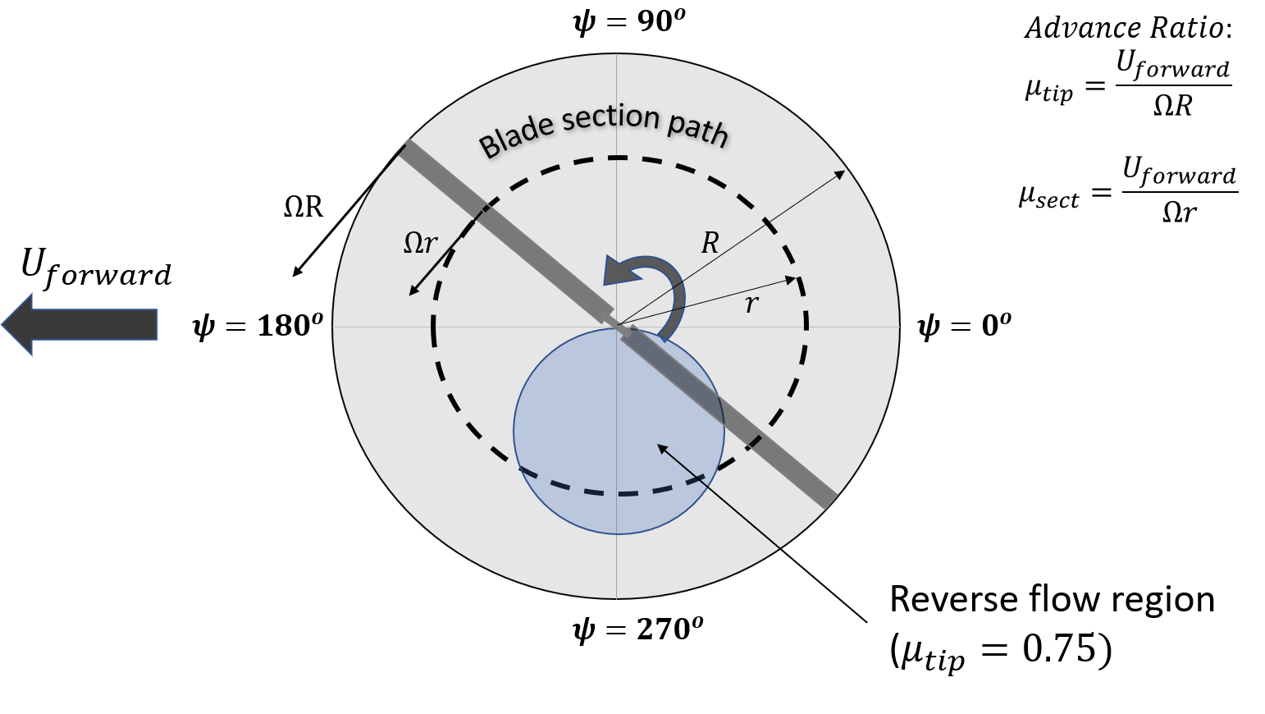
\includegraphics[width=4in]{figures/Setup/forward_flight_schematic.png}
	\caption{Top view of the rotor plane of a rotorcraft in a forward flight with reverse flow region}
	\label{fig:forward_flight_schematic}
\end{figure}

In this work, we perform LES of surging airfoils at high advance ratios.
To reduce the massive flow separation that results due to flow reversal, we employ active flow control in the form of active reflex camber, where the airfoil shape is dynamically morphed to make it more streamlined to the incoming reverse flow.

A NACA 0012 airfoil at a high Reynolds number of $Re=1,000,000$ for angle of attack of $\alpha=6^\circ$ and advance ratios of $\mu_{sect}=1.5$ and $2.0$ are considered here.
An SC1095 airfoil, which is used in the inboard region of the rotor blades for a UH-60A helicopter, is also considered here for $Re=1,000,000$ at angle of attack of $\alpha=6^\circ$ and advance ratios of $2.0$.
Active reflex camber is applied to these cases, and results are compared against the non-actuated case.
Significant reduction in flow separation in the reverse flow region is observed, along with significant reduction in drag and its fluctuations.
 

\section{Problem Setup}

In this section, we focus only on high Reynolds number flow ($Re=1,000,000$) at higher angle of attack of $\alpha=10^\circ$ and sectional advance ratios of $\mu_{sect}= 1.5$ and $2.0$. 
These advance ratios include a significant portion of the retreating phase with negative relative velocity or a reversed flow condition. 
In this reverse flow condition, massive flow separation near the geometric trailing edge is observed, and as a result, a force is experienced by the airfoil along the surging direction. 
We try to mitigate this by applying active flow control in the form of active reflex camber. 

The case with active reflex camber is referred as the actuated case.
In the actuated case, the (geometric) trailing edge is deflected up by an angle of $\beta_{TE}$=$\alpha$=10$^\circ$, with the hinge point at the 3/4th or 75\% chord location (i.e., close to the trailing edge).
The reflex camber is applied smoothly over a short period of time (both at activation and deactivation).
The full reflex/deflection is achieved just before the reverse flow regime is encountered by the airfoil in the retreating phase, and the airfoil starts to return to its original/undeflected shape once the airfoil is out of the reverse flow.

Figure \ref{fig:U_rel} shows the variation of $\tilde{U}_{rel}$ over the cycle at sectional advance ratio of $\mu_{sect}=1.5$ (blue dashed line) and $2.0$ (green solid line).
The region with $\tilde{U}_{rel}<0$ shows the phases when reverse flow is encountered by the airfoil.
The open circles on each curve represent the portion of the oscillation cycle when reflex camber is activated for that particular sectional advance ratio.


\begin{figure}[H]
\centering
\texttt{}		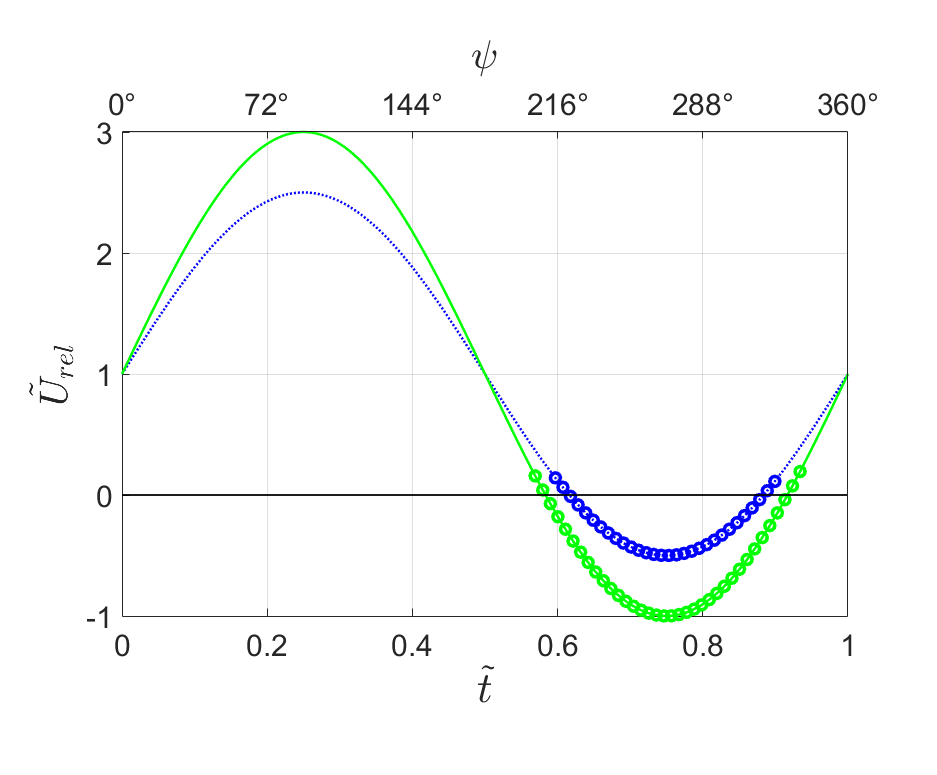
\includegraphics[width=4in]{figures/U_rel_vs_t_tilde_without_lines.png}
		\caption{Variation of $\tilde{U}_{rel}$ at $\mu_{sect}=1.5$ (green solid line) and $2.0$ (blue dashed line), open circles on each curve represent the portion of the oscillation cycle when reflex camber is activated}
		% with $\tilde{t}$ for $\lambda = 1.5$; shaded region where actuated camber is employed; red vertical lines showing instances where data is captured}
		\label{fig:U_rel}
\end{figure}

\section{Summary of Cases}

Table~\ref{table:summary_cases_AC} provides a summary of the current cases. $\beta_{TE}=0$ refers to the non-actuated case while $\beta_{TE}=\alpha$ is the actuated case.

\begin{table}[H]
	\centering
	\caption{Summary of surging cases for LES at very high advance ratios}
	\label{table:summary_cases_AC}
	\begin{tabular}{|l|c|c|c|c|c|}
		\hline
		Airfoil   & $\alpha$ & $k$ & $\mu_{sect}$ & $Re$ (mean) & $\beta_{TE}$\\
		\hline
		\hline
		NACA 0012 & 10$^\circ$ & $0.133$ & \{1.5, 2.0\} & 1,000,000 & \{0,$\alpha$\} \\
		\hline
		SC1095 & 10$^\circ$ & $0.133$ & \{2.0\} & 1,000,000 & \{0,$\alpha$\} \\
		\hline
		
	\end{tabular}
	
\end{table}

Two airfoils are considered here: NACA 0012 airfoil at $\mu_{sect}=1.5$ and $2.0$, and SC1095 airfoil at $\mu_{sect}=2.0$, both at $Re = 1,000,000$.
The computational domain and boundary conditions for this case are similar to the one mentioned in Section \ref{sec:problem_setup_baseline}.
Also, as noted earlier, an ALE description is used to account for the motion and deformation of the airfoil.
Mesh deformation is currently prescribed based on the motion and deformation of the airfoil.
The deformed mesh due to active reflex camber is shown in Figure \ref{fig:mesh3}.

The computational domain and boundary conditions for this case are similar to the one mentioned in Section \ref{sec:problem_setup_baseline}.
Also, as noted earlier, an ALE description is used to account for the motion and deformation of the airfoil.
Mesh deformation is currently prescribed based on the motion and deformation of the airfoil.
The deformed mesh due to active reflex camber is shown in Figure \ref{fig:mesh3}.


\begin{figure}[H]
	\centering
	\begin{subfigure}[b]{0.6\textwidth}
		\centering
		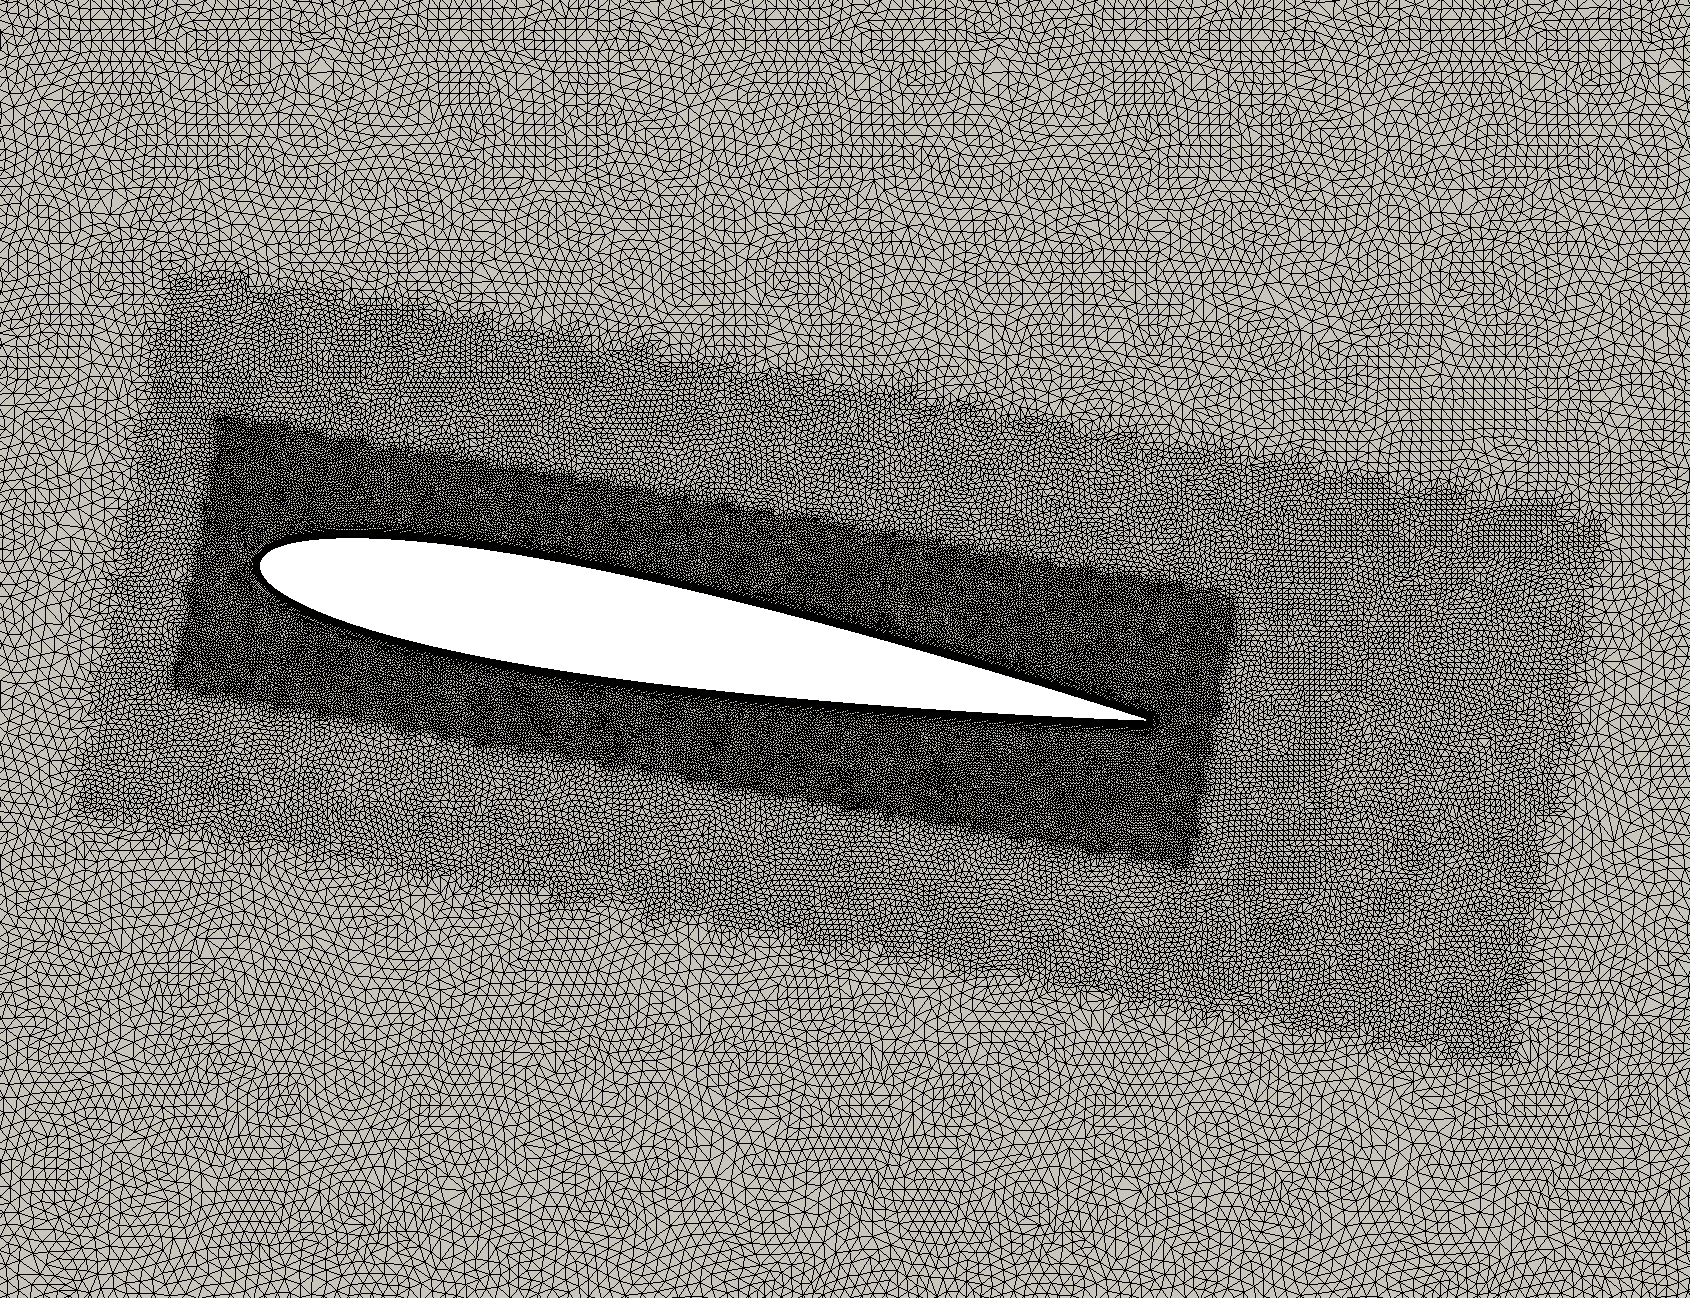
\includegraphics[width=1\textwidth]{figures/Setup/mesh}
		\caption{non-actuated case}
		\label{fig:mesh_non-actuated}
	\end{subfigure}

	\begin{subfigure}[b]{0.6\textwidth}
		\centering
		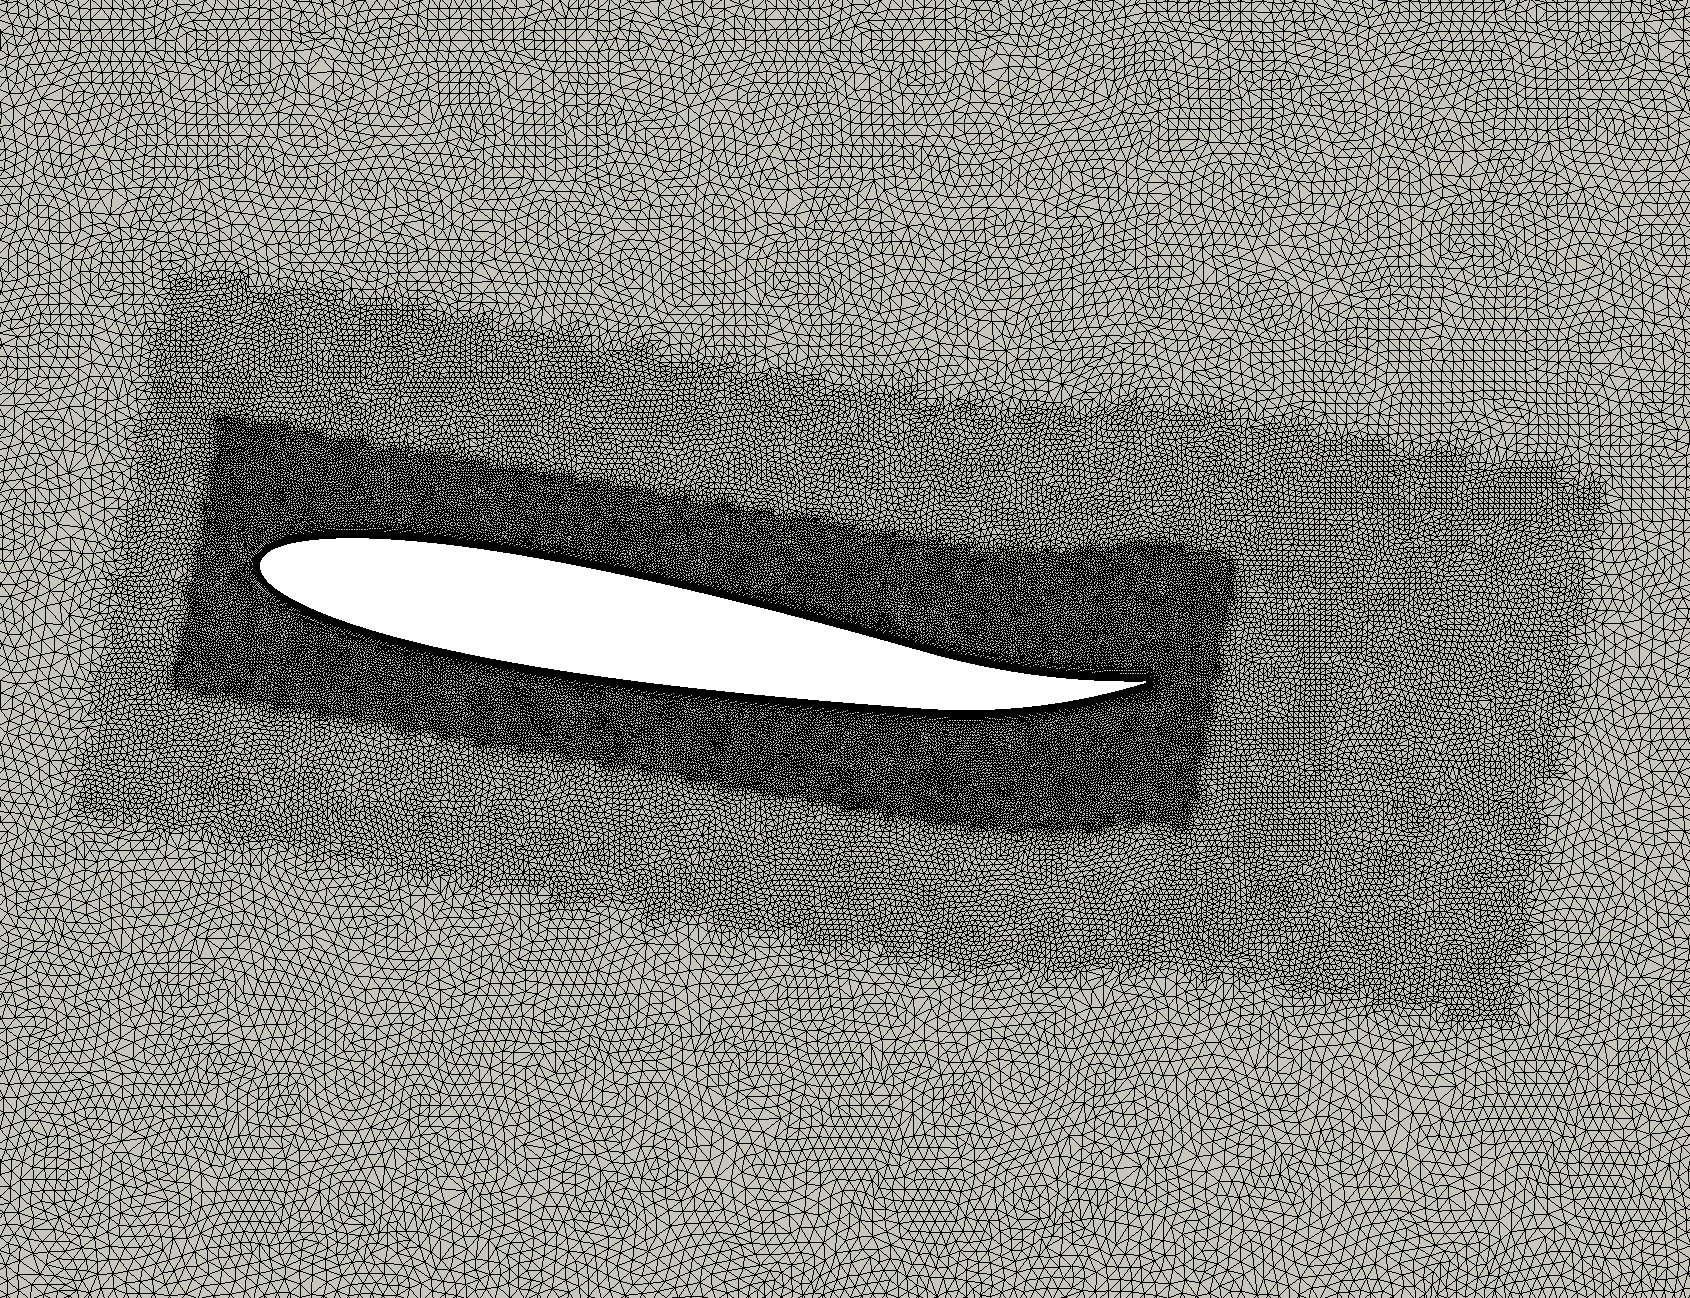
\includegraphics[width=1\textwidth]{figures/Setup/mesh_AC}
		\caption{actuated case (with reflex camber)}
		\label{fig:mesh_actuated}
	\end{subfigure}
	\caption{Mesh around the airfoil for the non-actuated and actuated cases during the reverse flow region}
	\label{fig:mesh3}
\end{figure}

\section{Results and Discussion}

\subsection{NACA 0012: $\mu_{sect} = 1.5$ and $2.0$}

\subsubsection{Force Response}

Figure \ref{fig:total_drag_zoomed_mu_1pt5} shows the behavior of the total drag in the reverse flow region for NACA 0012 airfoil for the baseline and actuated cases at $\mu_{sect}=1.5$. The total drag is normalized with the total drag of the static case ($\mu_{sect}=0.0$) at the mean Reynolds number. 
This normalization is used to be able to compare simulation and experimental data, where experiments involve tunnel effects such as walls and mounts (e.g., see \cite{bib:kocher2017}).
It also avoids the indeterminate value at the point of reverse flow when instantaneous dynamic pressure (based on the relative velocity of the airfoil) is used for normalization.

In Figure \ref{fig:total_drag_zoomed_mu_1pt5}, the drag is negative in the majority of the reverse flow region.
The negative drag value implies that it acts in the opposite direction, i.e., it acts from the geometric trailing edge towards the leading edge, which is caused due to the negative relative velocity in the reverse flow region.
In the actuated case, the negative drag value is reduced.
We note that from a rotorcraft perspective a higher negative value of the sectional drag during the retreating phase results in a higher total rotor drag (i.e., H-force).

In addition, in the baseline case the drag fluctuates around $\psi=270^\circ$ (i.e., around the peak of reverse flow), which is not the case in the actuated case.
In the baseline case, the drag exhibits a local maximum around $\psi=235^\circ$ and a local minimum around $\psi=265^\circ$.
This observation complies with that made in the flowfield (see Figure \ref{fig:vortScreen_mu1pt5}), i.e., the size of the trailing-edge separation bubble is relatively smaller and fairly constant in the actuated case.

\begin{figure}[H]
	
	\centering
	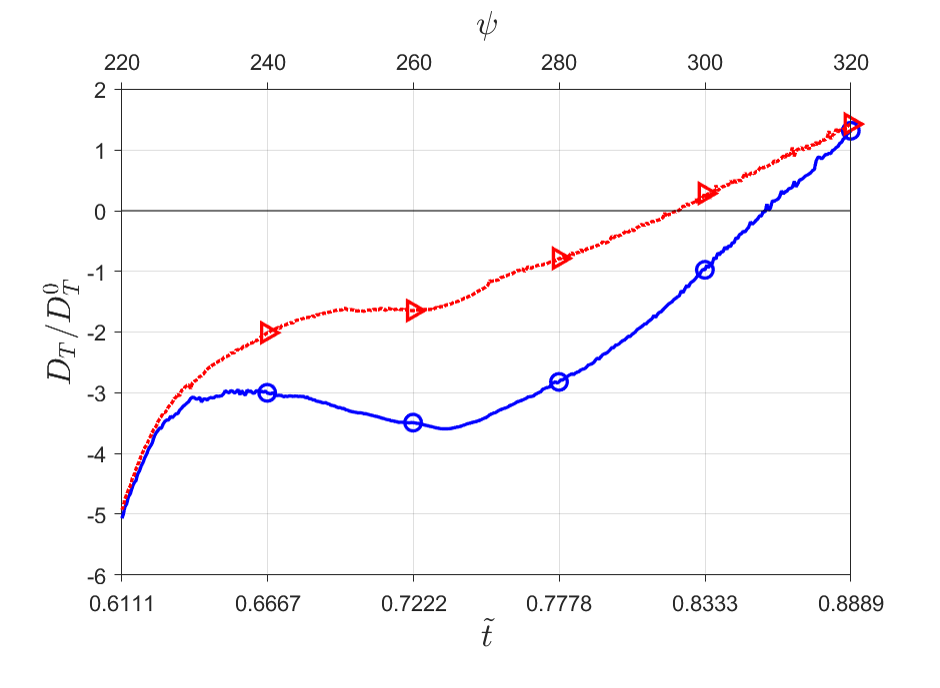
\includegraphics[width=0.75\textwidth]{figures/Zoomed_Drag_tot_NACA0012_Re1m_aoa10_1pt5_3.png}
	\caption{Normalized total drag in the reverse flow region for the baseline (blue with open circles) and actuated (red with open triangles) cases at $\mu_{sect}=1.5$}
	\label{fig:total_drag_zoomed_mu_1pt5}
\end{figure}


%	\begin{subfigure}[b]{0.45\textwidth}
	%		\centering
	%		\includegraphics[width=1\textwidth]{figures/Zoomed_Drag_tot_NACA0012_Re1m_aoa10_2.png}
	%		\caption{ $\psi$ = $195^\circ$, $\tilde{t}=0.542$}
	%		\label{fig:mu_2pt0_AC_psi195}
	%	\end{subfigure}
%
%\end{figure}




Table \ref{table:D_ratios_mu_1pt5} provides the ratios of the drag for the non-actuated and actuated cases denoted as $D^{non-act}$ and $D^{act}$, respectively.
This is done for different components of the drag, namely, total drag ($D_T$) along with pressure ($D_p$) and viscous ($D_v$) components.
Three phases of $\psi=240^\circ$, $255^\circ$ and $270^\circ$ are considered.


\begin{table}[H]
	%\begin{wraptable}[10]{l}[.005in]{3in}
	\vspace{0cm}
	\centering
	\caption{Surging cases with active camber at $\mu_{sect} = 1.5$: drag ratios}
	\label{table:D_ratios_mu_1pt5}
	\begin{tabular}{|l|c|c|c|}
		\hline
		$ \psi$   & {\large $\frac{D^{act}_{T}}{D^{non-act}_{T}}$} & {\large $\frac{D^{act}_{p}}{D^{non-act}_{p}}$} & {\large $\frac{D^{act}_{v}}{D^{non-act}_{v}}$} \\
		\hline
		\hline
		$240^\circ$ & 0.67 & 0.66 & 1.06   \\
		\hline
		$255^\circ$ & 0.48 & 0.47 & 1.16   \\
		\hline
		$270^\circ$ & 0.37 & 0.35 & 2.28   \\
		\hline
		%		$285^\circ$ & 0.23 & 0.24 & -1.11   \\
		%		\hline
	\end{tabular}
\end{table}
%\end{wraptable}

At $\psi=240^\circ$, the total drag in the actuated case is about 0.67 times of the total drag in the baseline case, i.e., about 33\% drag reduction. At $\psi=255^\circ$ and $270^\circ$, the drag ratios are 0.48 and 0.37, respectively, i.e., about 52\% and 63\% drag reduction respectively.
The pressure drag ratios are very similar to the total drag ratios.
This is because at these phases the pressure drag accounts for about 97\% to 99\% of the total drag in the non-actuated case, and about 90\% to 94\% in the actuated case.
The viscous drag ratios are higher than 1, indicating that the viscous drag is larger in the actuated case as compared to the baseline case. 




Figure \ref{fig:total_drag_zoomed_mu_2pt0} shows the behavior of the total drag in the reverse flow region for the non-actuated and actuated cases at $\mu_{sect}=2.0$. As before, the total drag is normalized with the total drag of the static case ($\mu_{sect}=0.0$) at the mean Reynolds number. 
The drag is negative in the majority of the reverse flow region.
For $\mu_{sect}=2.0$, the reduction in the negative drag due to active reflex camber is significant.

Again, in the non-actuated case the drag fluctuates in the reverse flow region.
On the other hand, the drag is fairly monotonic in the actuated case.
In the non-actuated case, the drag exhibits a local maximum around $\psi=220^\circ$ and a local minimum around $\psi=285^\circ$.
The resulting peak-to-peak variation in the non-actuated case is substantial, as shown in Figure \ref{fig:total_drag_zoomed_mu_2pt0}.
This peak-to-peak variation in the reverse flow region is mitigated in the actuated case.
This is because the trailing-edge separation bubble in the actuated case is substantially smaller and remains fairly constant in size during the reverse flow region, see Figure ~\ref{fig:vortScreen_mu2pt0}.

\begin{figure}[H]
	
	\centering
	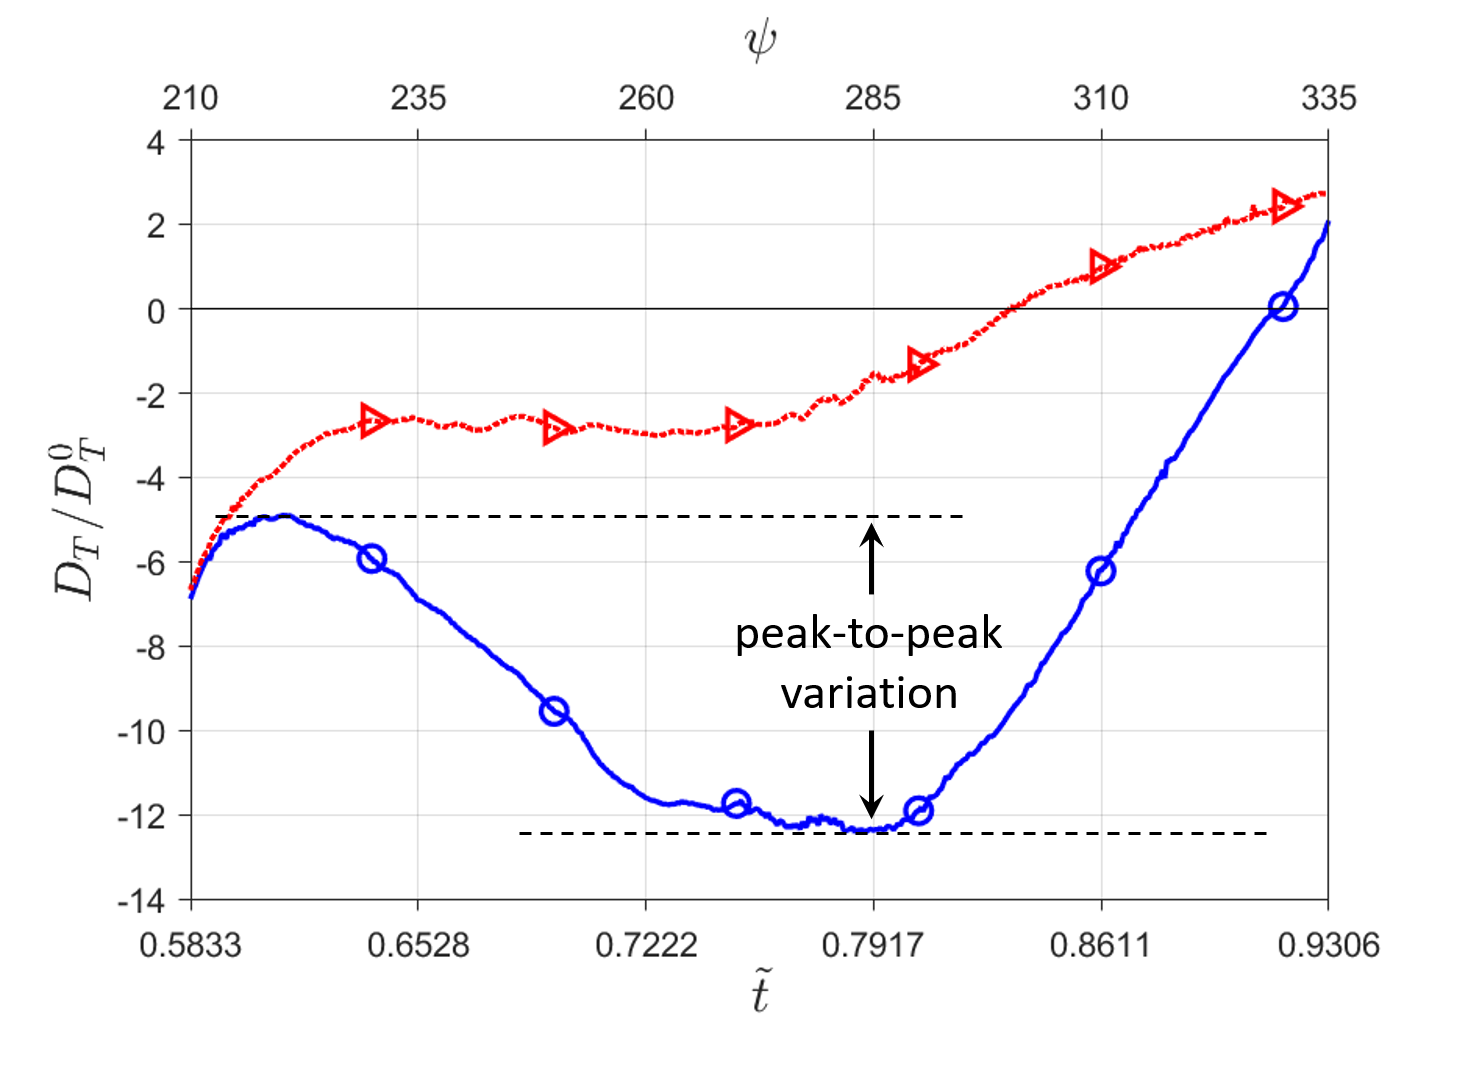
\includegraphics[width=0.75\textwidth]{figures/Zoomed_Drag_tot_NACA0012_Re1m_aoa10_3.png}
	\caption{Normalized total drag in the reverse flow region for the non-actuated (blue with open circles) and actuated (red with open triangles) cases at $\mu_{sect}=2.0$}
	\label{fig:total_drag_zoomed_mu_2pt0}
\end{figure}

Table \ref{table:D_ratios_mu_2pt0} provides the ratios of the different components of the drag at three phases. At $\psi=240^\circ$, the total drag in the actuated case is about 0.36 times of the total drag in the non-actuated case. At $\psi=255^\circ$ and $270^\circ$, the drag ratios are 0.26 and 0.24, respectively. That is we observe a reduction by up to 76\% in the total drag.
Note that the pressure drag ratios are very similar to the total drag ratios (since at these phases the pressure drag dominates over the viscous drag).

\begin{table}[H]
	%   \begin{wraptable}[10]{l}[.005in]{3in}
		\vspace{0cm}
		\centering
		\caption{Surging cases with active camber at $\mu_{sect} = 2.0$: drag ratios}
		\label{table:D_ratios_mu_2pt0}
		\begin{tabular}{|l|c|c|c|}
			\hline
			$ \psi$   & {\large $\frac{D^{act}_{T}}{D^{non-act}_{T}}$} & {\large $\frac{D^{act}_{p}}{D^{non-act}_{p}}$} & {\large $\frac{D^{act}_{v}}{D^{non-act}_{v}}$} \\
			\hline
			\hline
			$240^\circ$ & 0.36 & 0.35 & 1.44   \\
			\hline
			$255^\circ$ & 0.26 & 0.24 & 2.34   \\
			\hline
			$270^\circ$ & 0.24 & 0.22 & 4.19   \\
			\hline
			%	$285^\circ$ & 0.14 & 0.12 & -5.95   \\
			%	\hline
		\end{tabular}
	\end{table}

\subsubsection{Flowfield: Spanwise Vorticity and Velocity Magnitude}
Figure \ref{fig:vortScreen_mu1pt5} shows the instantaneous spanwise vorticity for the sectional advance ratio of $\mu_{sect}$=1.5.
8 different phases over the retreating phase of the oscillation cycle are shown. The vorticity range is selected to be [-30,30]$ U_{sect}/C$. For this sectional advance ratio, the airfoil enters the reverse flow region around $\psi=222^\circ$ and exits the reverse flow region at about $\psi$=$318^\circ$. In the actuated case, reflex camber is activated at $\psi$=$215^\circ$, and smoothly reaches the full deflection at $\psi$=$220^\circ$. After the airfoil exits the reverse flow, the reflexed airfoil starts returning to its undeflected position at $\psi$=$320^\circ$, and smoothly reaches its original shape at $\psi$=$325^\circ$.


At $\psi$=$195^\circ$, the flow over the airfoil is very similar between the baseline and actuated cases.
At $\psi$=$225^\circ$ for the actuated case, reflex camber is fully activated as seen in Figure \ref{fig:mu_1pt5_AC_psi225}. As the trailing edge is deflected upwards, a small vortex is formed just below it. Also, a roll up of the boundary layer is observed near the geometric leading edge for both baseline and actuated cases, and the formation of the leading edge vortex (LEV) begins. A more detailed analysis of the LEV at different Reynolds numbers and advance ratios was reported in \ref{sec:baseline_results}.

At $\psi$=$240^\circ$, flow separation forms near the bottom of the trailing edge of the airfoil for both baseline and actuated cases.
In the subsequent phases of the baseline case, the extent of this separated region increases along the airfoil and in the transverse direction, i.e., the separation bubble grows, till up to $\psi$=$285^\circ$. 
On the contrary, the extent of the separated region remains relatively small in the actuated case. For example, see Figures \ref{fig:mu_1pt5_baseline_psi285} and \ref{fig:mu_1pt5_AC_psi285}.
Moreover, in the actuated case the size of the separated region remains fairly constant between phases $\psi$=$255^\circ$ and $285^\circ$, see Figures \ref{fig:mu_1pt5_AC_psi255}, \ref{fig:mu_1pt5_AC_psi270} and \ref{fig:mu_1pt5_AC_psi285}.
Overall a significant reduction is observed in the size/extent as well as unsteadiness of the separation bubble near the trailing edge during the reverse flow region due to active reflex camber.
The implications of this trailing-edge separated region on the drag force is discussed in Section \ref{sec:LEV}

After $\psi$=$285^\circ$, the trailing-edge flow separation begins to wash away from the airfoil for both baseline and actuated cases.
For the actuated case at $\psi$=$330^\circ$, the reflexed trailing edge is at its undeflected position.
As the trailing edge is deflected down to its original position, this results in the formation of another small vortex as seen in Figure \ref{fig:mu_1pt5_AC_psi330}, similar to when the trailing edge is deflected up (e.g., at $\psi$=$225^\circ$ in Figure \ref{fig:mu_1pt5_AC_psi225}).

\begin{figure}[H]
	\centering
	
	\begin{subfigure}[b]{0.4\textwidth}
		\centering
		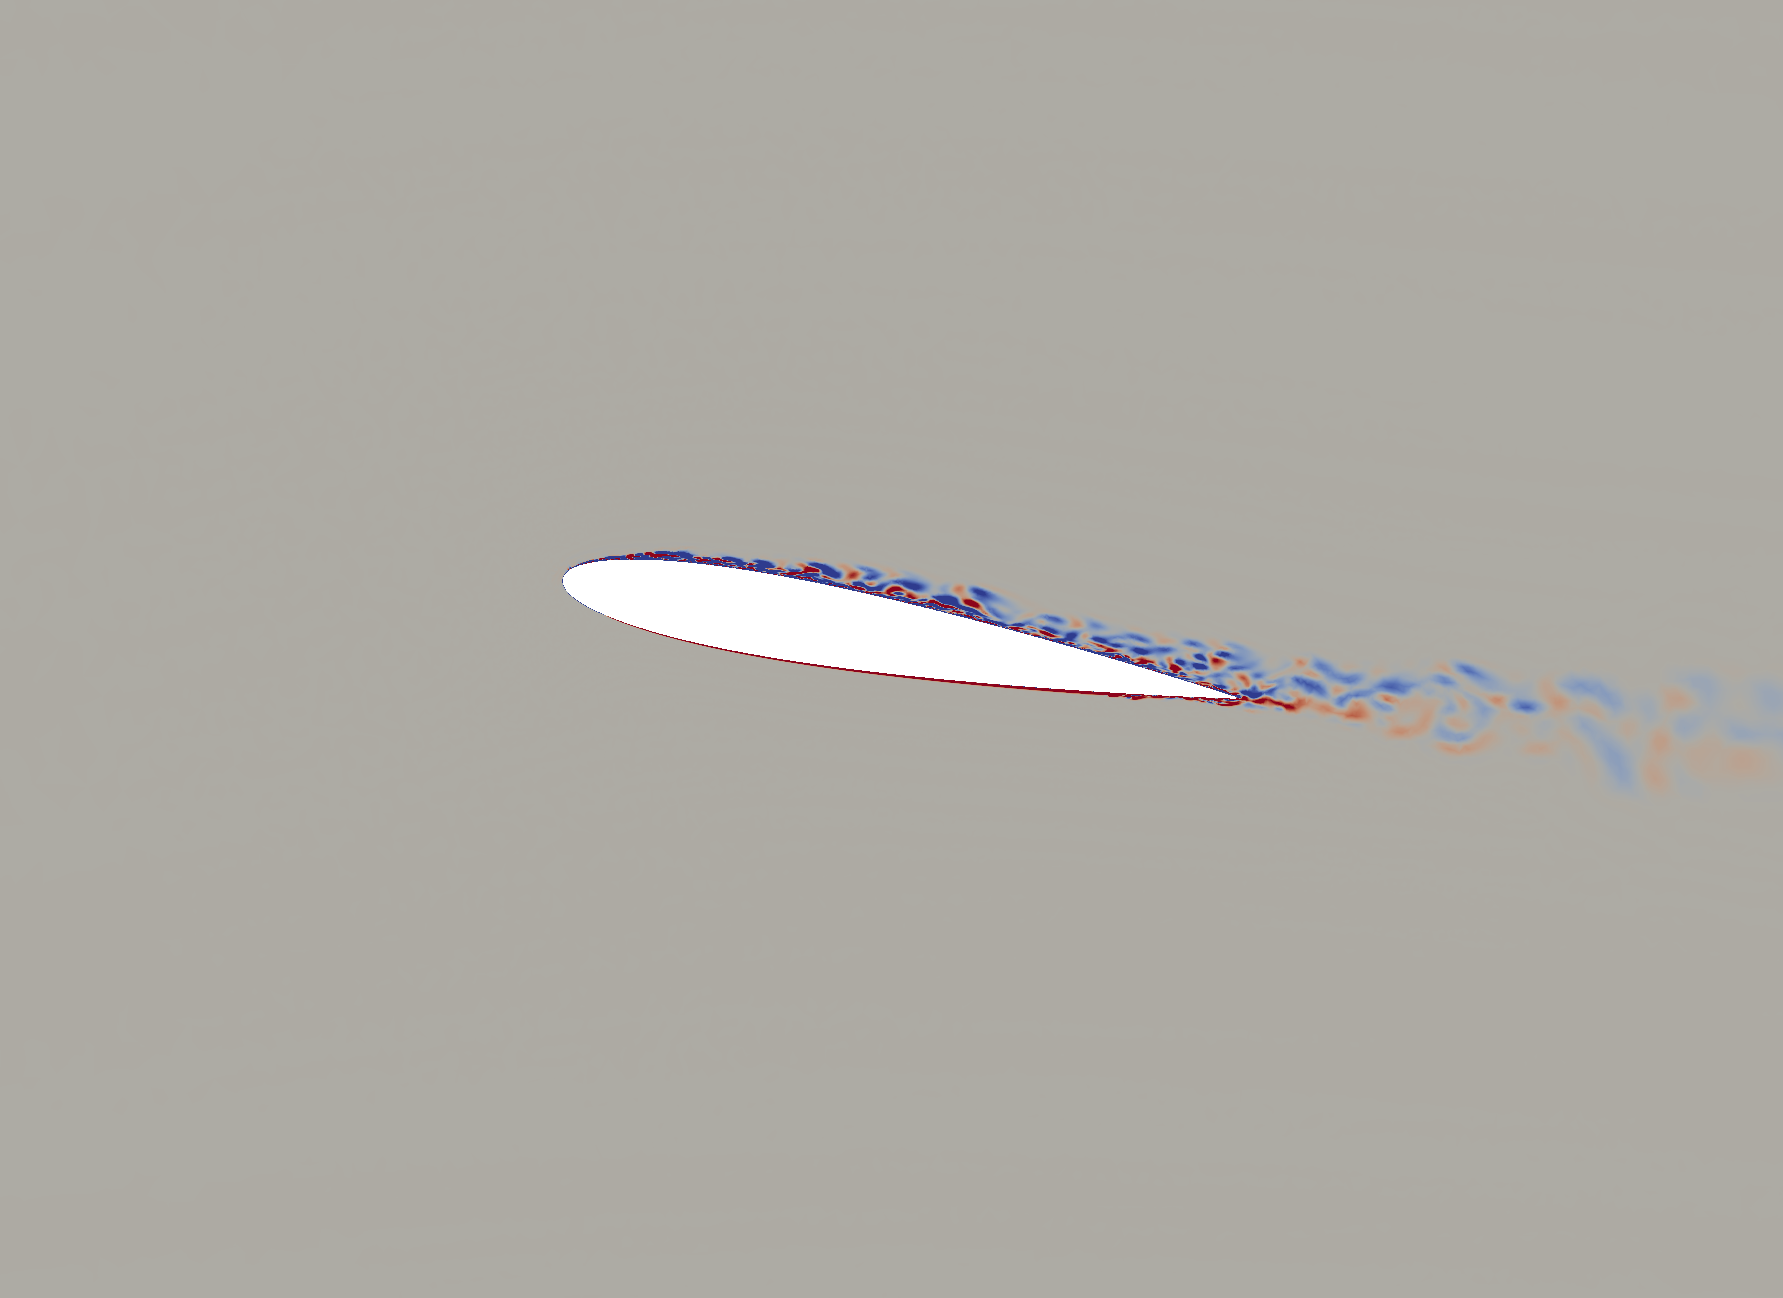
\includegraphics[width=1\textwidth]{figures/mu_1pt5/vorticity/baseline/phase_195.png}
		\caption{ $\psi$ = $195^\circ$, $\tilde{t}=0.542$}
		\label{fig:mu_1pt5_baseline_psi195}
	\end{subfigure}
	\begin{subfigure}[b]{0.4\textwidth}
		\centering
		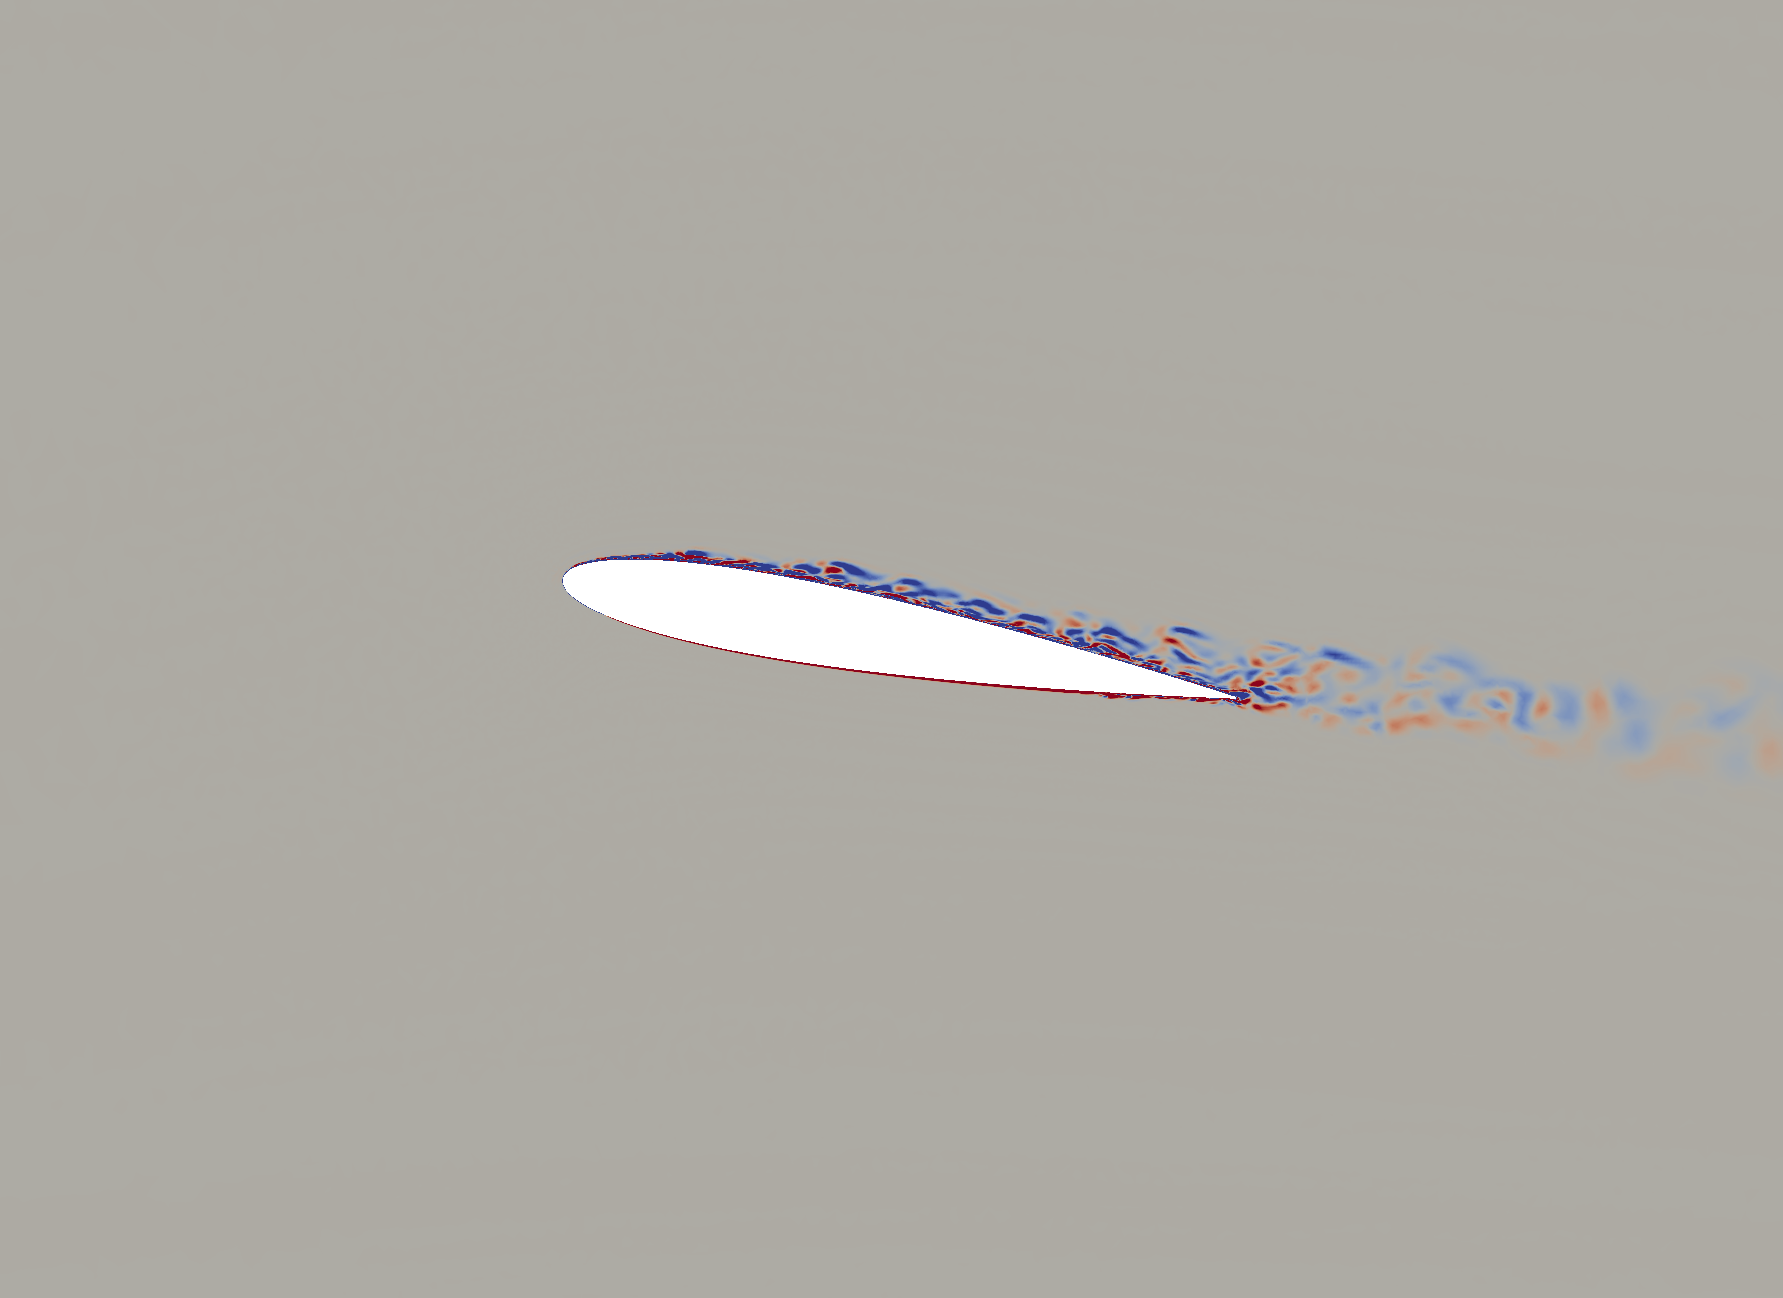
\includegraphics[width=1\textwidth]{figures/mu_1pt5/vorticity/AC/phase_195.png}
		\caption{ $\psi$ = $195^\circ$, $\tilde{t}=0.542$}
		\label{fig:mu_1pt5_AC_psi195}
	\end{subfigure}
	
	%\begin{subfigure}[b]{0.4\textwidth}
	%	\centering
	%	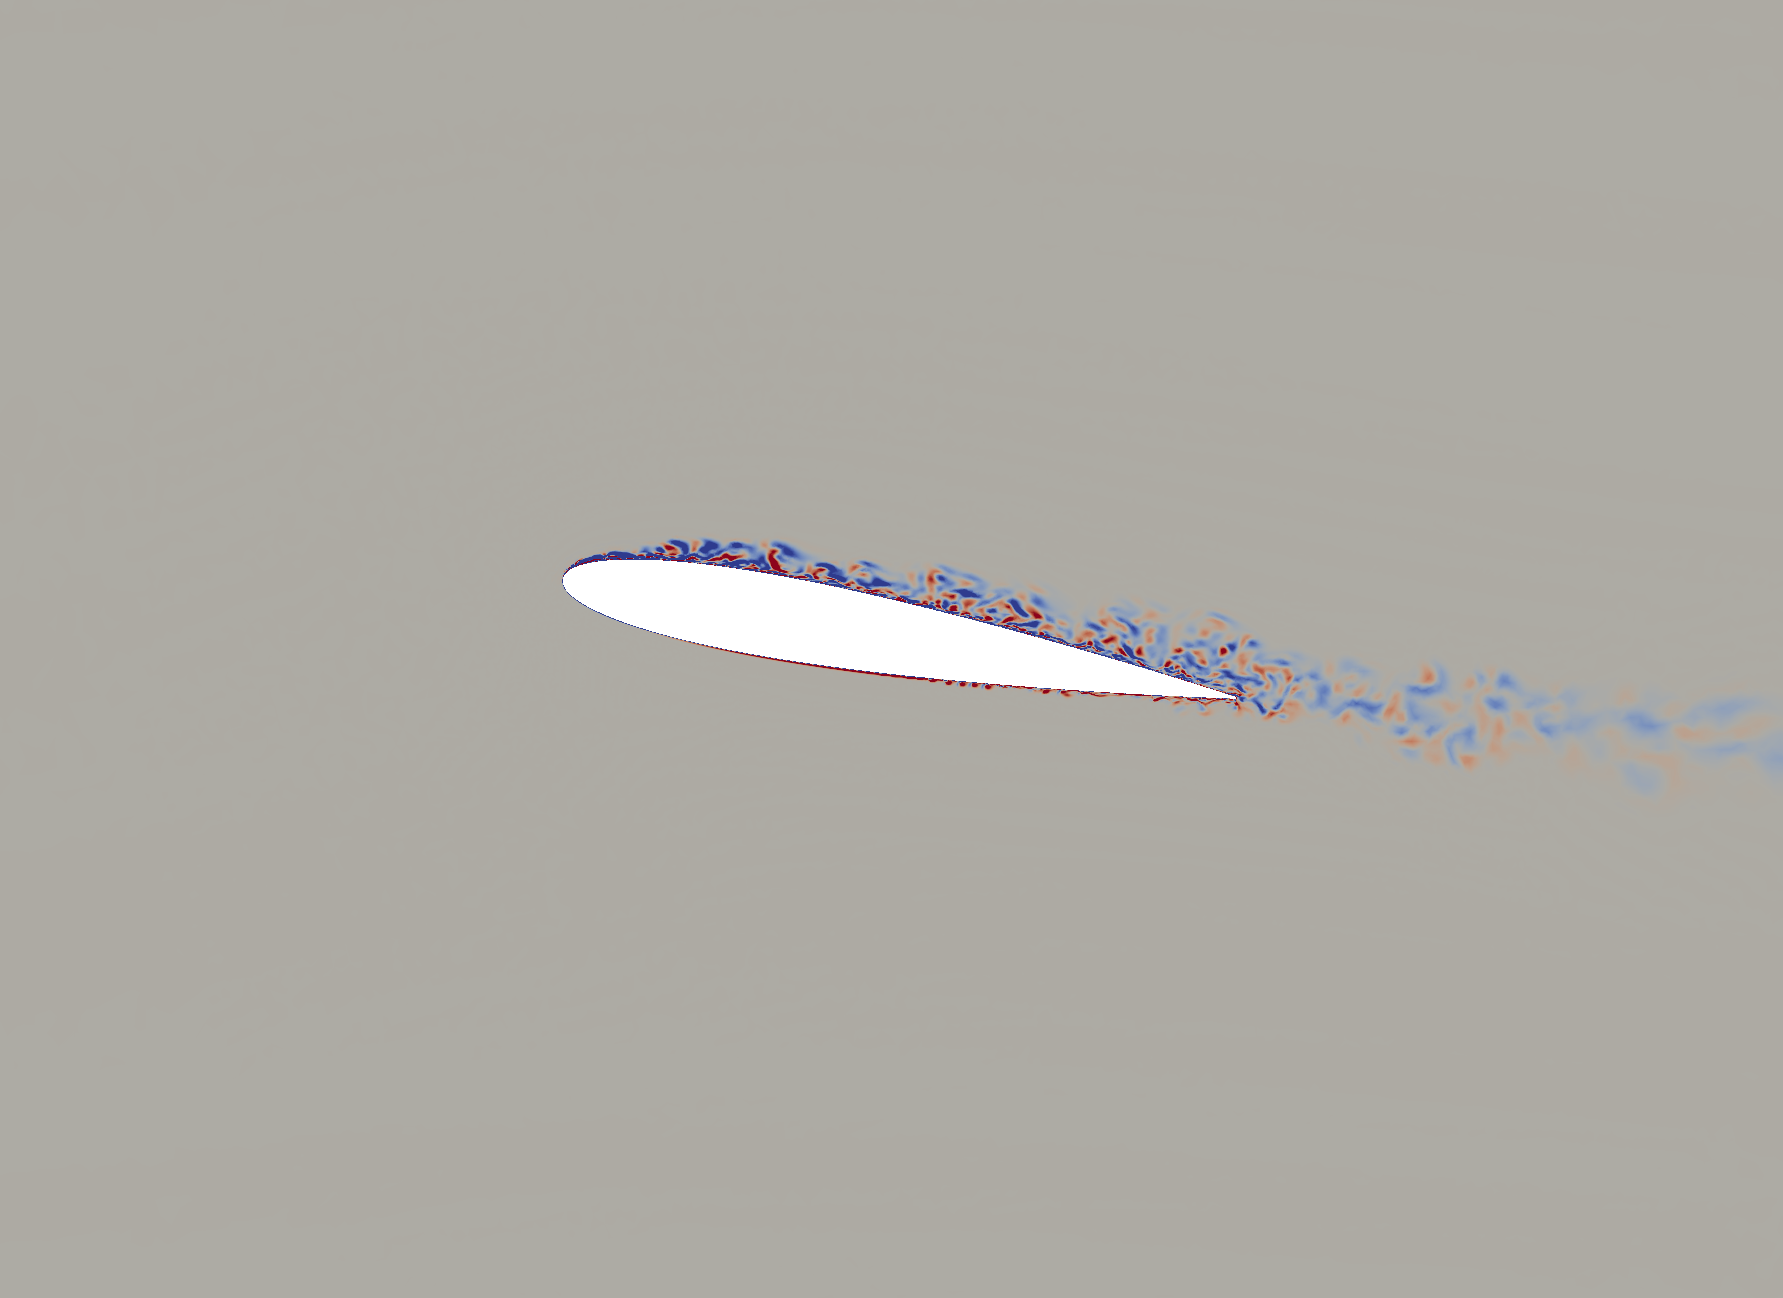
\includegraphics[width=1\textwidth]{figures/mu_1pt5/vorticity/baseline/phase_210.png}
	%	\caption{ $\psi$ = $210^\circ$, $\tilde{t}=0.583$}
	%	\label{fig:mu_1pt5_baseline_psi210}
	%\end{subfigure}
	%\begin{subfigure}[b]{0.4\textwidth}
	%	\centering
	%	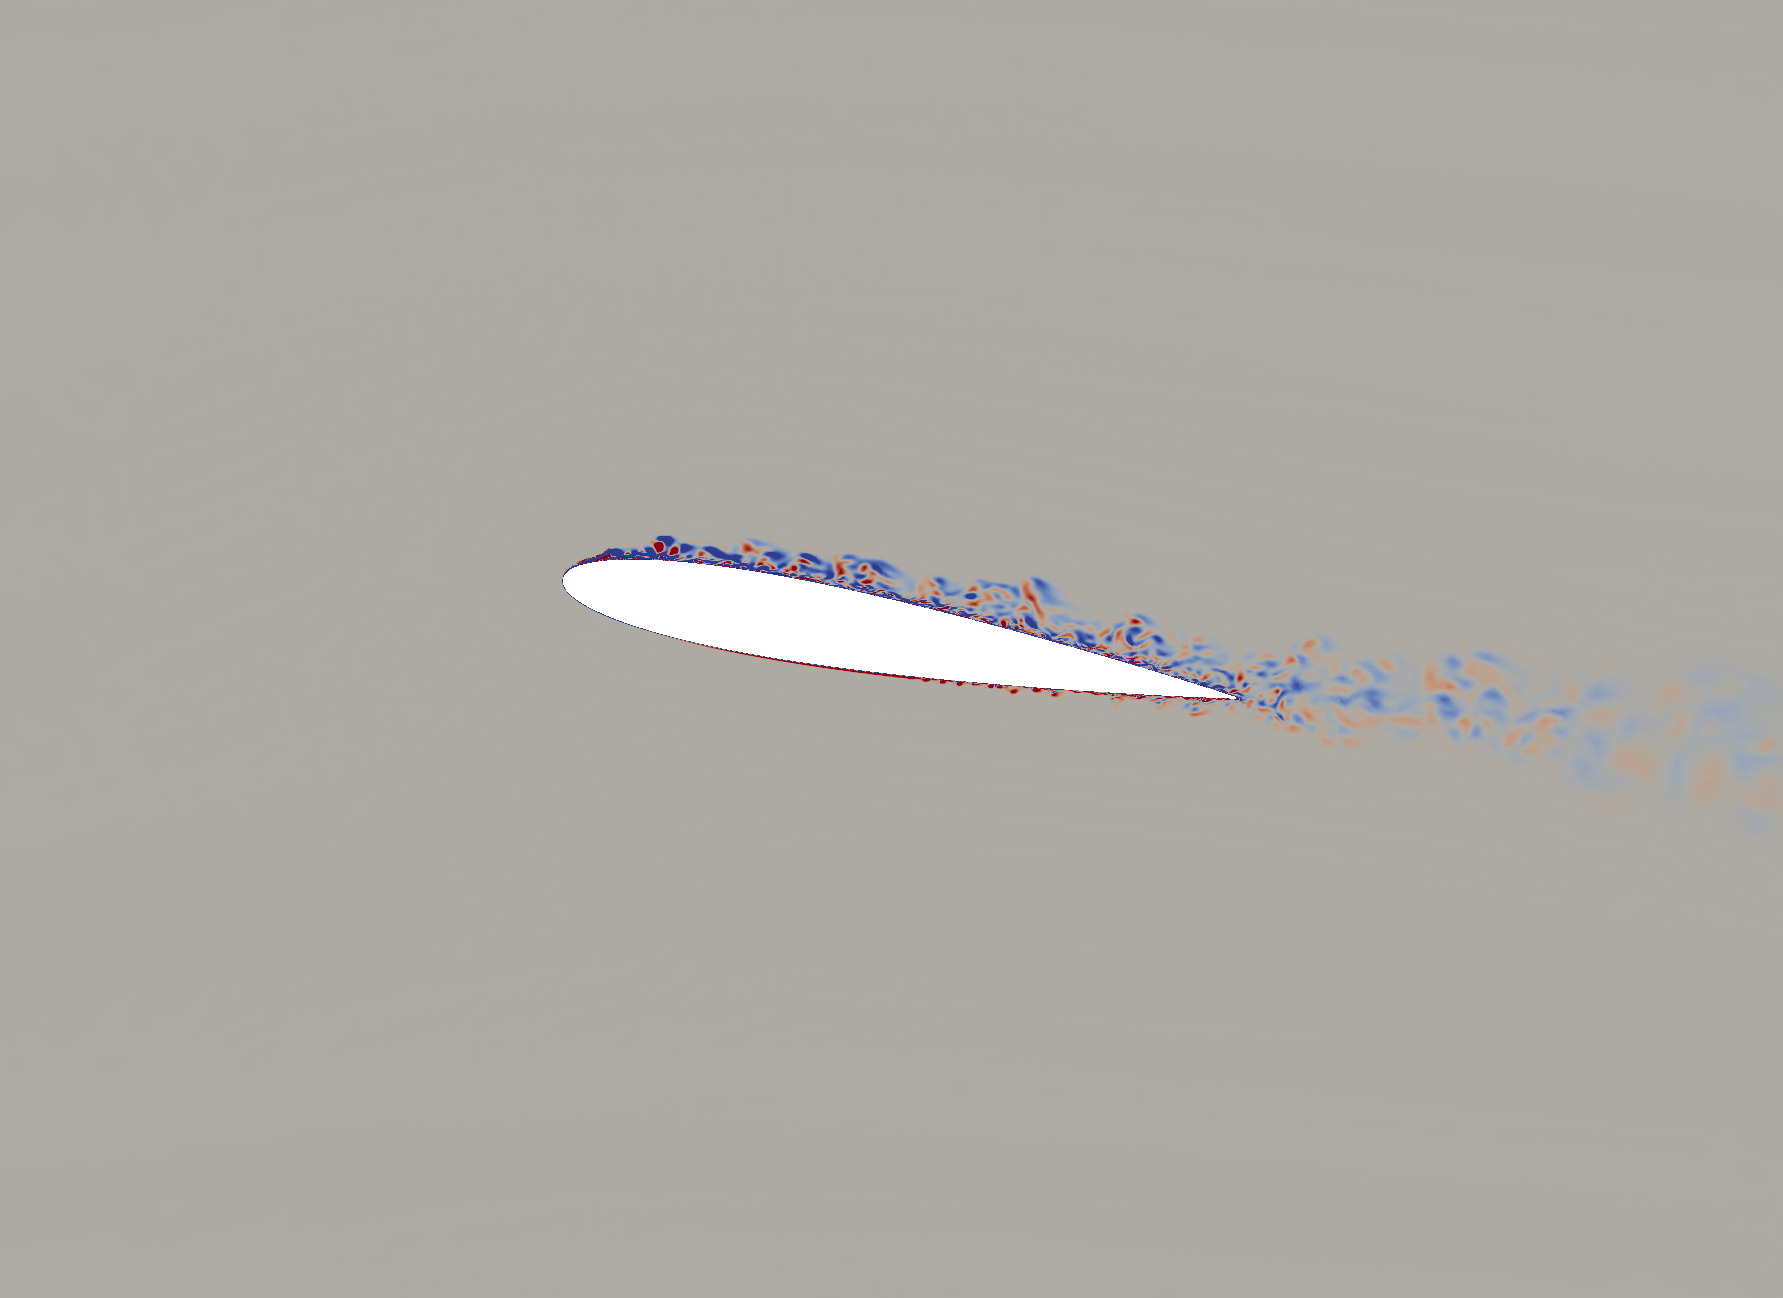
\includegraphics[width=1\textwidth]{figures/mu_1pt5/vorticity/AC/phase_210.png}
	%	\caption{ $\psi$ = $210^\circ$, $\tilde{t}=0.583$}
	%	\label{fig:mu_1pt5_AC_psi210}
	%\end{subfigure}
	
	\begin{subfigure}[b]{0.4\textwidth}
		\centering
		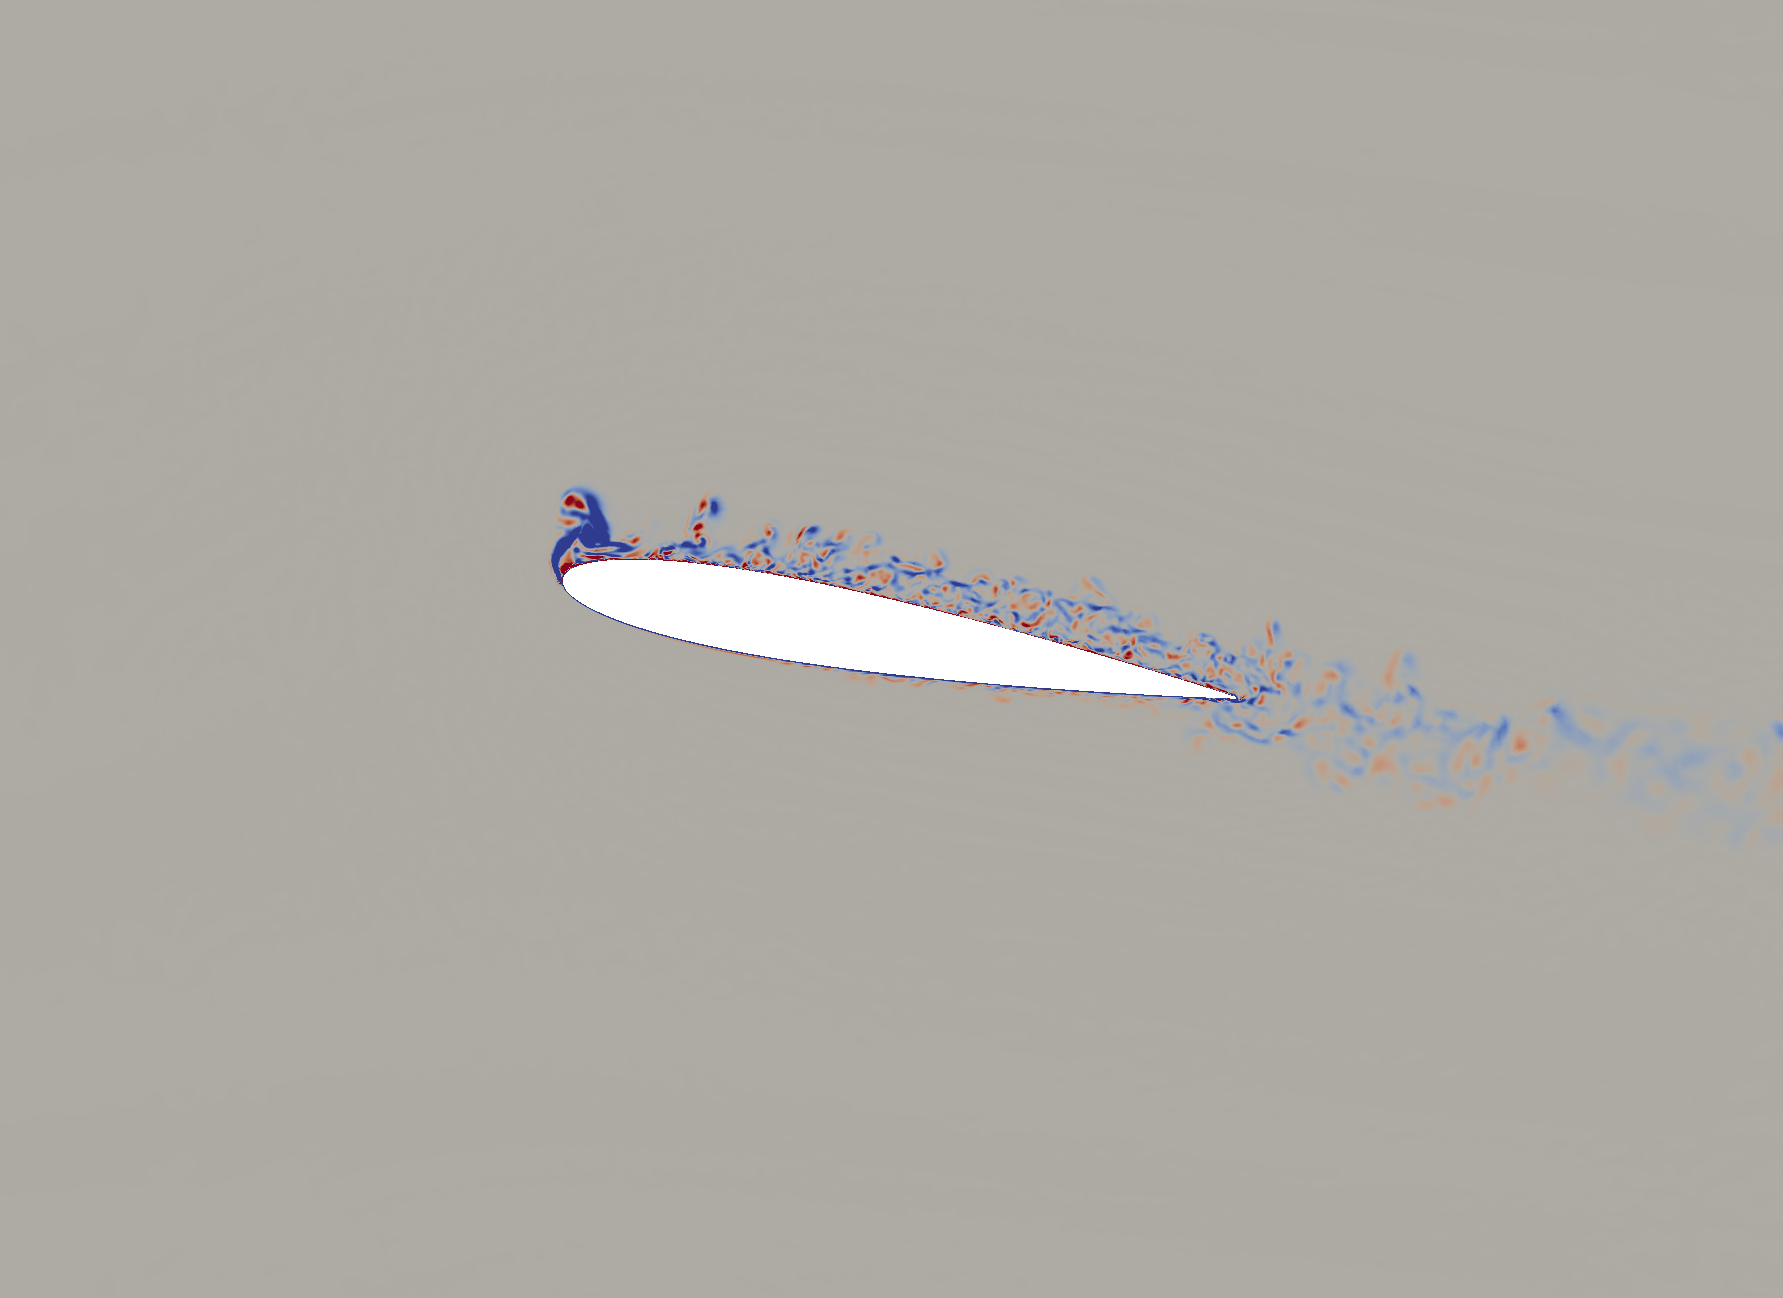
\includegraphics[width=1\textwidth]{figures/mu_1pt5/vorticity/baseline/phase_225.png}
		\caption{ $\psi$ = $225^\circ$, $\tilde{t}=0.625$}
		\label{fig:mu_1pt5_baseline_psi225}
	\end{subfigure}
	\begin{subfigure}[b]{0.4\textwidth}
		\centering
		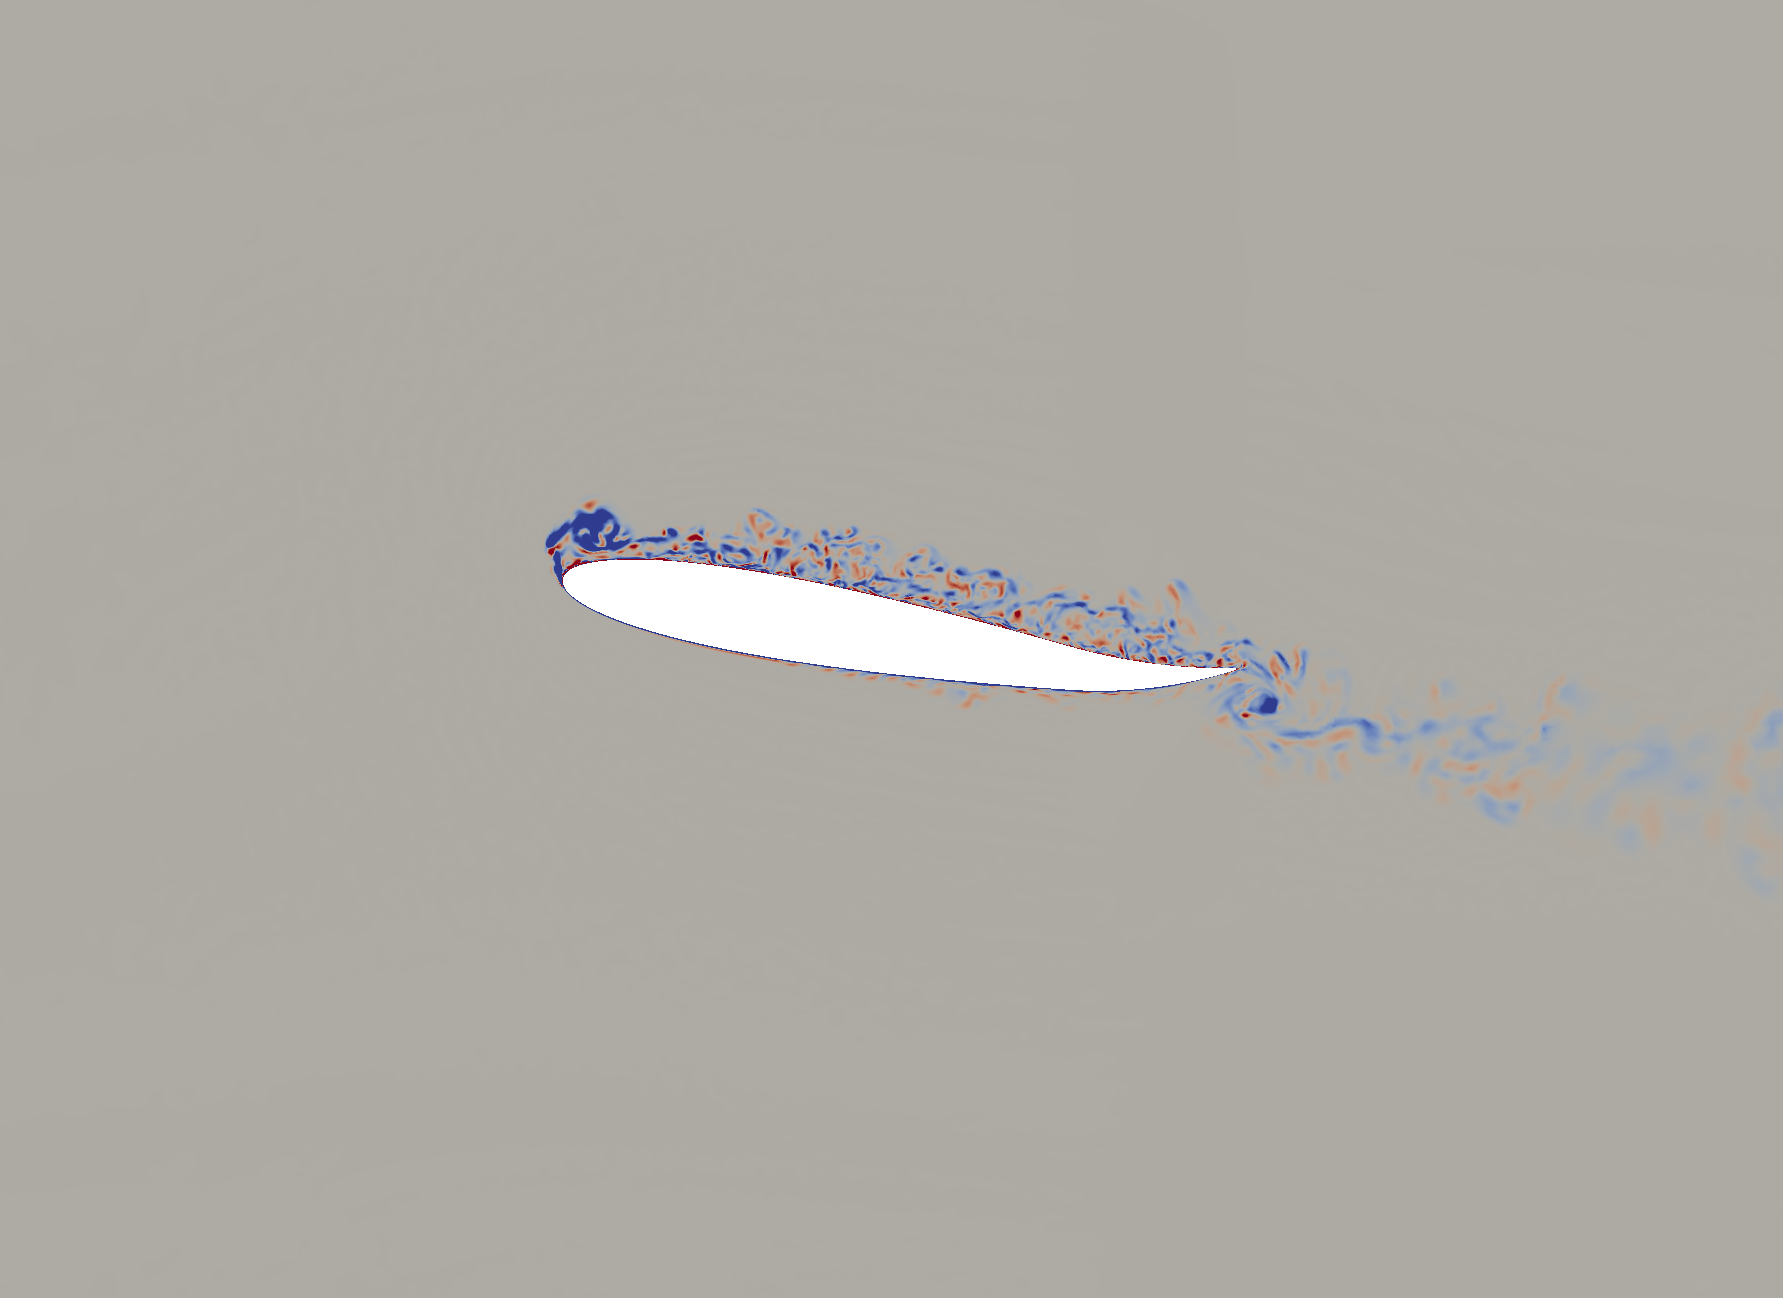
\includegraphics[width=1\textwidth]{figures/mu_1pt5/vorticity/AC/phase_225.png}
		\caption{ $\psi$ = $225^\circ$,  $\tilde{t}=0.625$}
		\label{fig:mu_1pt5_AC_psi225}
	\end{subfigure}
	
	
	\begin{subfigure}[b]{0.4\textwidth}
		\centering
		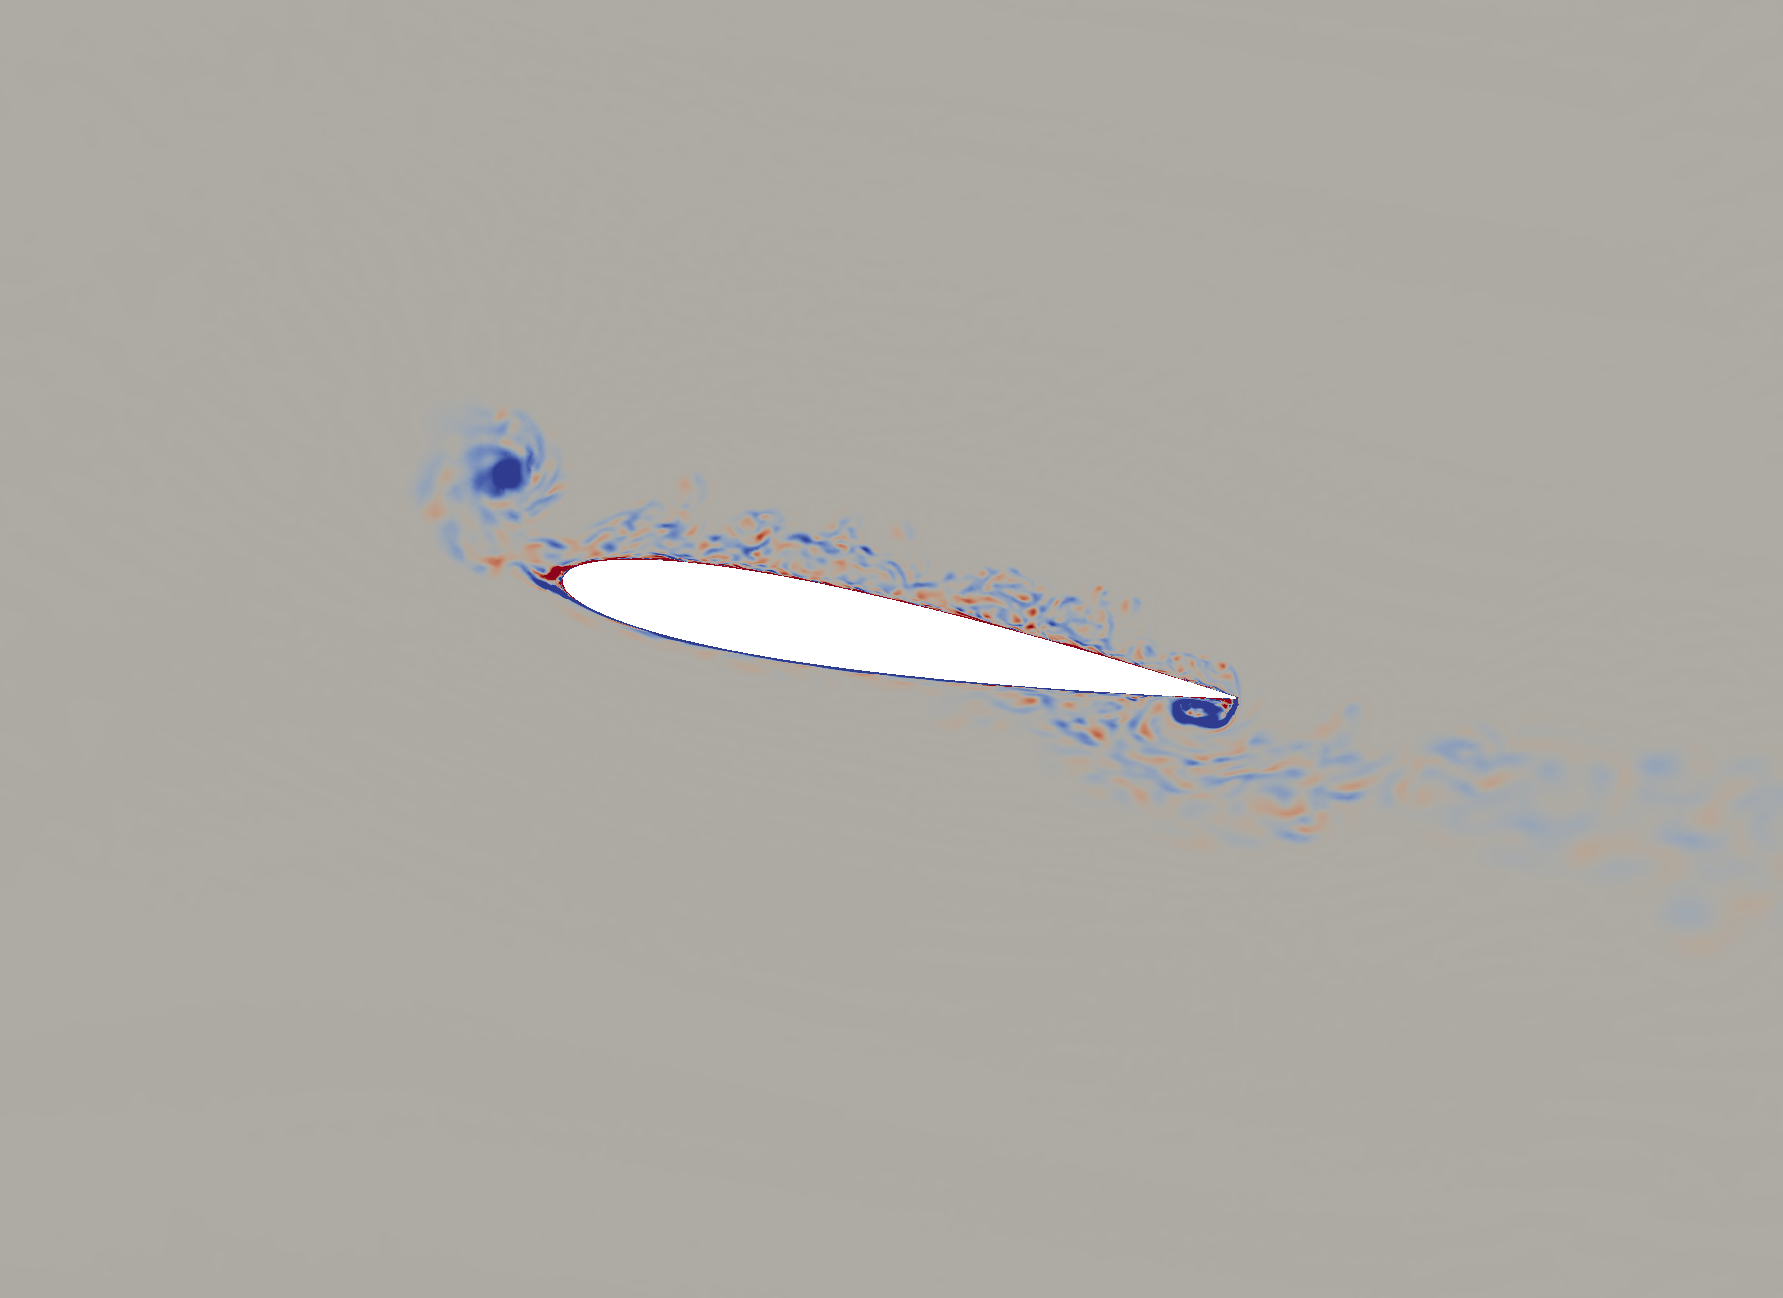
\includegraphics[width=1\textwidth]{figures/mu_1pt5/vorticity/baseline/phase_240.png}
		\caption{ $\psi$ = $240^\circ$, $\tilde{t}=0.667$}
		\label{fig:mu_1pt5_baseline_psi240}
	\end{subfigure}
	\begin{subfigure}[b]{0.4\textwidth}
		\centering
		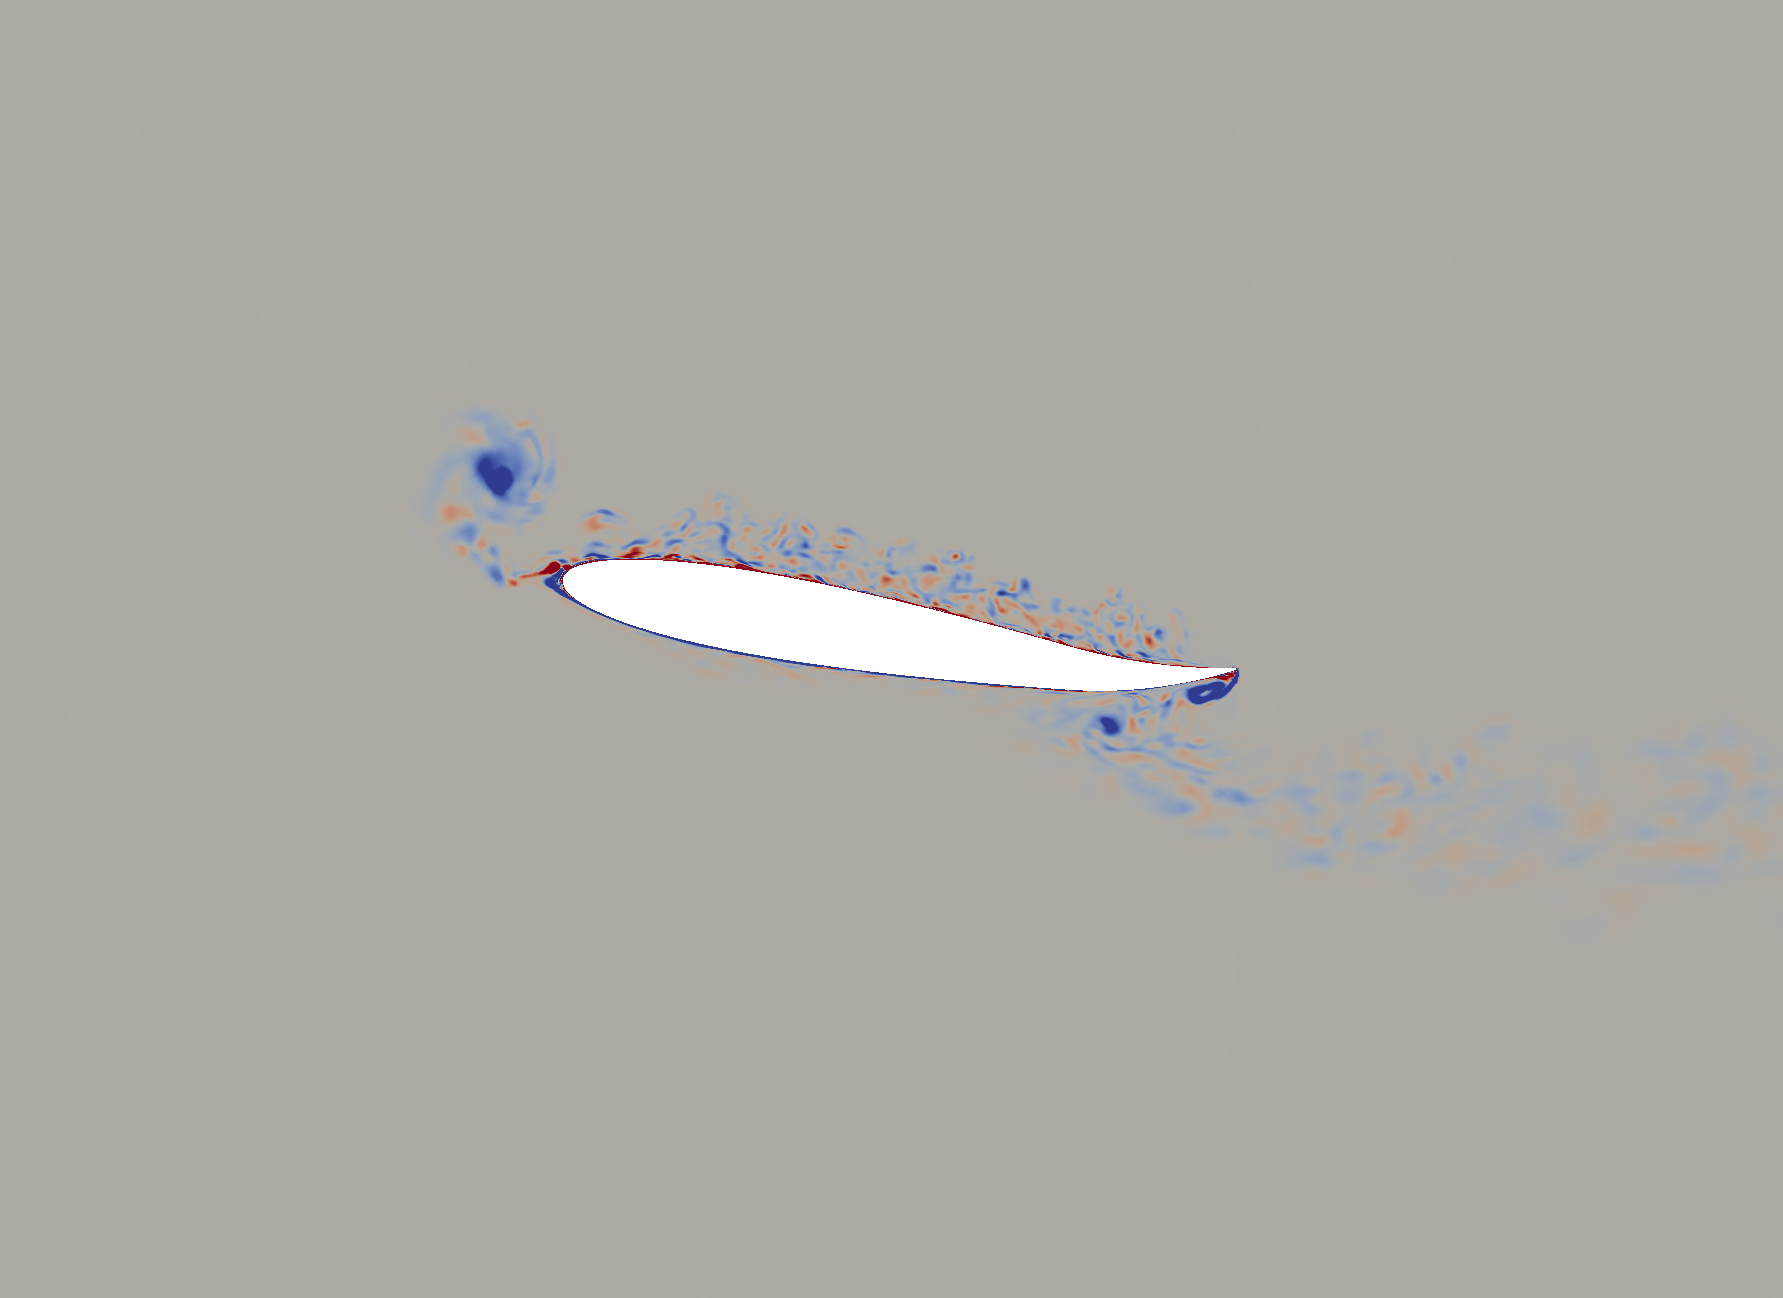
\includegraphics[width=1\textwidth]{figures/mu_1pt5/vorticity/AC/phase_240.png}
		\caption{ $\psi$ = $240^\circ$, $\tilde{t}=0.667$}
		\label{fig:mu_1pt5_AC_psi240}
	\end{subfigure}
	
	\begin{subfigure}[b]{0.4\textwidth}
		\centering
		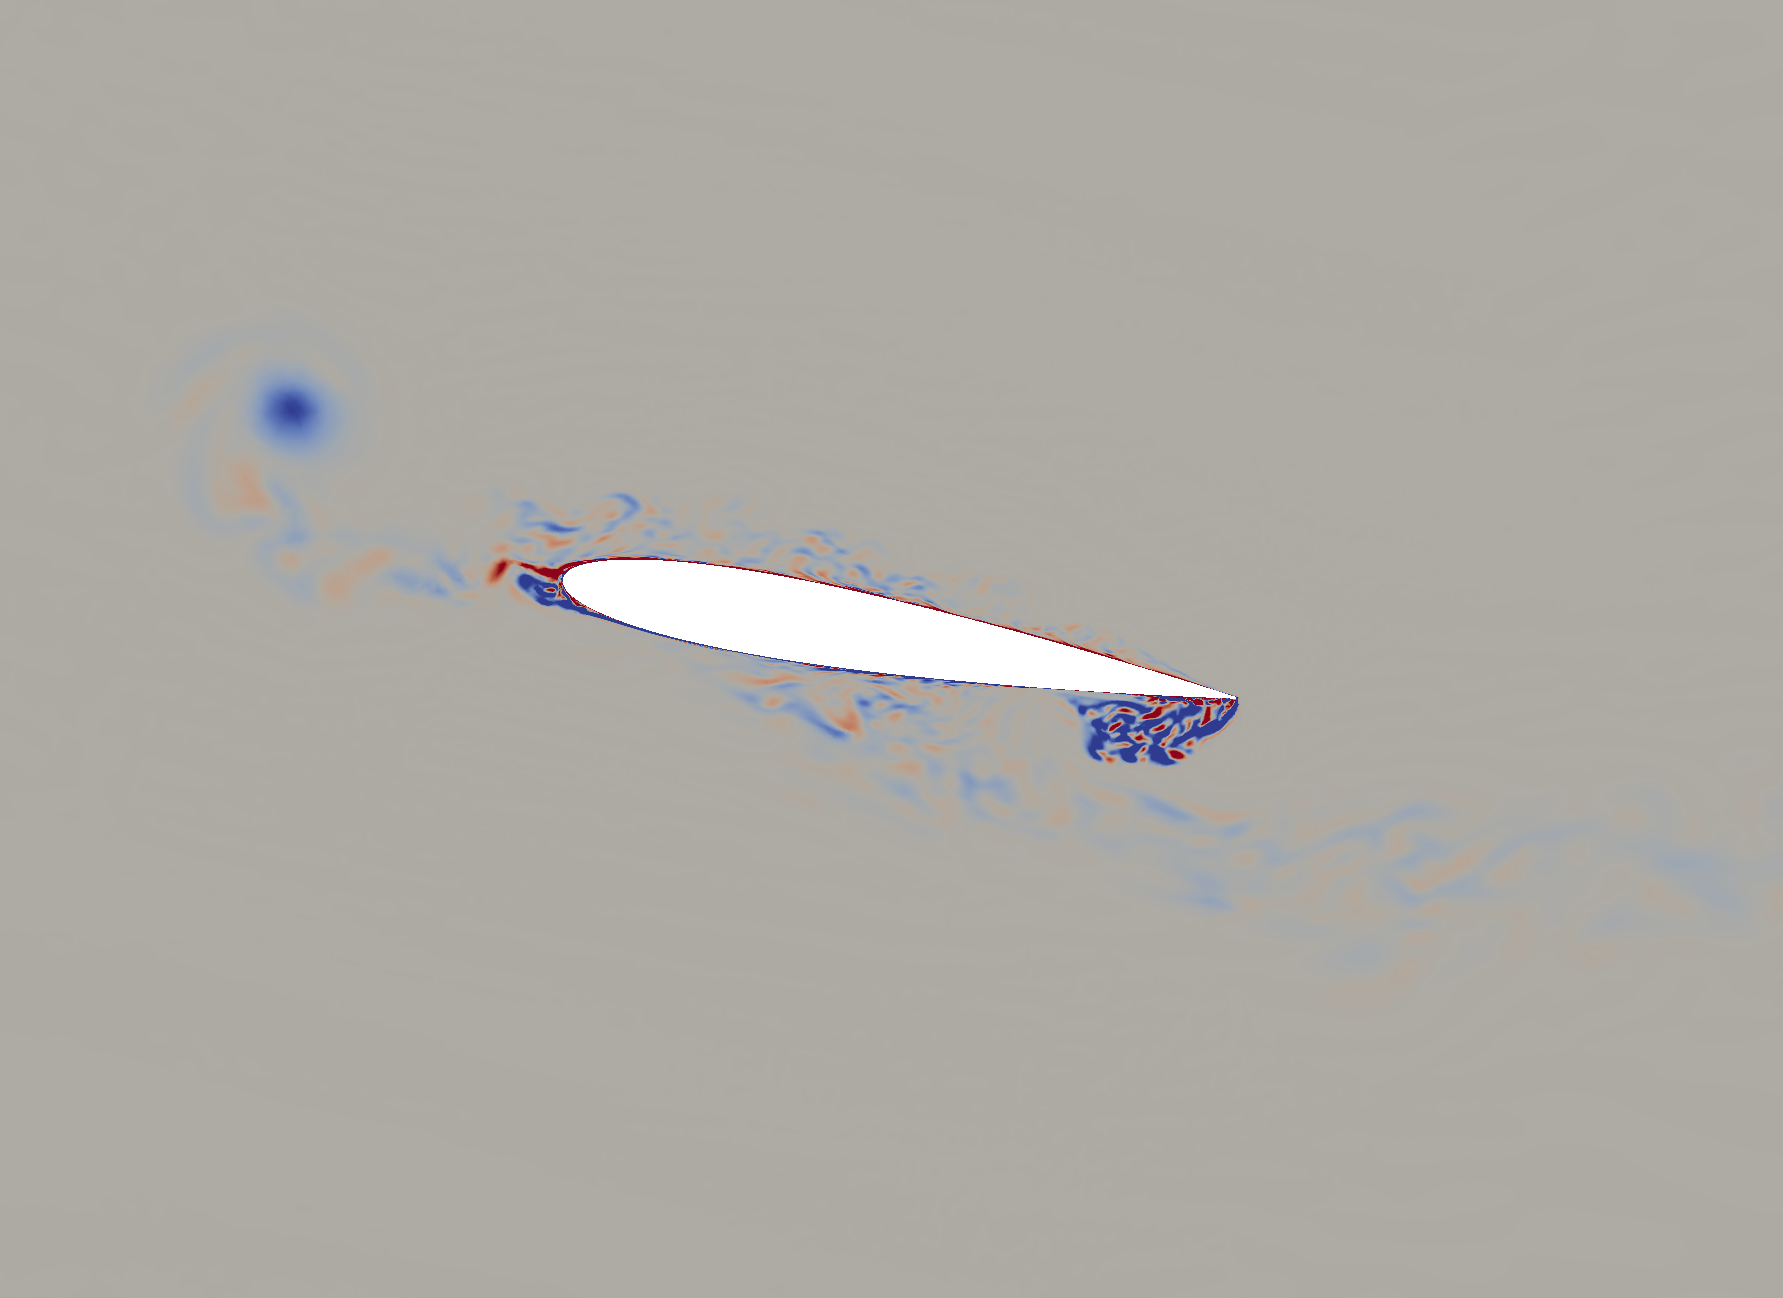
\includegraphics[width=1\textwidth]{figures/mu_1pt5/vorticity/baseline/phase_255.png}
		\caption{ $\psi$ = $255^\circ$, $\tilde{t}=0.708$}
		\label{fig:mu_1pt5_baseline_psi255}
	\end{subfigure}
	\begin{subfigure}[b]{0.4\textwidth}
		\centering
		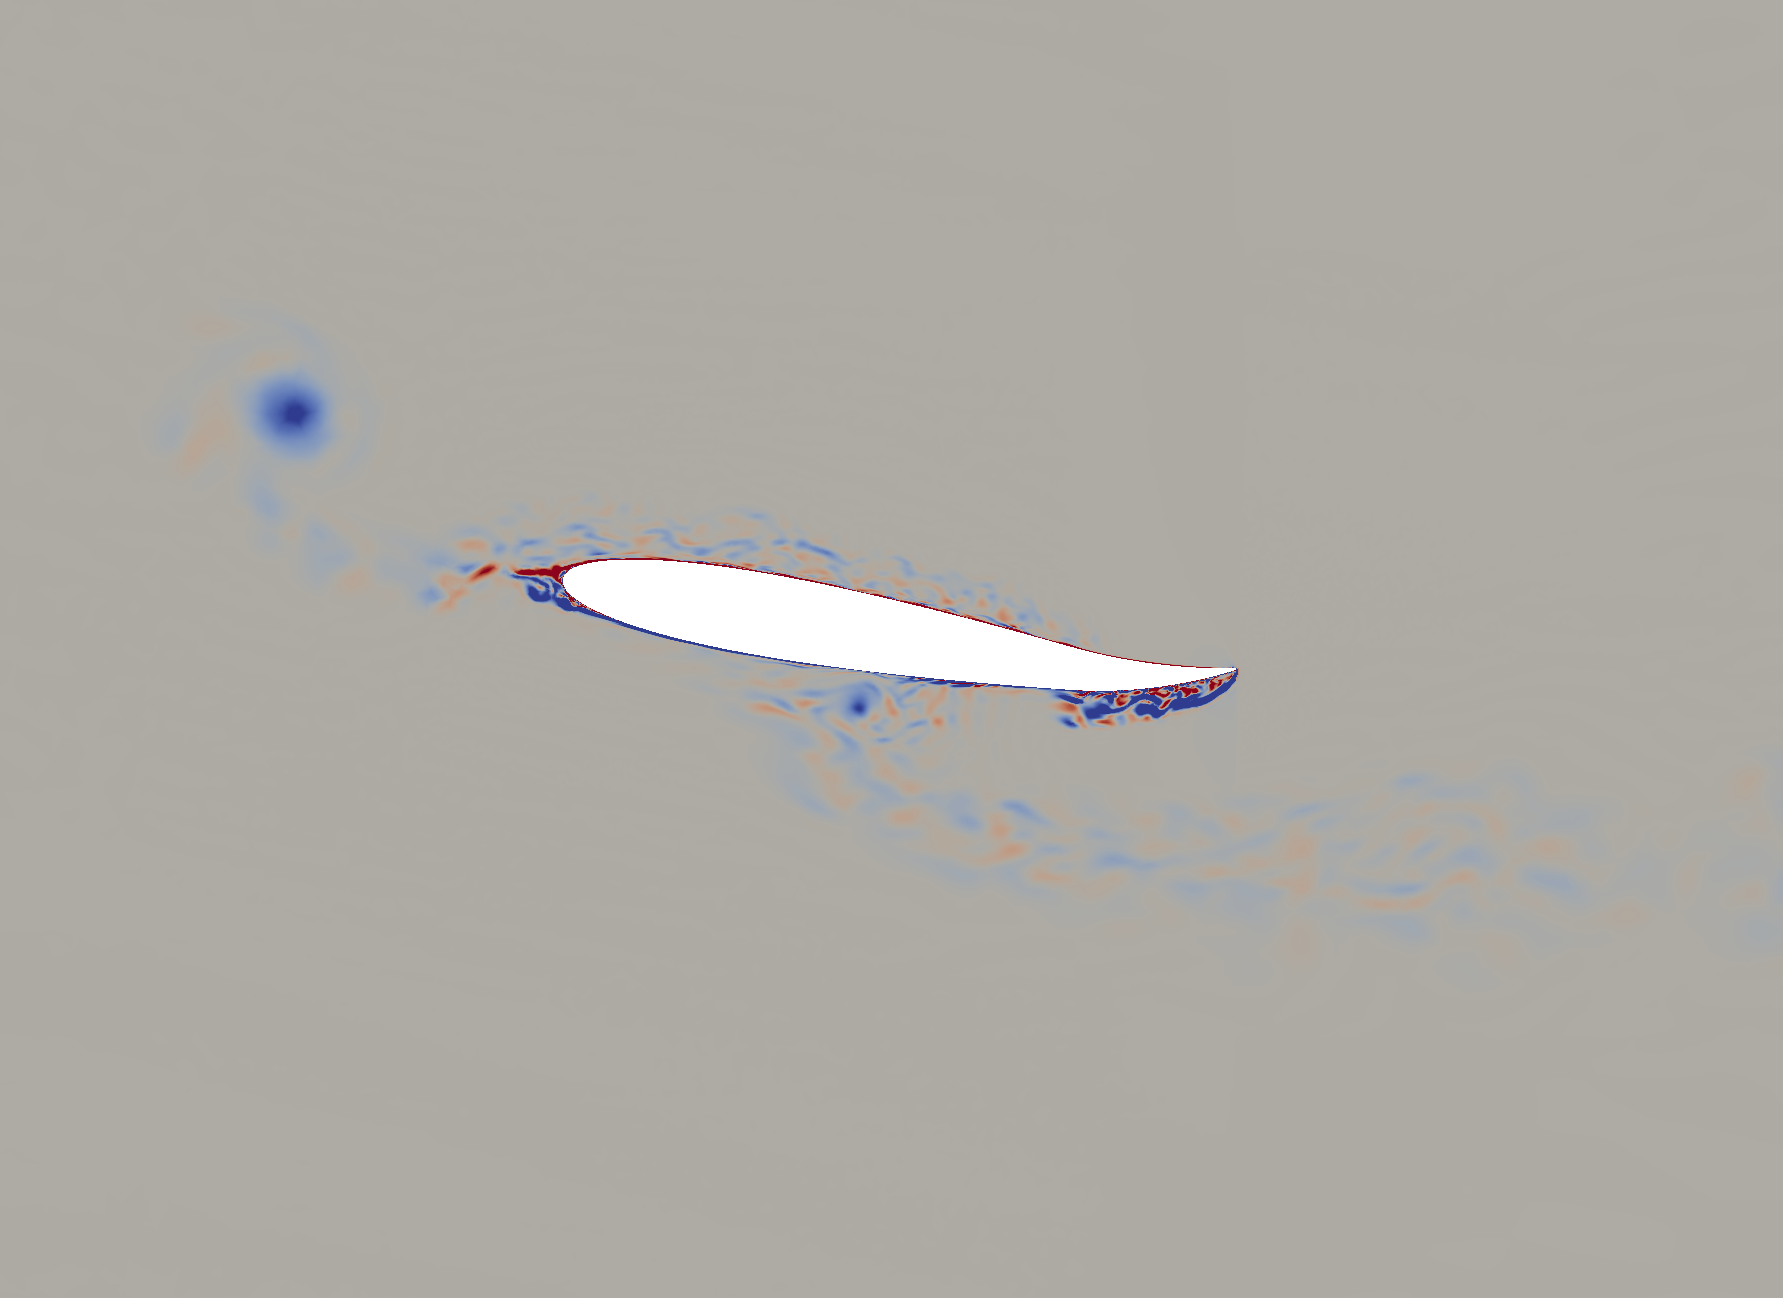
\includegraphics[width=1\textwidth]{figures/mu_1pt5/vorticity/AC/phase_255.png}
		\caption{ $\psi$ = $255^\circ$, $\tilde{t}=0.708$}
		\label{fig:mu_1pt5_AC_psi255}
	\end{subfigure}
	
	
	\caption{Instantaneous spanwise vorticity at 8 different phases for the baseline (left column) and actuated (right column) cases at $\mu_{sect}$ = 1.5}
	%\label{fig:vortScreen_mu1pt5}
\end{figure}

\begin{figure}[H]\ContinuedFloat
	\centering
	
	\begin{subfigure}[b]{0.4\textwidth}
		\centering
		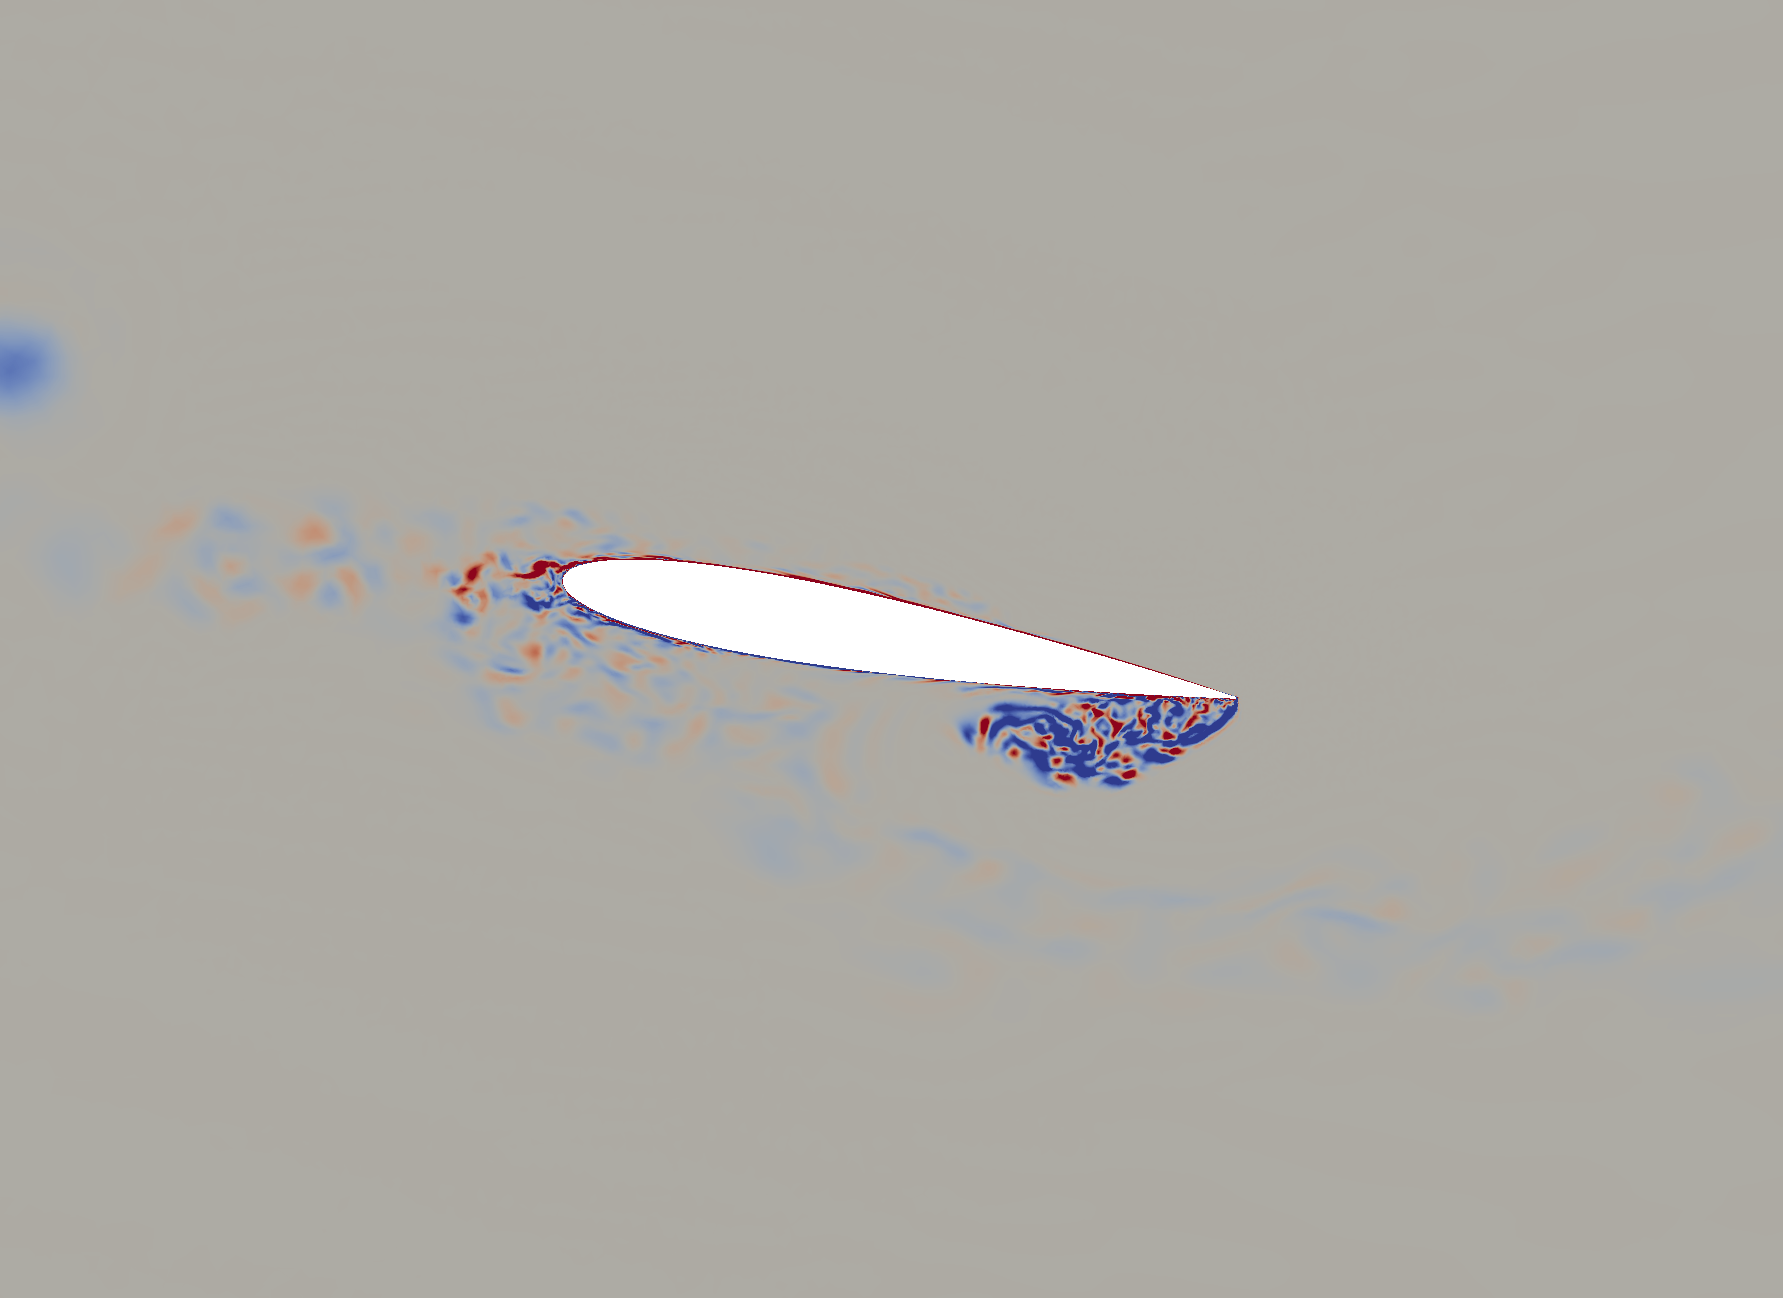
\includegraphics[width=1\textwidth]{figures/mu_1pt5/vorticity/baseline/phase_270.png}
		\caption{ $\psi$ = $270^\circ$, $\tilde{t}=0.75$}
		\label{fig:mu_1pt5_baseline_psi270}
	\end{subfigure}
	\begin{subfigure}[b]{0.4\textwidth}
		\centering
		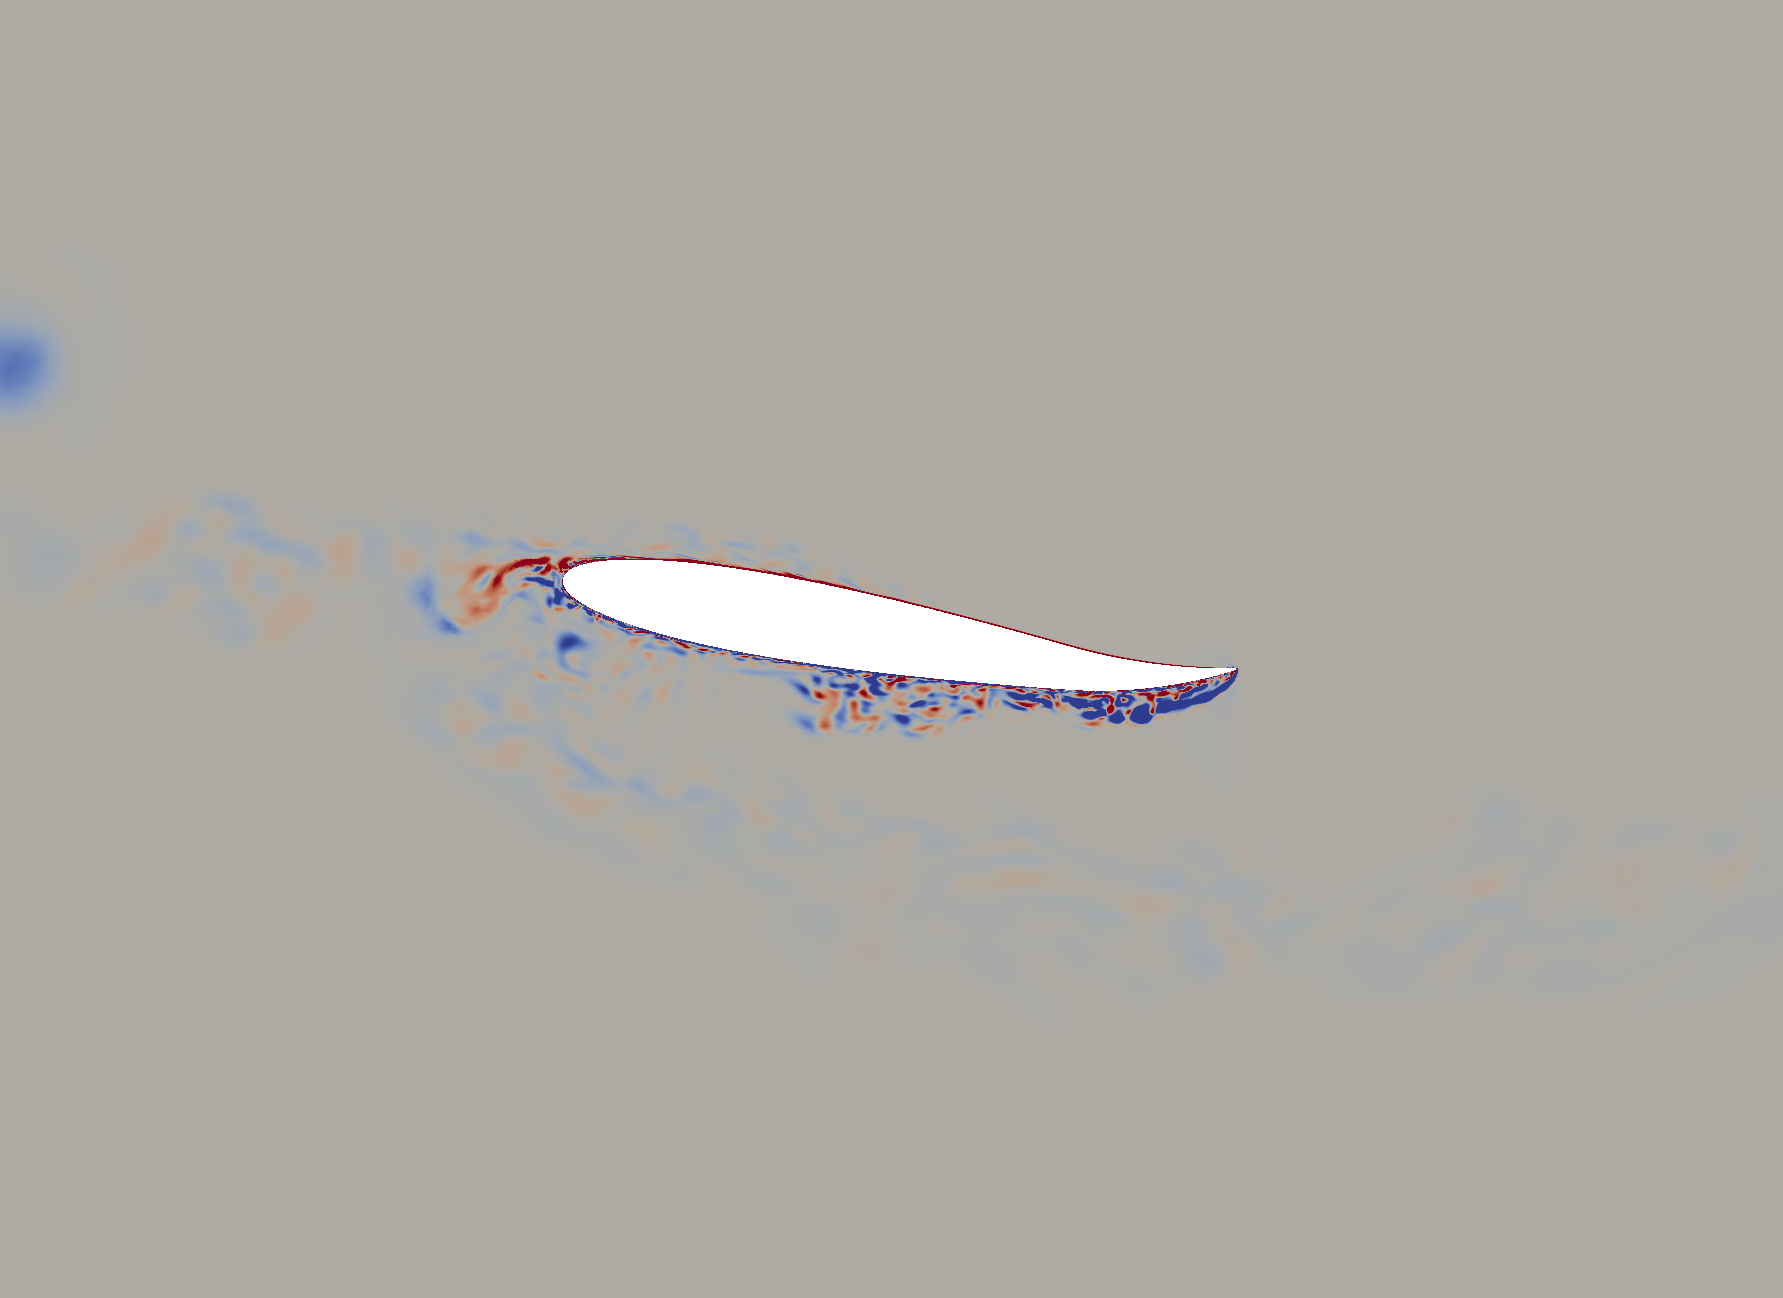
\includegraphics[width=1\textwidth]{figures/mu_1pt5/vorticity/AC/phase_270.png}
		\caption{ $\psi$ = $270^\circ$, $\tilde{t}=0.75$}
		\label{fig:mu_1pt5_AC_psi270}
	\end{subfigure}
	
	\begin{subfigure}[b]{0.4\textwidth}
		\centering
		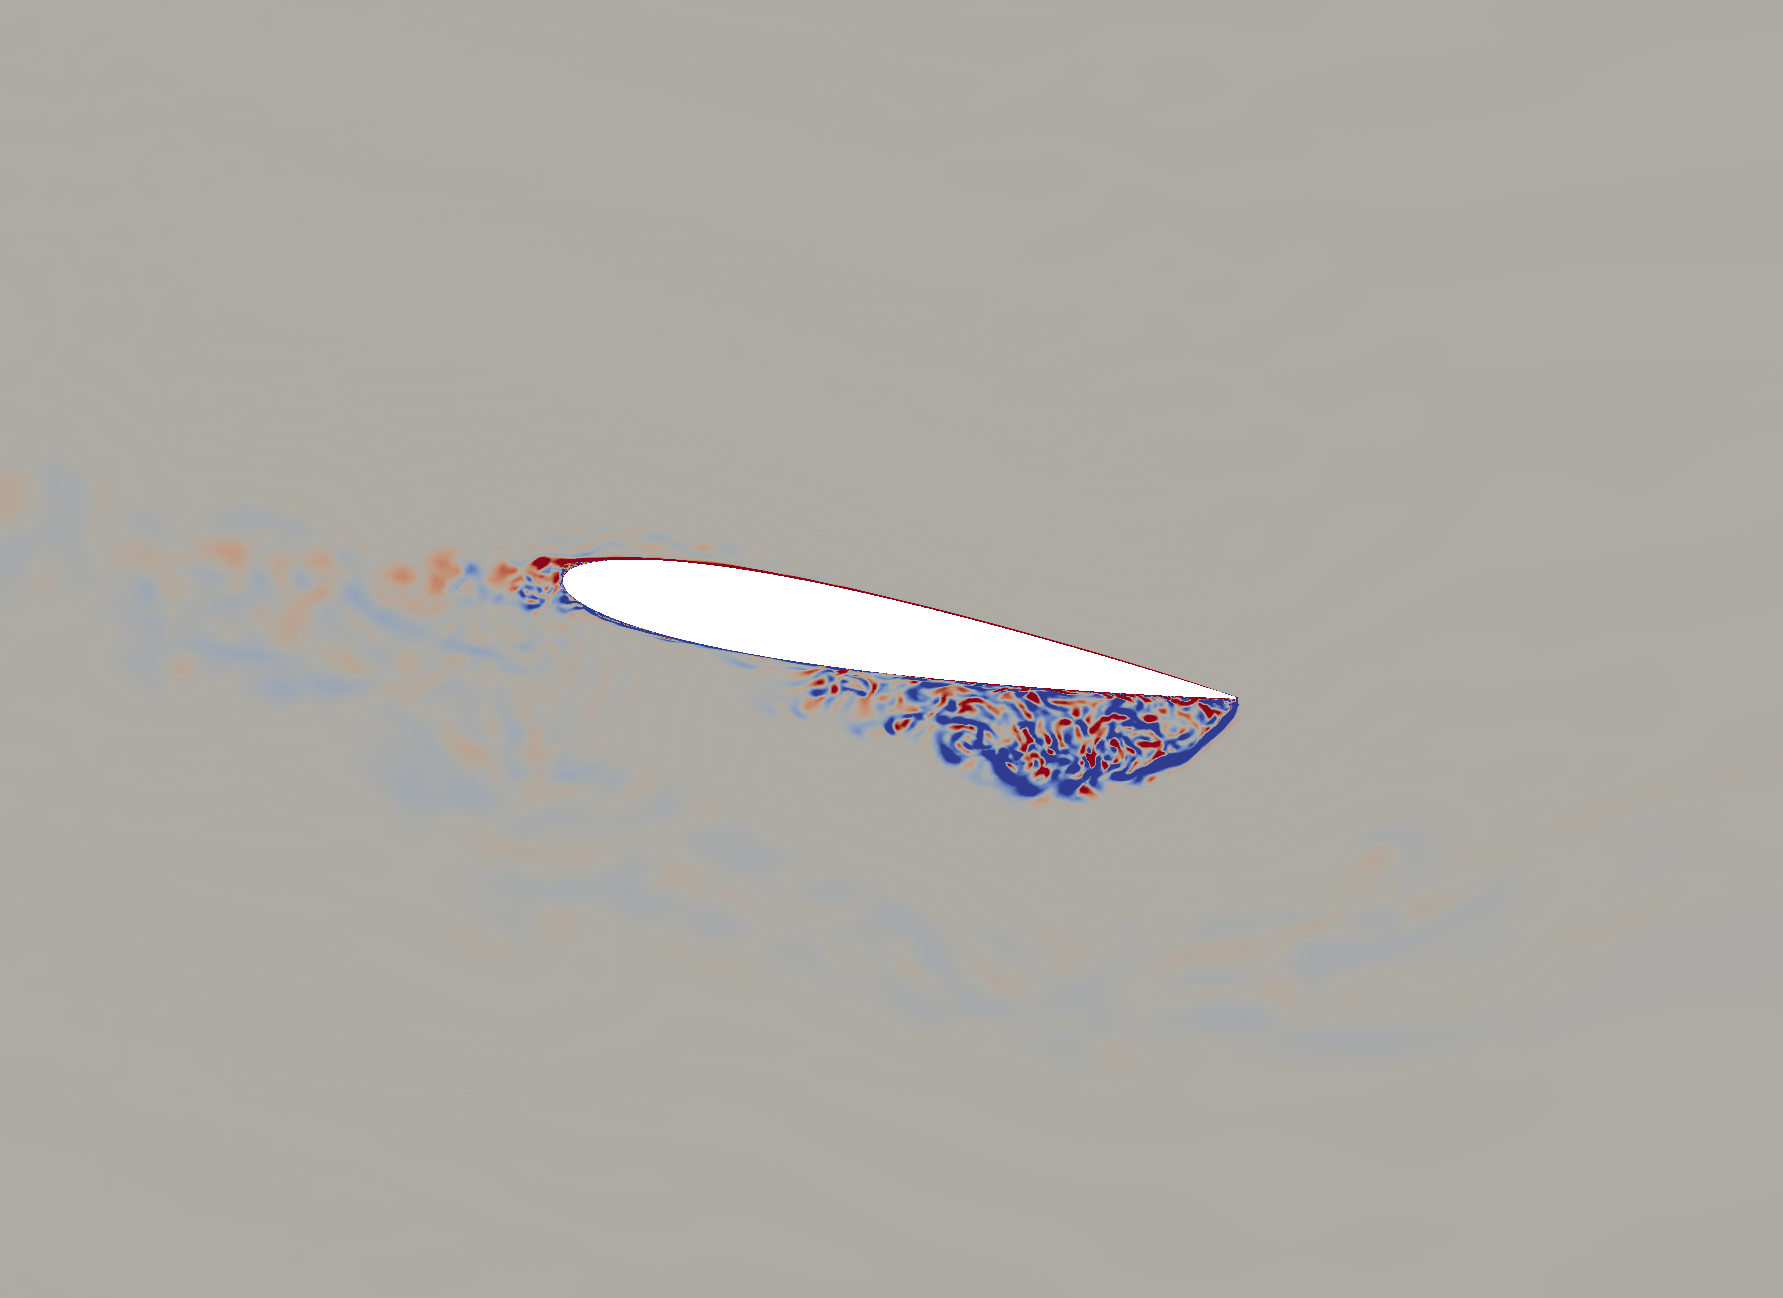
\includegraphics[width=1\textwidth]{figures/mu_1pt5/vorticity/baseline/phase_285.png}
		\caption{ $\psi$ = $285^\circ$, $\tilde{t}=0.792$}
		\label{fig:mu_1pt5_baseline_psi285}
	\end{subfigure}
	\begin{subfigure}[b]{0.4\textwidth}
		\centering
		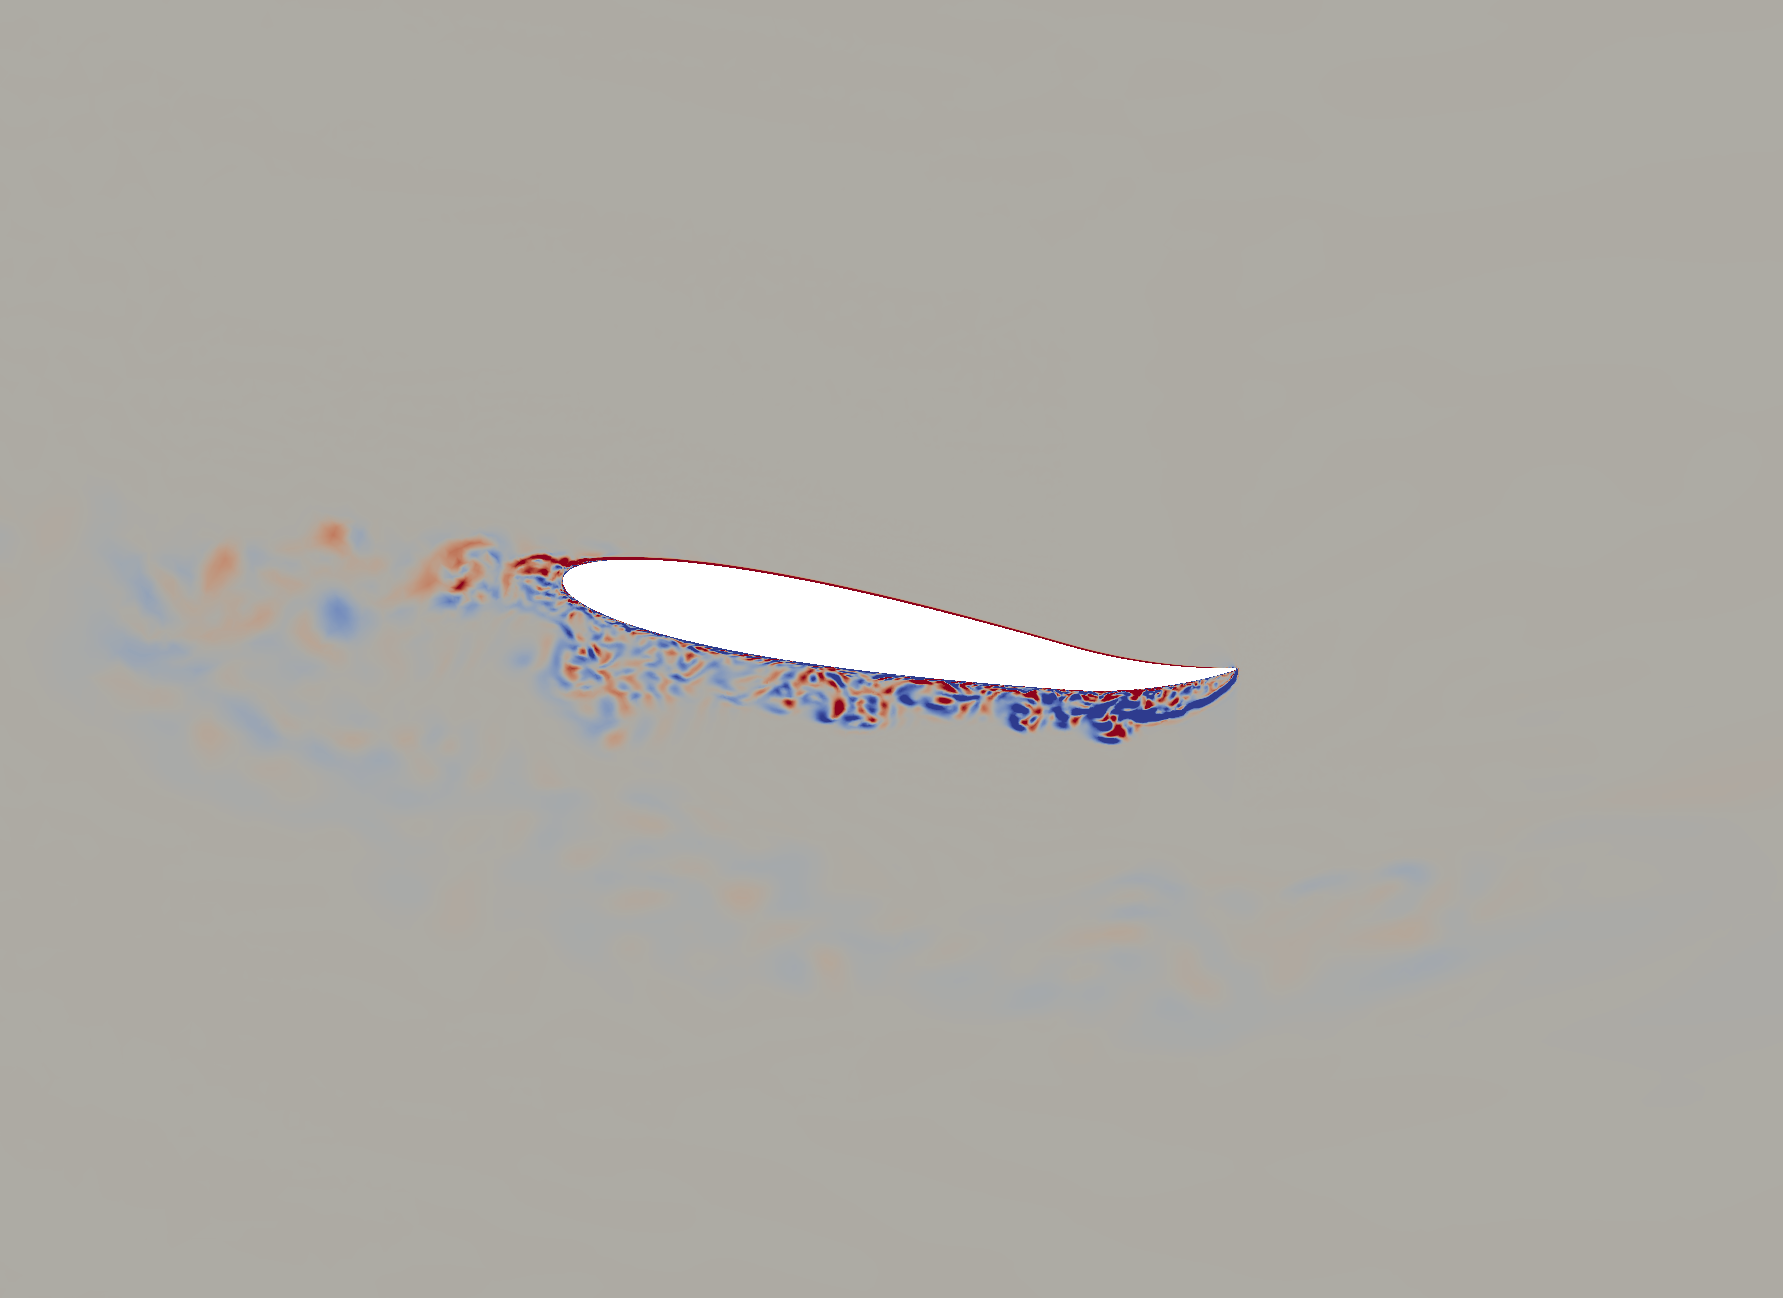
\includegraphics[width=1\textwidth]{figures/mu_1pt5/vorticity/AC/phase_285.png}
		\caption{ $\psi$ = $285^\circ$,  $\tilde{t}=0.792$}
		\label{fig:mu_1pt5_AC_psi285}
	\end{subfigure}
	
	
	%\begin{subfigure}[b]{0.4\textwidth}
	%	\centering
	%	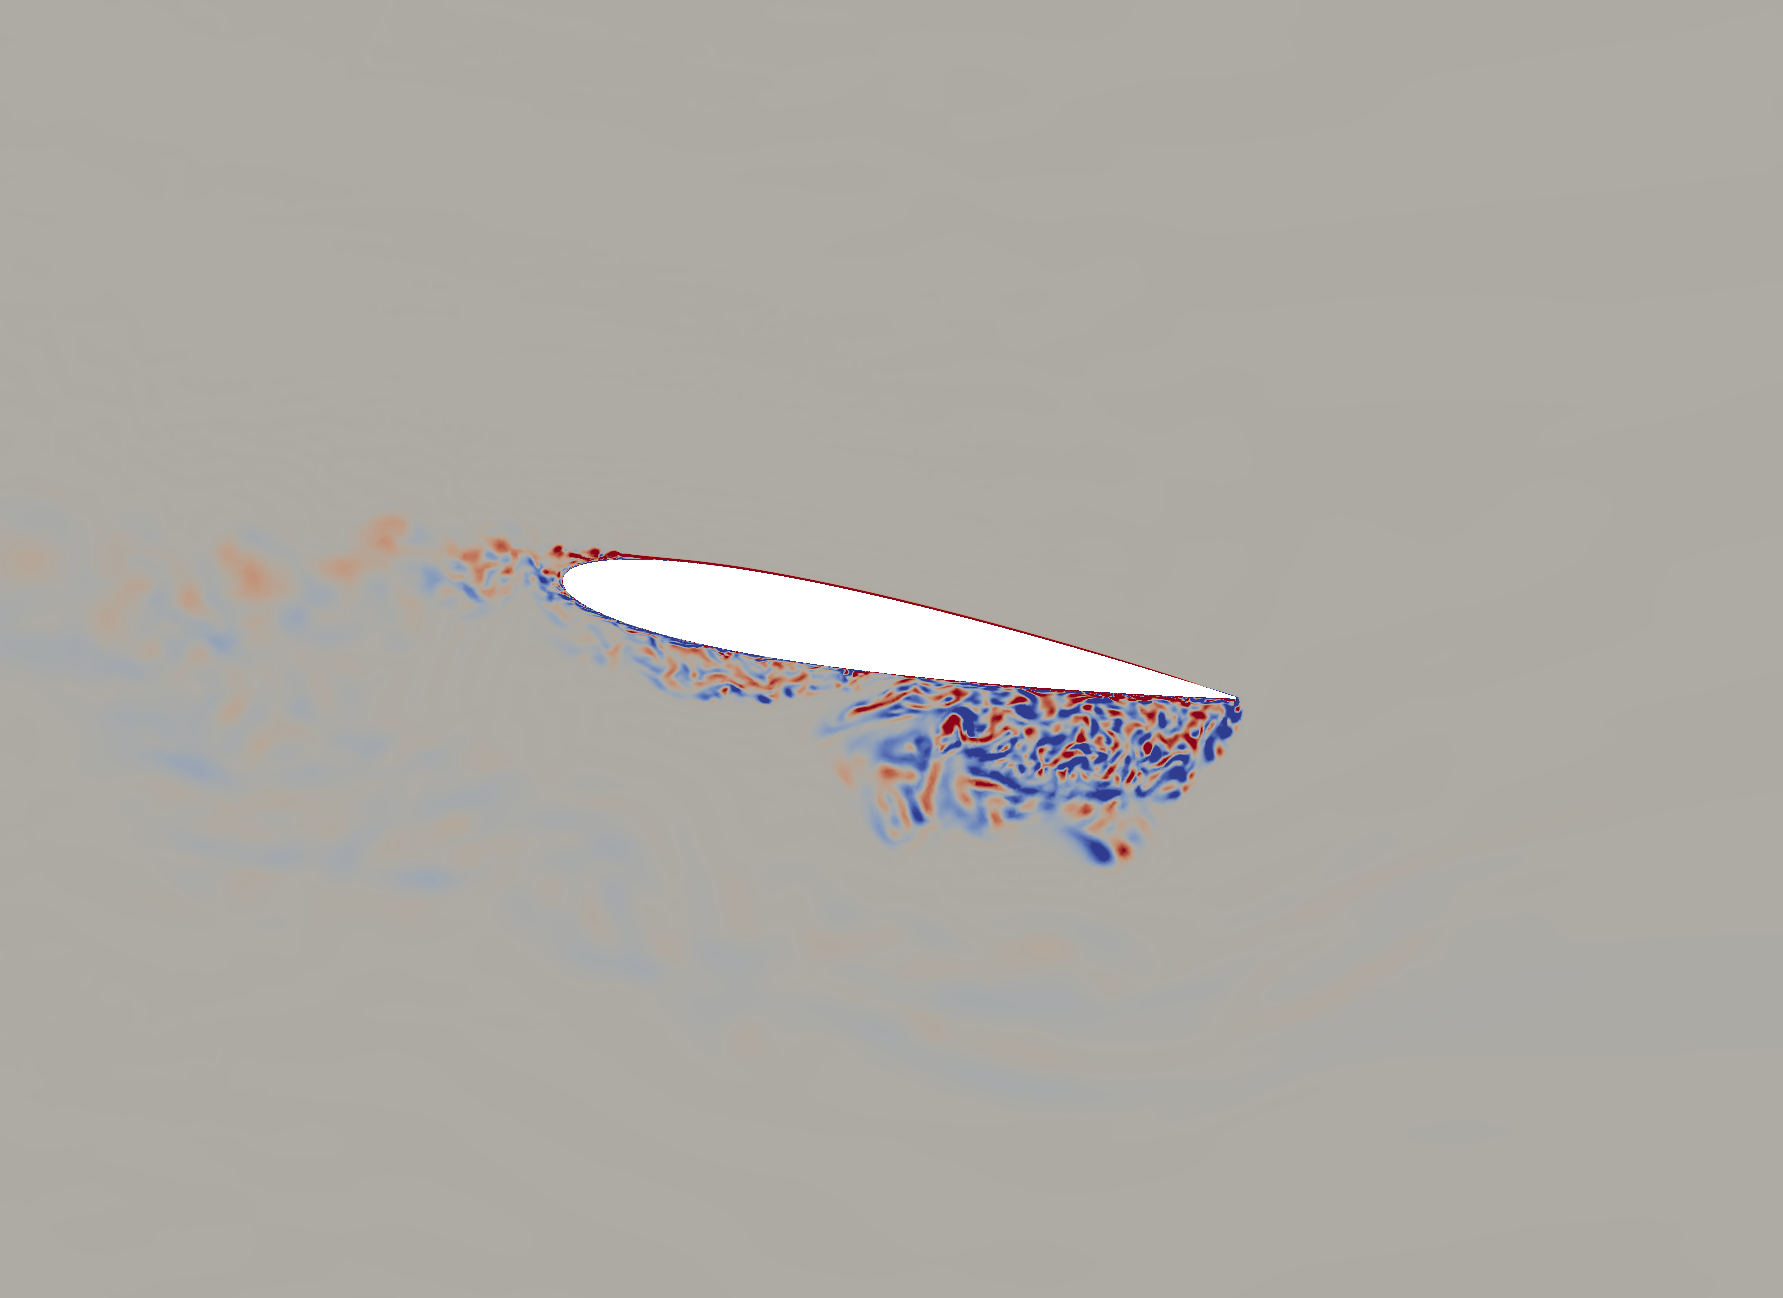
\includegraphics[width=1\textwidth]{figures/mu_1pt5/vorticity/baseline/phase_300.png}
	%	\caption{ $\psi$ = $300^\circ$, $\tilde{t}=0.833$}
	%	\label{fig:mu_1pt5_baseline_psi300}
	%\end{subfigure}
	%\begin{subfigure}[b]{0.4\textwidth}
	%	\centering
	%	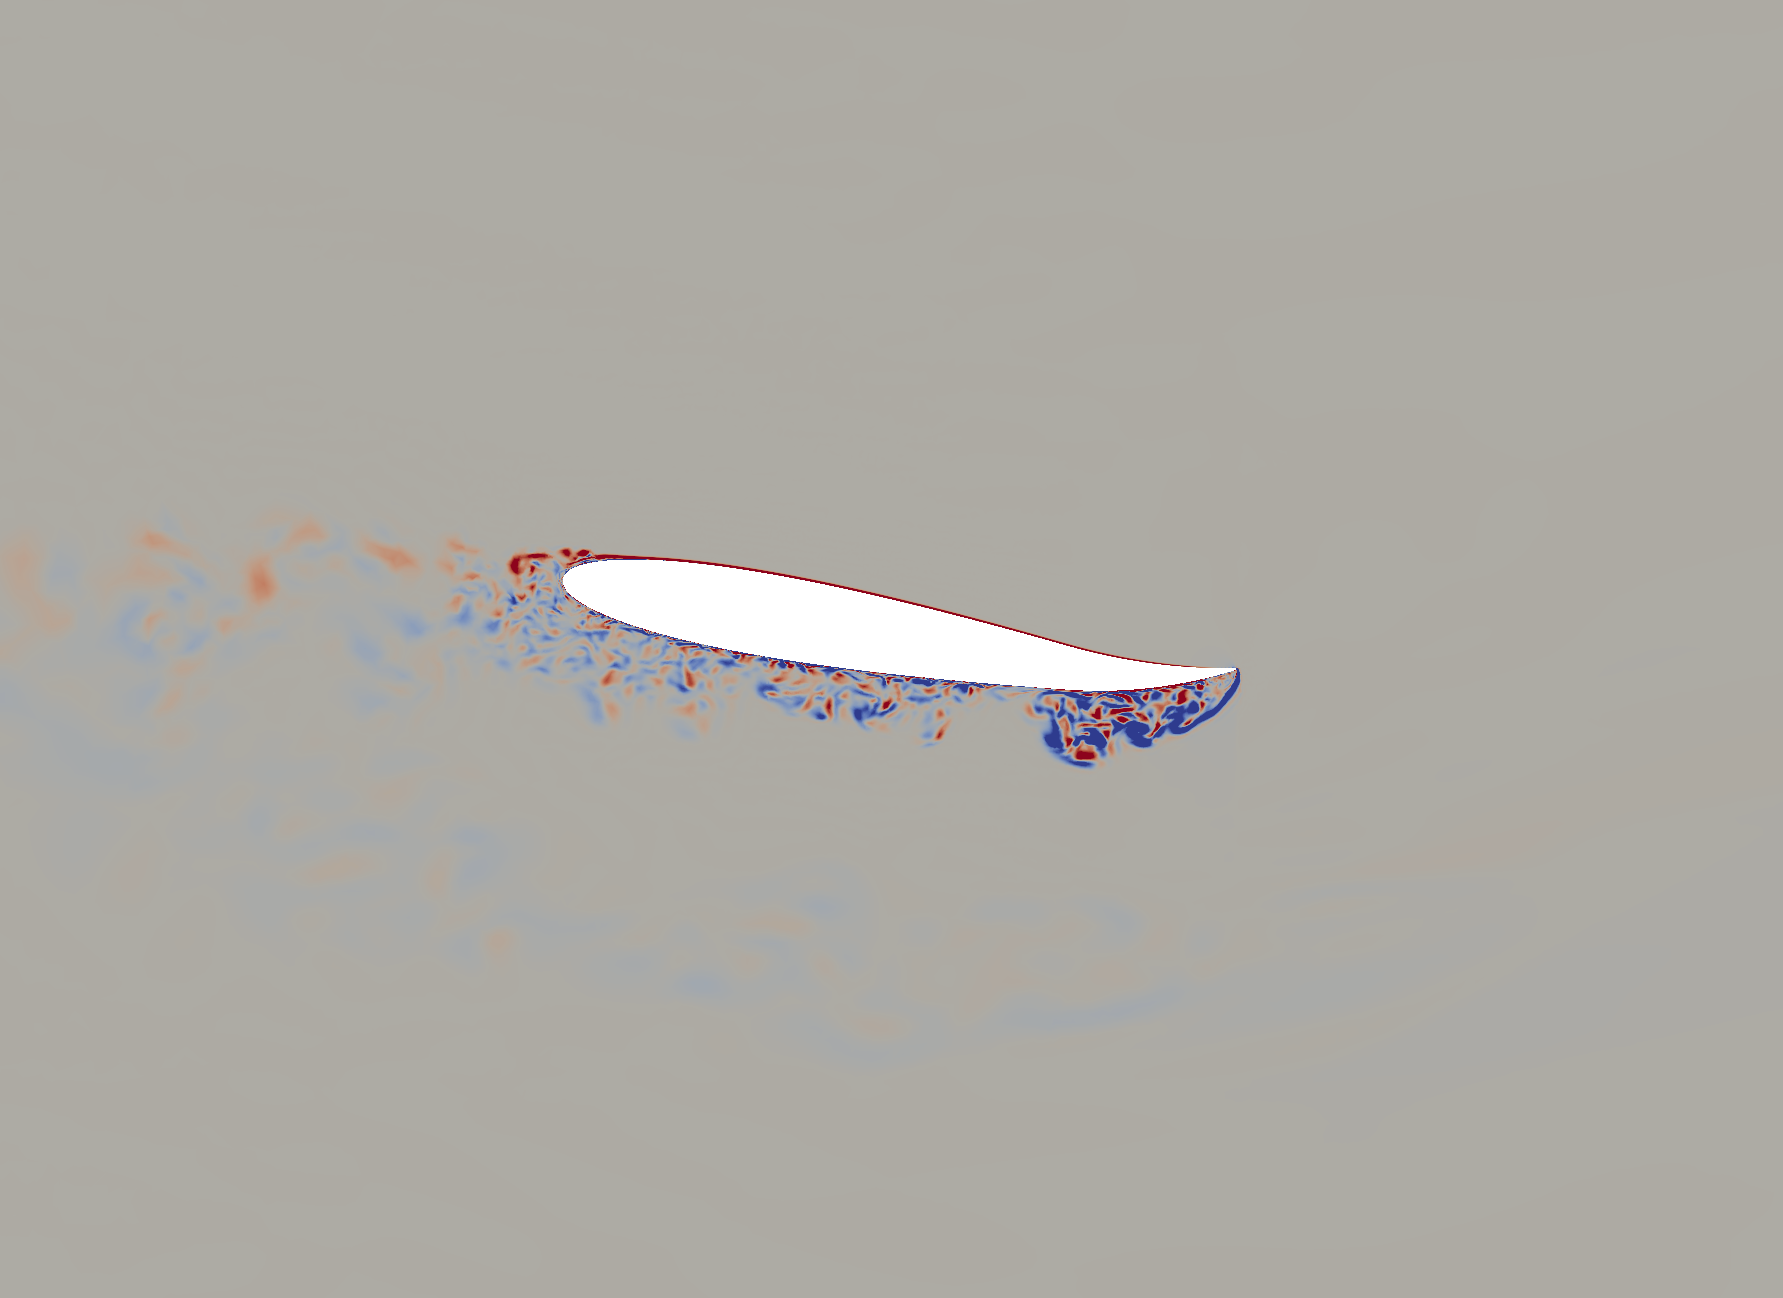
\includegraphics[width=1\textwidth]{figures/mu_1pt5/vorticity/AC/phase_300.png}
	%	\caption{ $\psi$ = $300^\circ$, $\tilde{t}=0.833$}
	%	\label{fig:mu_1pt5_AC_psi300}
	%\end{subfigure}
	
	\begin{subfigure}[b]{0.4\textwidth}
		\centering
		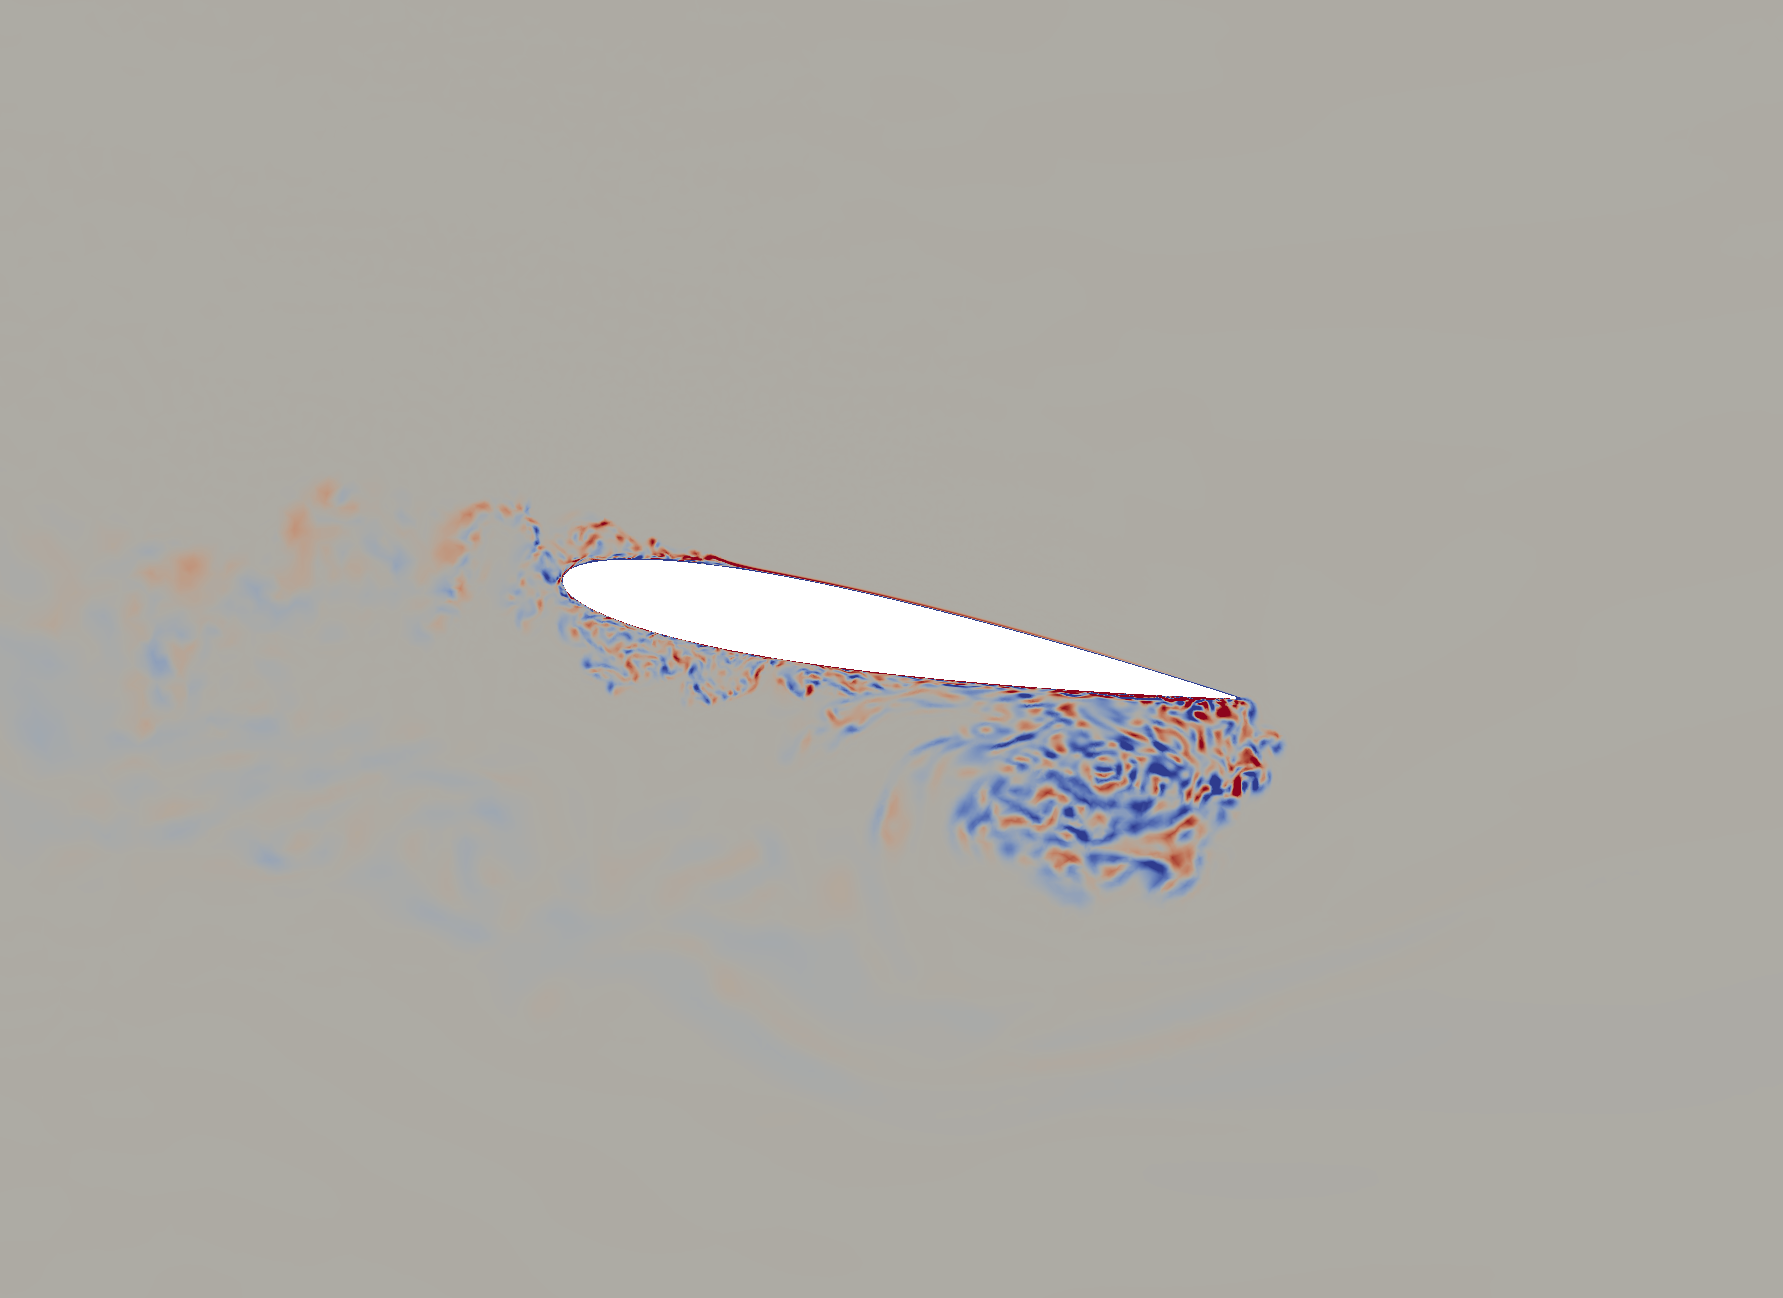
\includegraphics[width=1\textwidth]{figures/mu_1pt5/vorticity/baseline/phase_315.png}
		\caption{ $\psi$ = $315^\circ$, $\tilde{t}=0.875$}
		\label{fig:mu_1pt5_baseline_psi315}
	\end{subfigure}
	\begin{subfigure}[b]{0.4\textwidth}
		\centering
		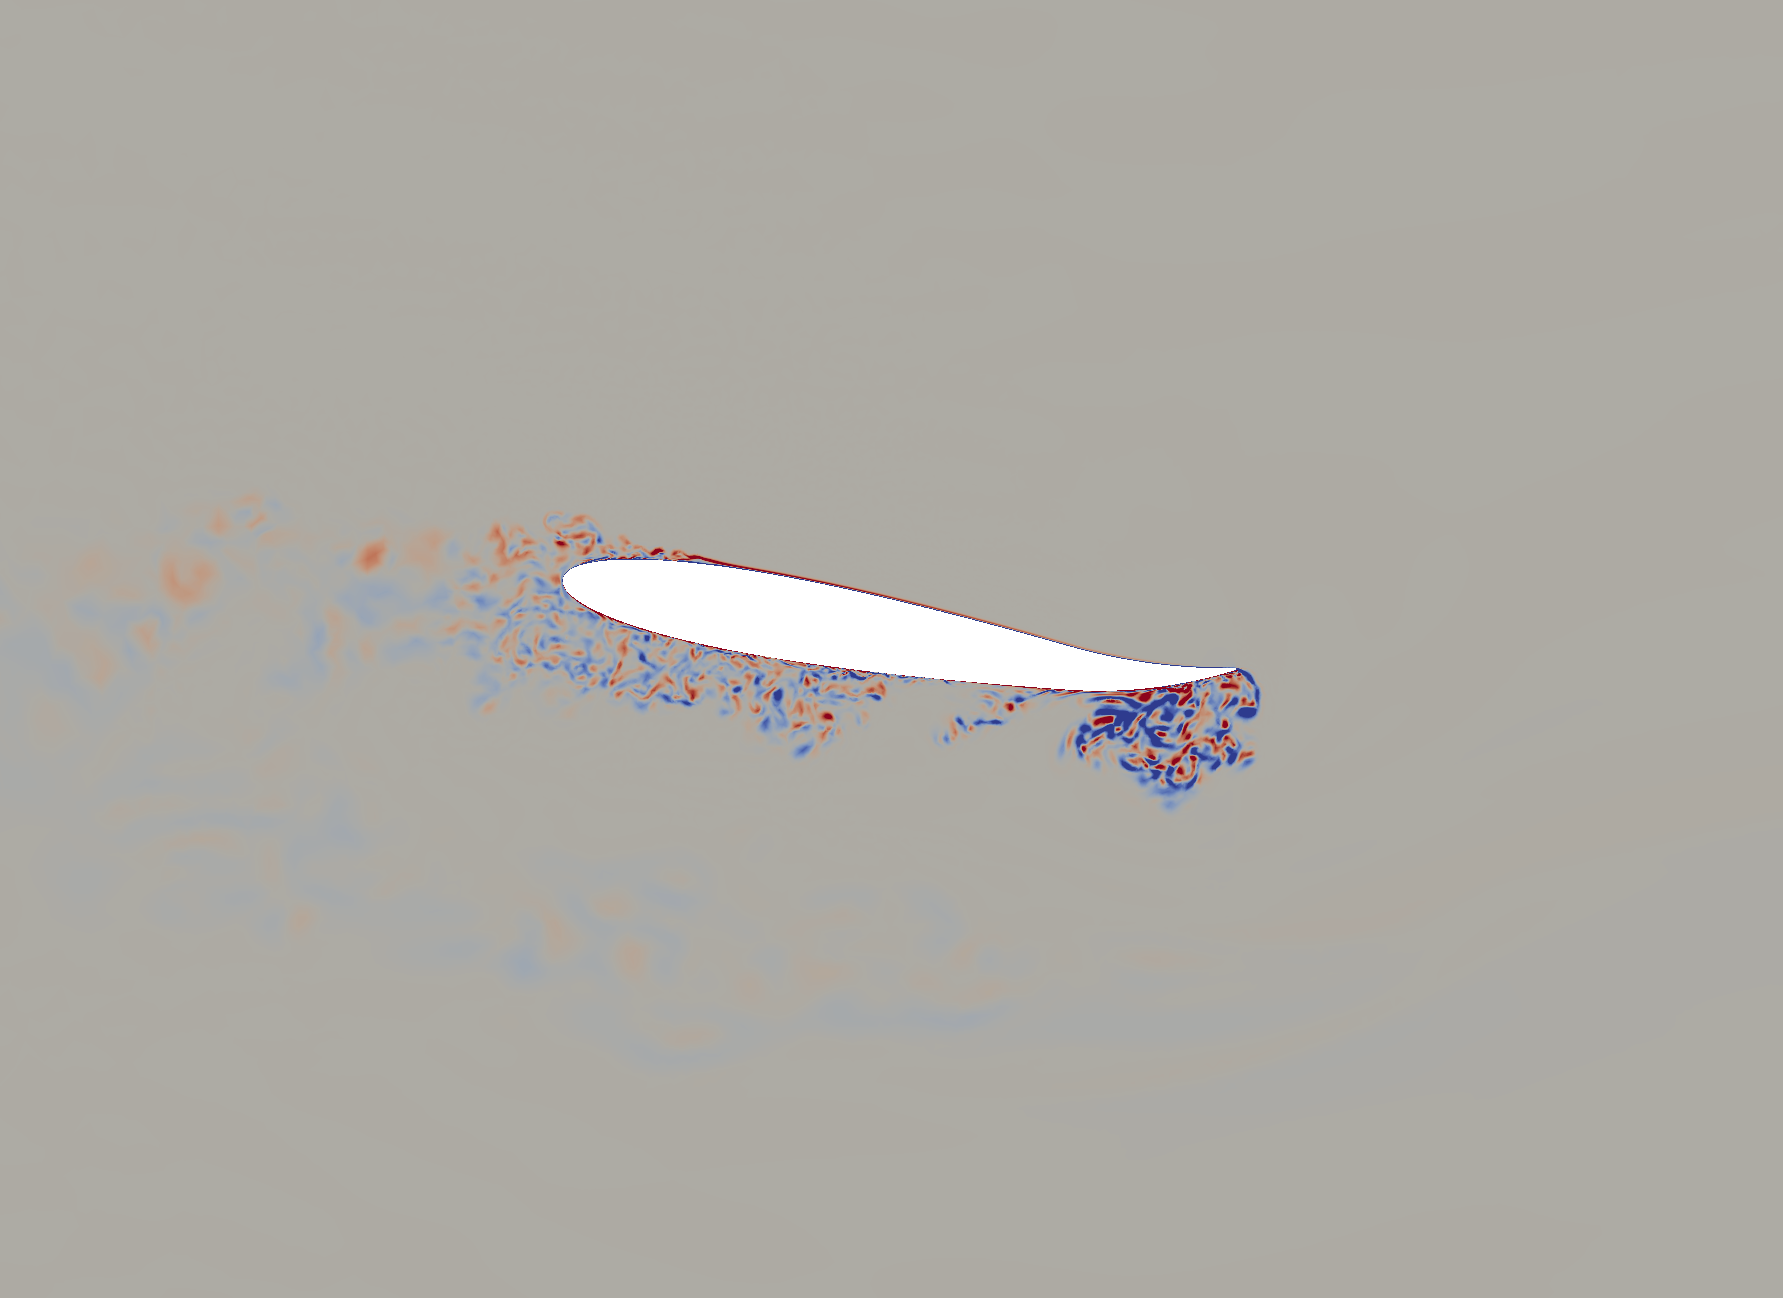
\includegraphics[width=1\textwidth]{figures/mu_1pt5/vorticity/AC/phase_315.png}
		\caption{ $\psi$ = $315^\circ$, $\tilde{t}=0.875$}
		\label{fig:mu_1pt5_AC_psi315}
	\end{subfigure}
	
	\begin{subfigure}[b]{0.4\textwidth}
		\centering
		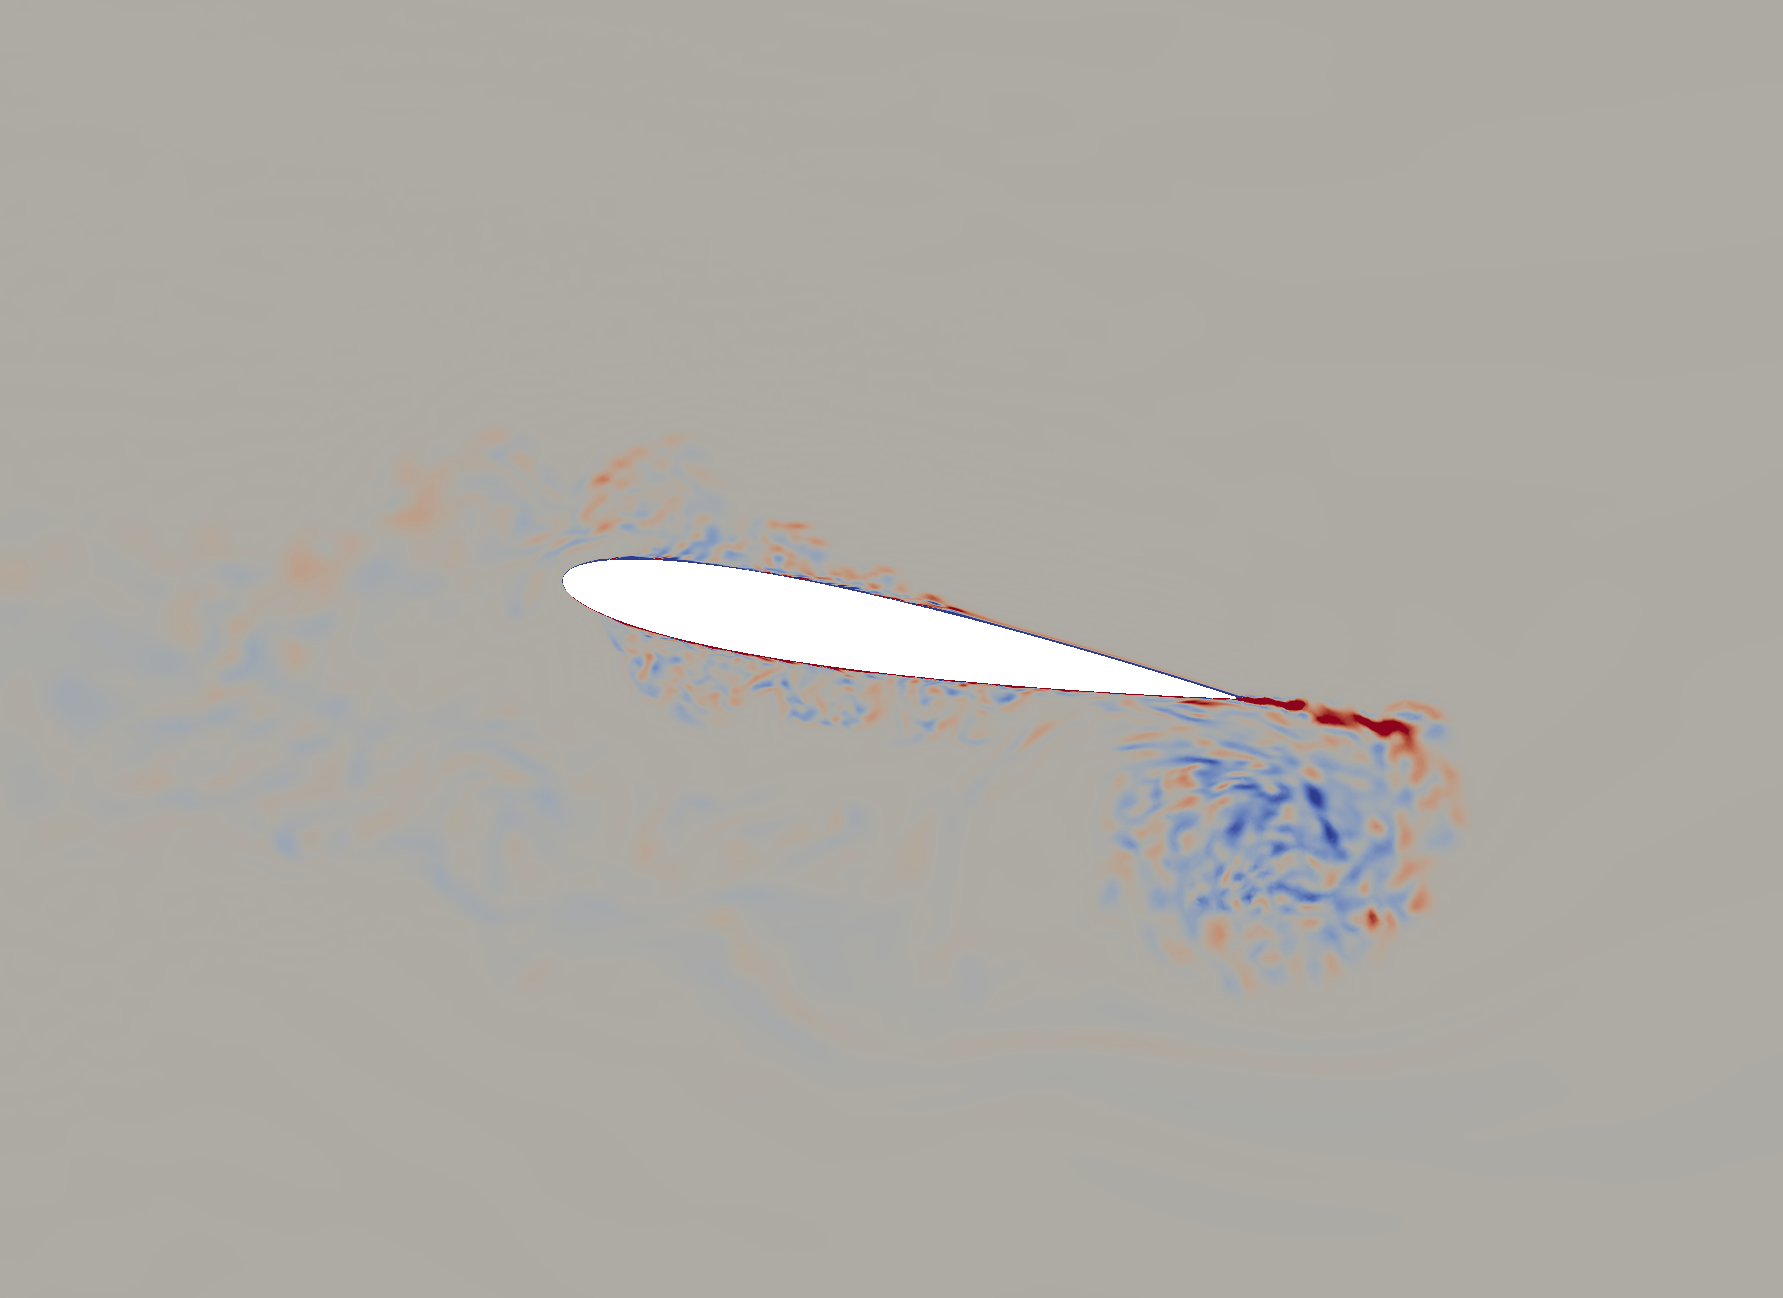
\includegraphics[width=1\textwidth]{figures/mu_1pt5/vorticity/baseline/phase_330.png}
		\caption{ $\psi$ = $330^\circ$, $\tilde{t}=0.917$}
		\label{fig:mu_1pt5_baseline_psi330}
	\end{subfigure}
	\begin{subfigure}[b]{0.4\textwidth}
		\centering
		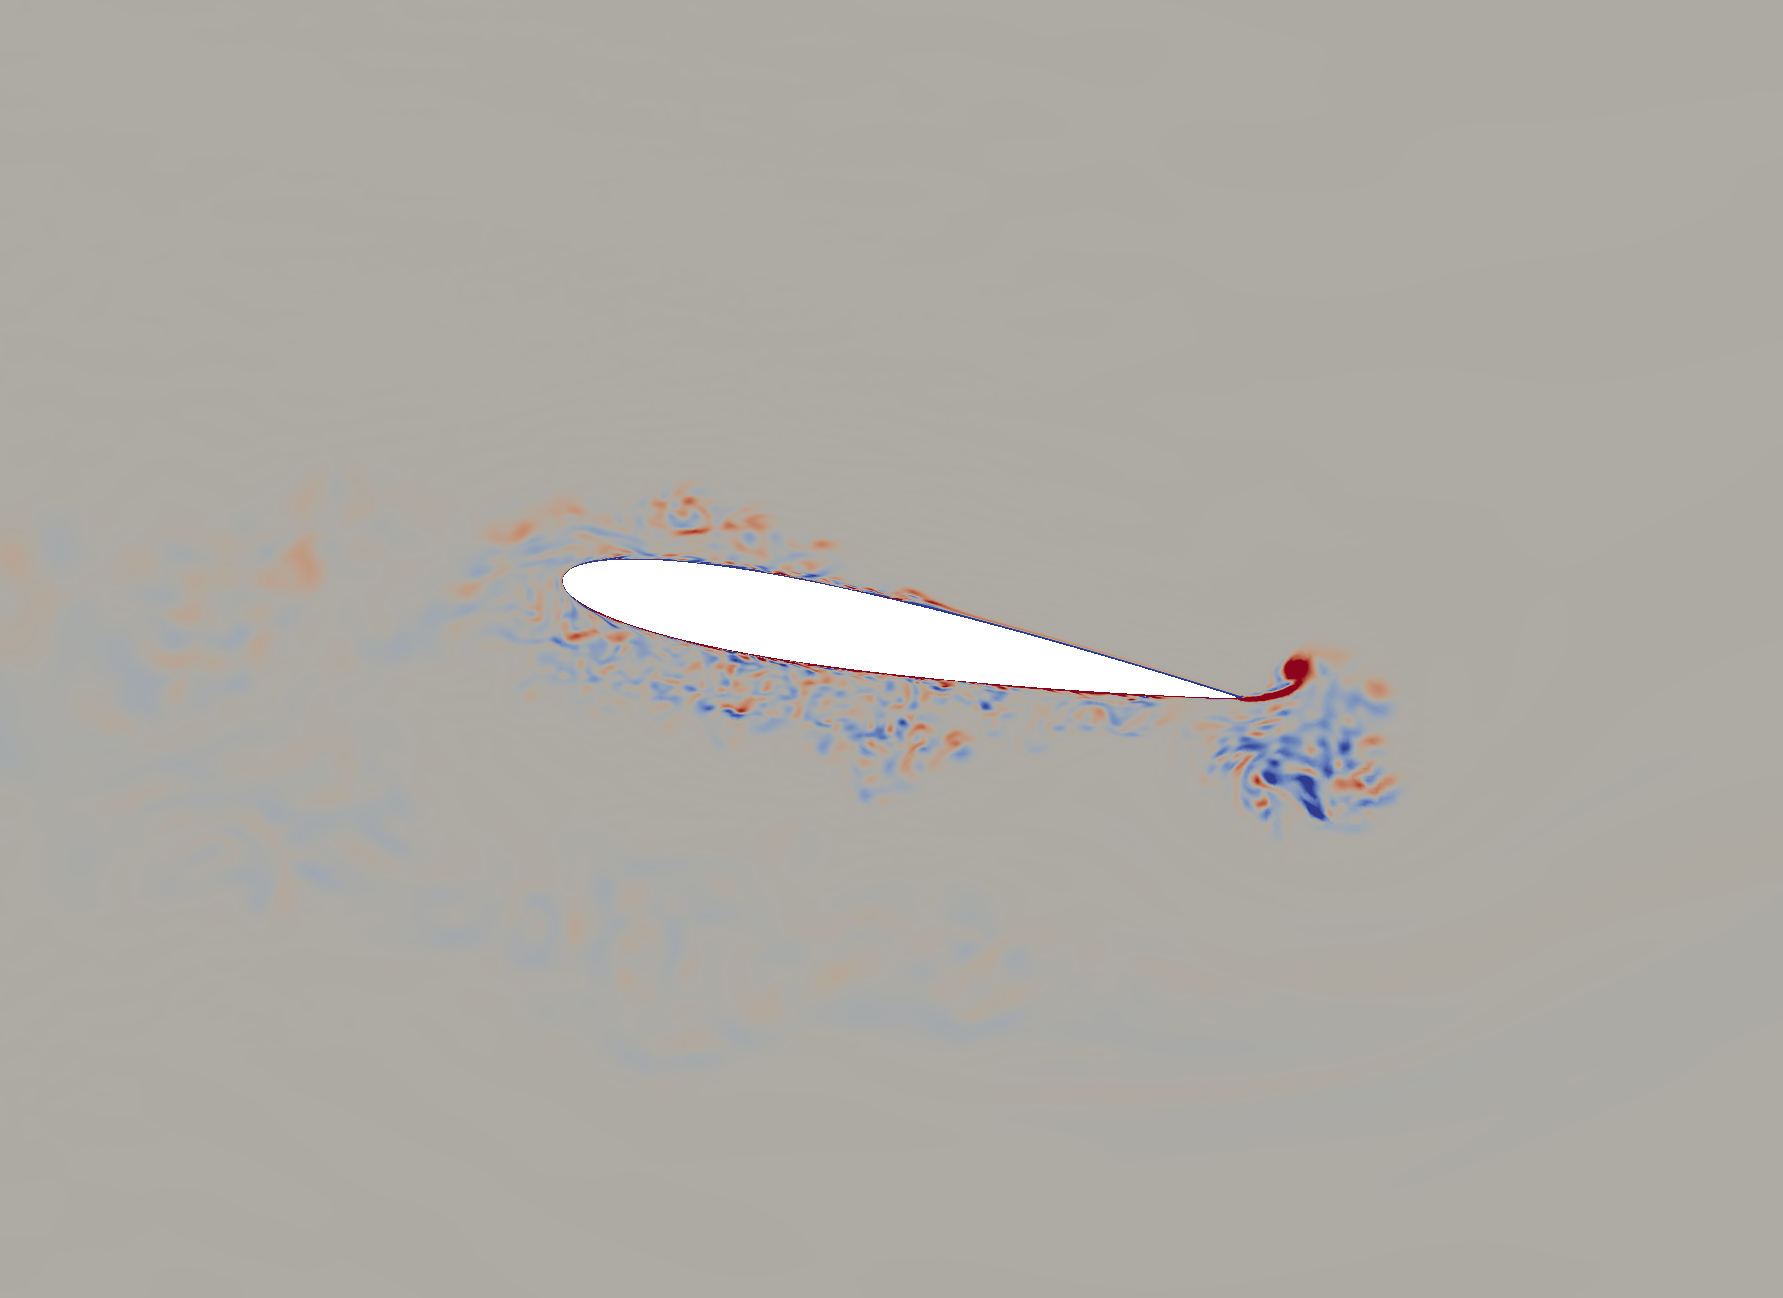
\includegraphics[width=1\textwidth]{figures/mu_1pt5/vorticity/AC/phase_330.png}
		\caption{ $\psi$ = $330^\circ$, $\tilde{t}=0.917$}
		\label{fig:mu_1pt5_AC_psi330}
	\end{subfigure}
	
	%\begin{subfigure}[b]{0.4\textwidth}
	%	\centering
	%	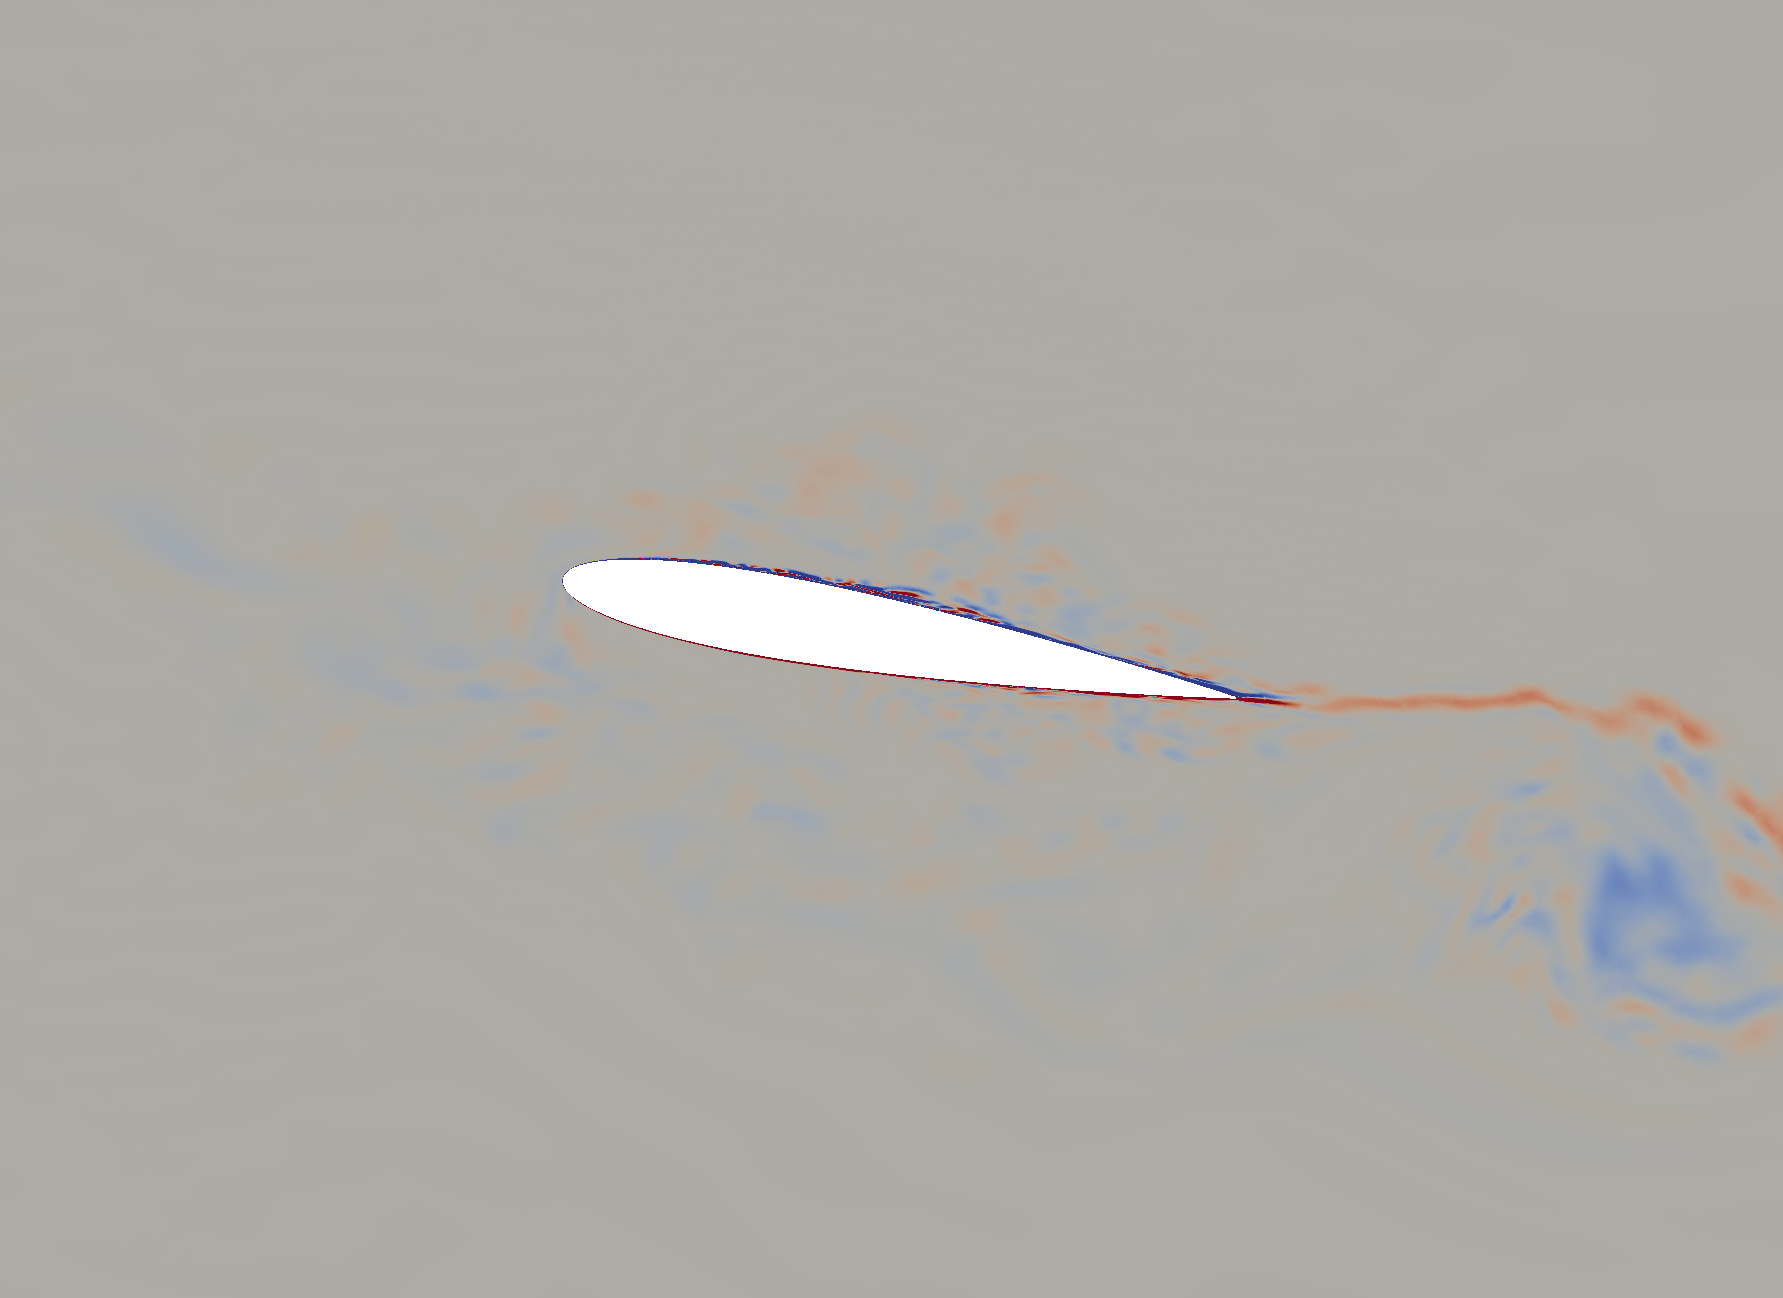
\includegraphics[width=1\textwidth]{figures/mu_1pt5/vorticity/baseline/phase_345.png}
	%	\caption{ $\psi$ = $345^\circ$, $\tilde{t}=0.958$}
	%	\label{fig:mu_1pt5_baseline_psi345}
	%\end{subfigure}
	%\begin{subfigure}[b]{0.4\textwidth}
	%	\centering
	%	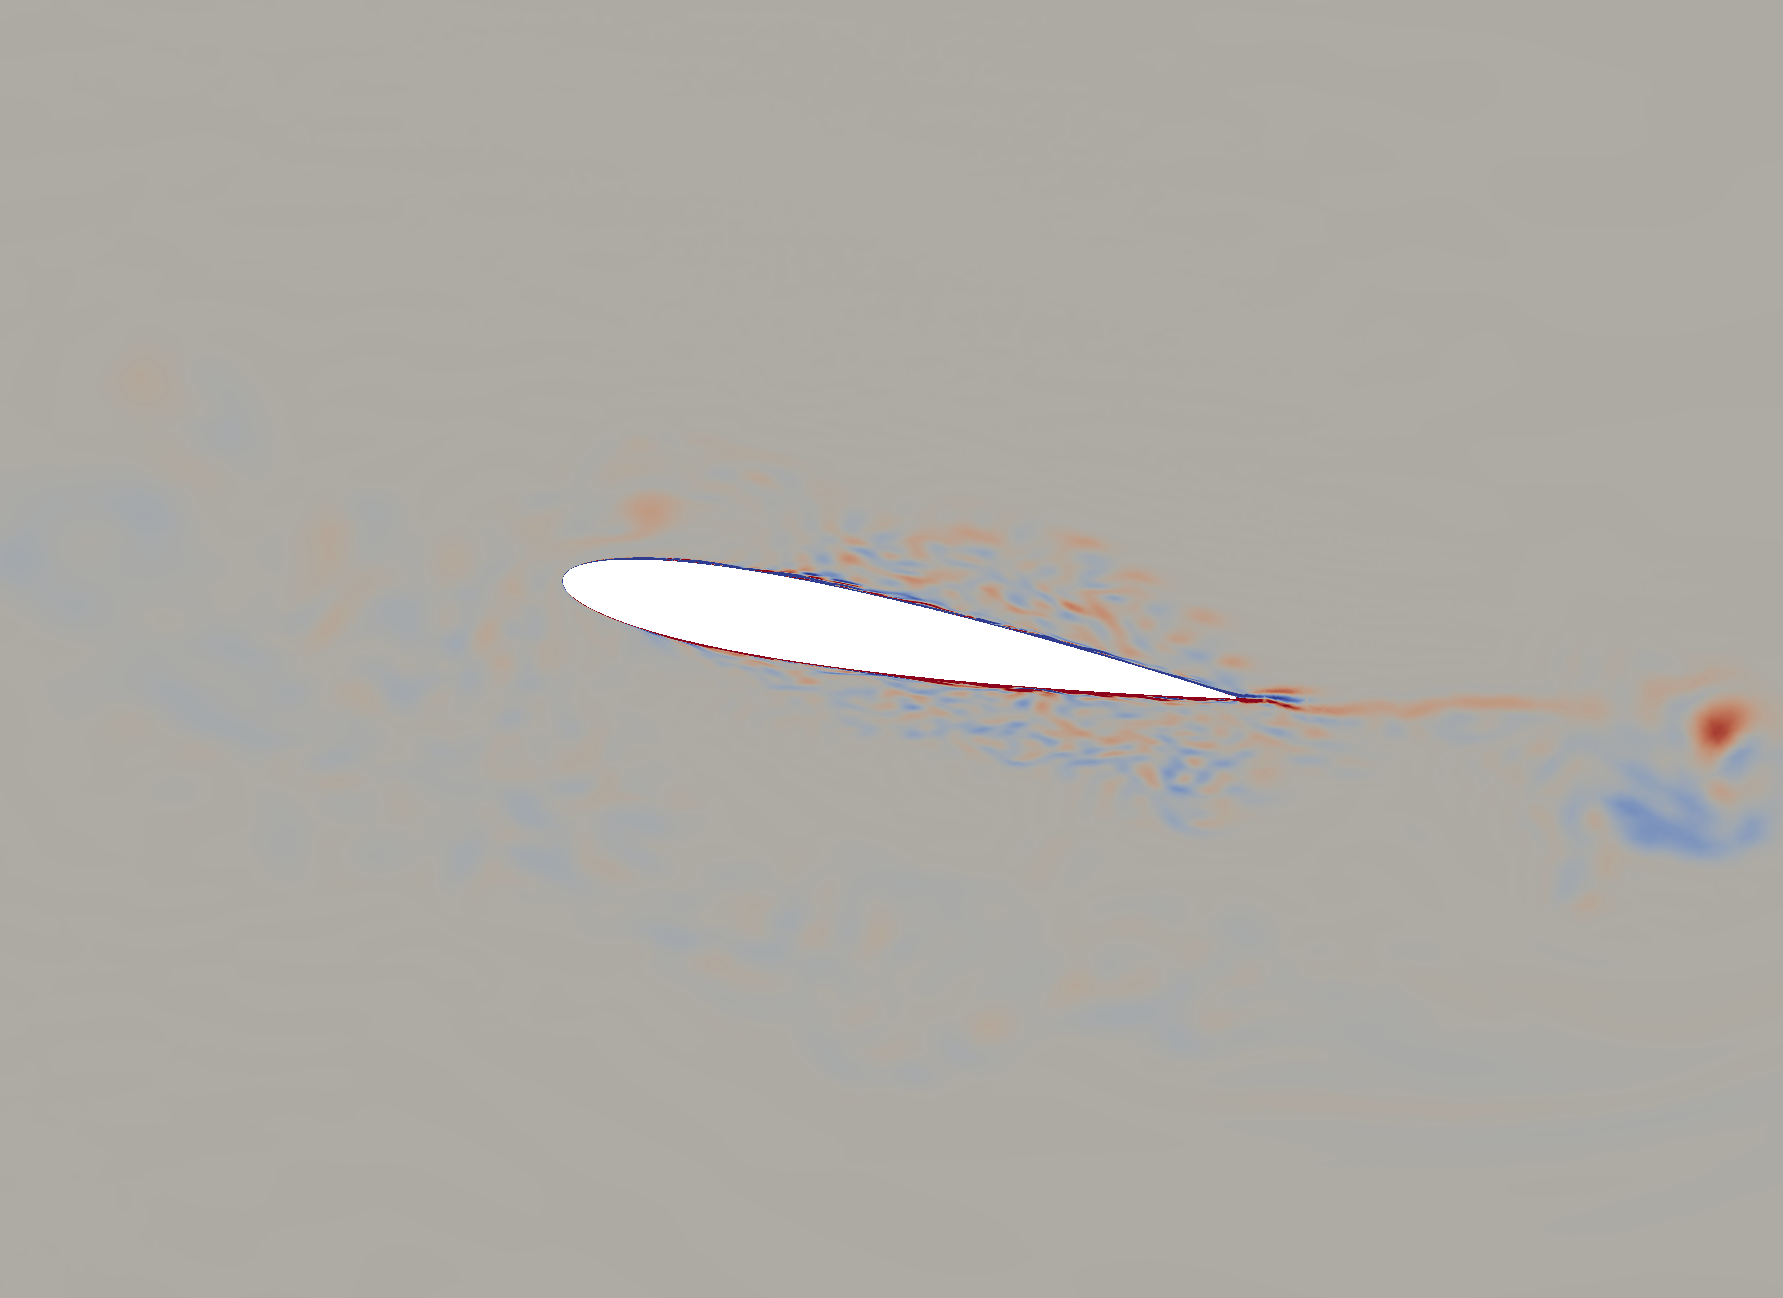
\includegraphics[width=1\textwidth]{figures/mu_1pt5/vorticity/AC/phase_345.png}
	%	\caption{ $\psi$ = $345^\circ$, $\tilde{t}=0.958$}
	%	\label{fig:mu_1pt5_AC_psi345}
	%\end{subfigure}
	
	
	
	\caption{Instantaneous spanwise vorticity at 8 different phases for the baseline (left column) and actuated (right column) cases at $\mu_{sect}$ = 1.5}
	\label{fig:vortScreen_mu1pt5}
\end{figure}

Figures \ref{fig:mu_1pt5_zoomed_velocity} and \ref{fig:mu_2pt0_zoomed_velocity} show a comparison of the instantaneous velocity magnitude in the vicinity of the trailing edge. Both baseline and actuated cases are shown at $\psi$ = $270^\circ$ (i.e., at the peak of reverse flow).
The corresponding spanwise vorticity plots are shown in Figures \ref{fig:mu_1pt5_zoomed_vorticity} and \ref{fig:mu_2pt0_zoomed_vorticity}.
Note that the flow velocity is with respect to the airfoil. 
The velocity magnitude range is selected to be [0,1.5]$ U_{sect}$.
The vorticity range is the same as before, [-30,30]$ U_{sect}/C$.

In both cases, the flow is highly turbulent (as clearly evident from the resolved turbulent flow structures by the current LES). 
In the baseline cases a large region of flow separation is observed while in the actuated cases this separated region is substantially smaller.
In the baseline case with $\mu_{sect}=2.0$ the separated region in the baseline case is larger as compared to that in the case with $\mu_{sect}=1.5$.
However, in the actuated cases the size of the separated region is very similar  between $\mu_{sect}=1.5$ and $2.0$, see Figures \ref{fig:mu_1pt5_AC_zoomed_velocity} and \ref{fig:mu_2pt0_AC_zoomed_velocity} as well as Figures \ref{fig:mu_1pt5_AC_zoomed_vorticity} and \ref{fig:mu_2pt0_AC_zoomed_vorticity}.

\begin{figure}[H]
	\centering
	
	\begin{subfigure}[b]{0.4\textwidth}
		\centering
		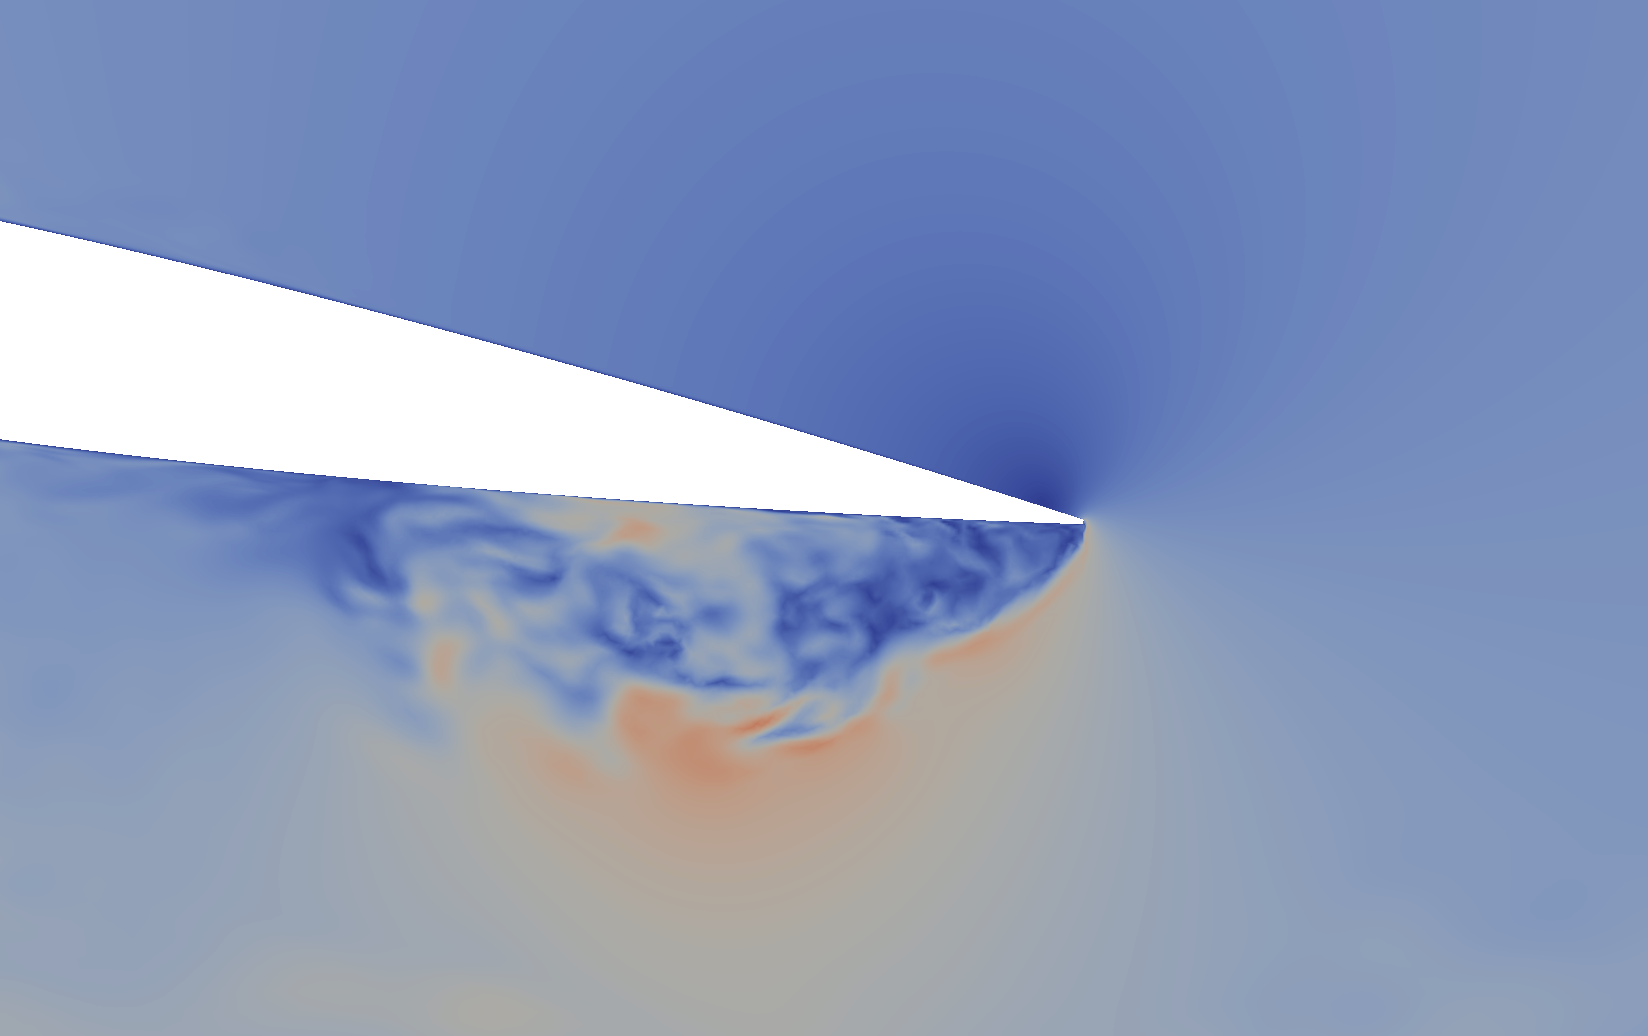
\includegraphics[width=1\textwidth]{figures/mu_1pt5/baseline/ph_270_velocity_zoomed_airfoil_0_to_1pt5.png}
		\caption{ baseline}
		\label{fig:mu_1pt5_baseline_zoomed_velocity}
	\end{subfigure}
	\begin{subfigure}[b]{0.4\textwidth}
		\centering
		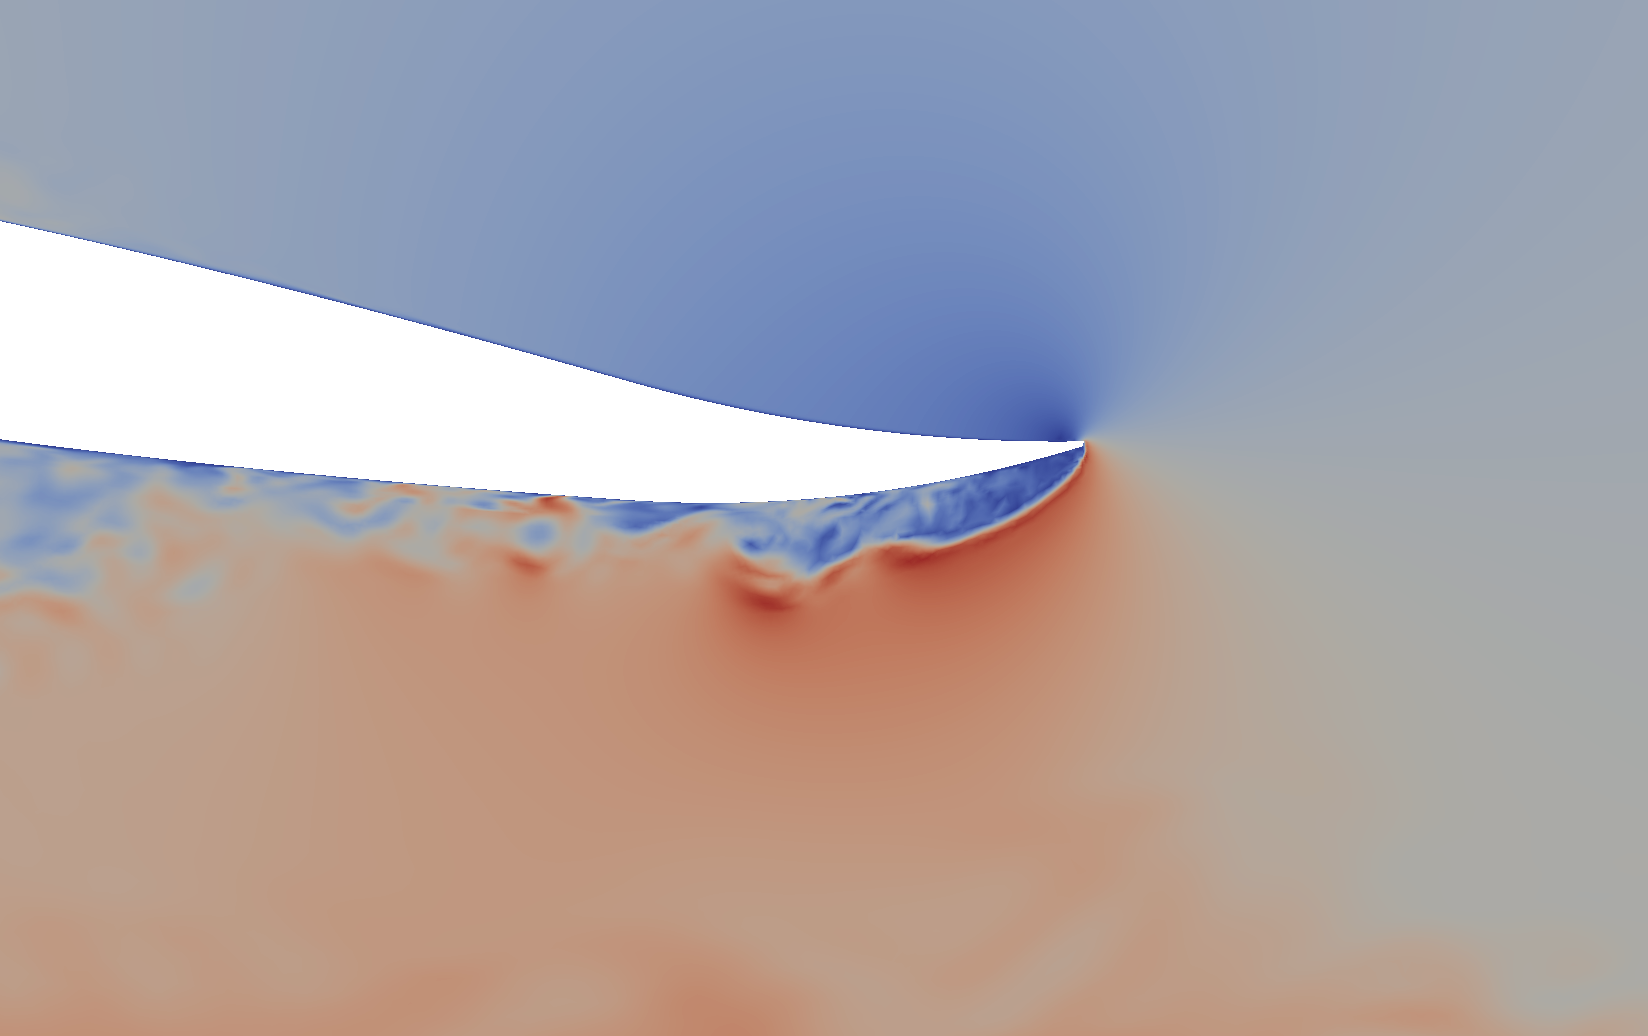
\includegraphics[width=1\textwidth]{figures/mu_1pt5/AC/ph_270_velocity_zoomed_airfoil_0_to_1pt5.png}
		\caption{actuated}
		\label{fig:mu_1pt5_AC_zoomed_velocity}
	\end{subfigure}
	\caption{Instantaneous velocity magnitude at $\psi$ = $270^\circ$ for the baseline (left column) and actuated (right column) cases at $\mu_{sect}$ = 1.5}
	\label{fig:mu_1pt5_zoomed_velocity}
\end{figure}

\begin{figure}[H]
	\centering
	
	\begin{subfigure}[b]{0.4\textwidth}
		\centering
		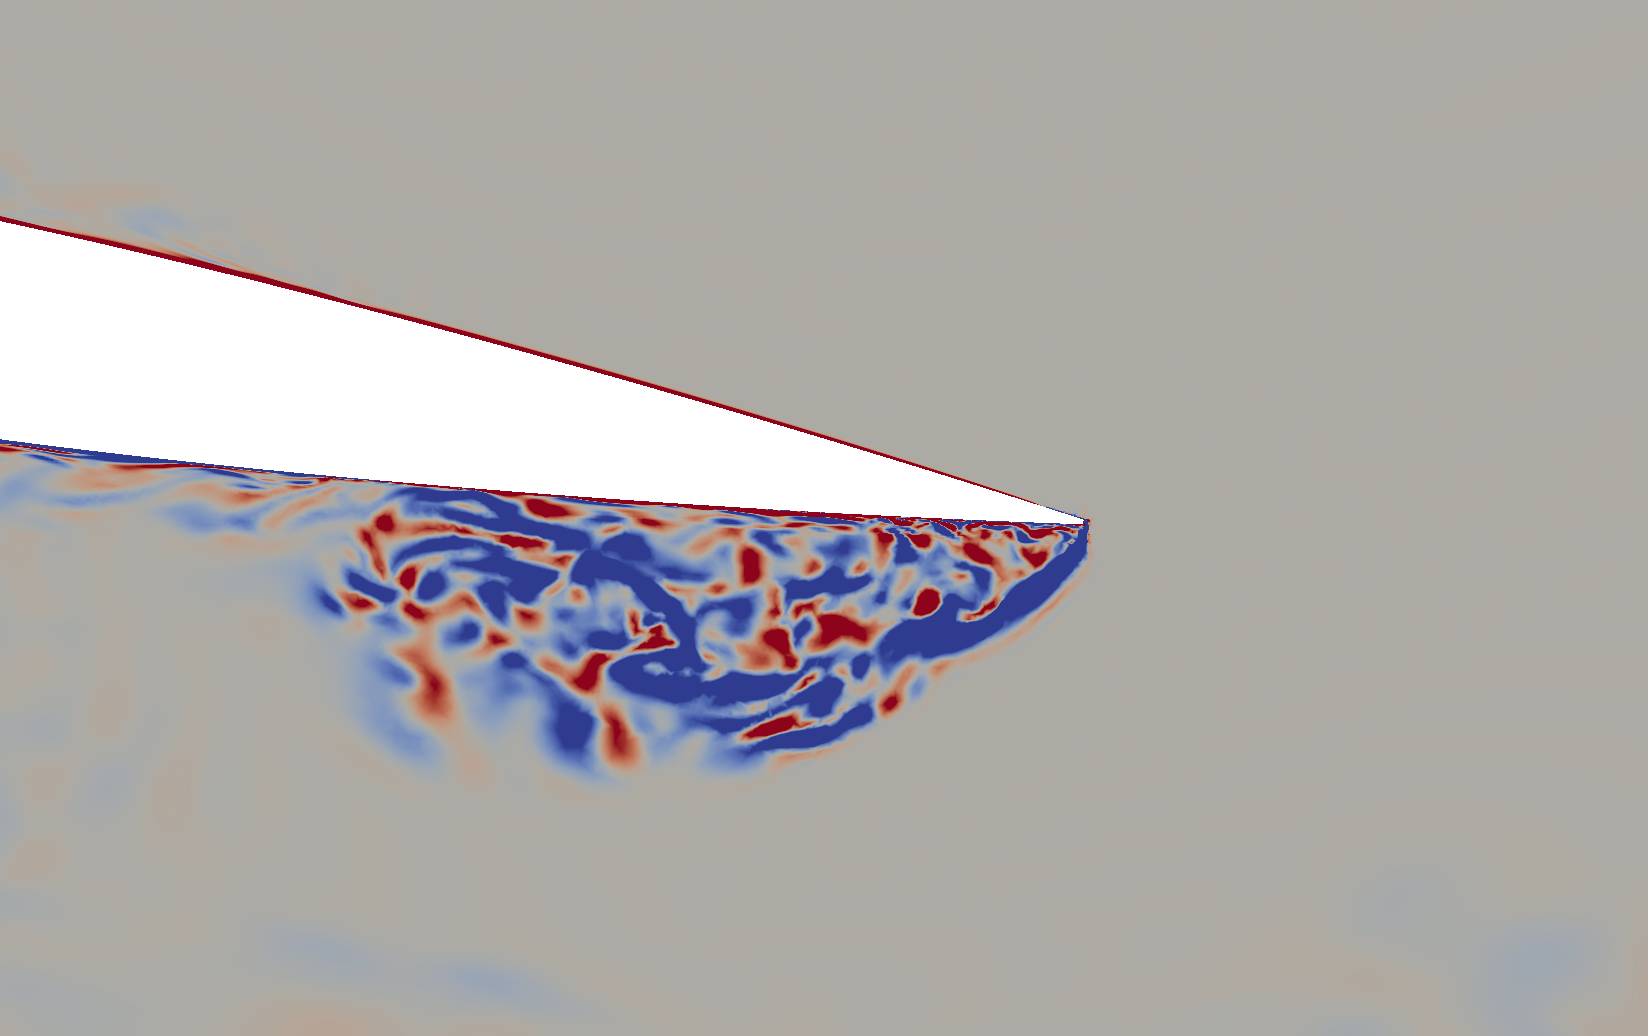
\includegraphics[width=1\textwidth]{figures/mu_1pt5/baseline/ph_270_vorticity_zoomed_airfoil.png}
		\caption{ baseline}
		\label{fig:mu_1pt5_baseline_zoomed_vorticity}
	\end{subfigure}
	\begin{subfigure}[b]{0.4\textwidth}
		\centering
		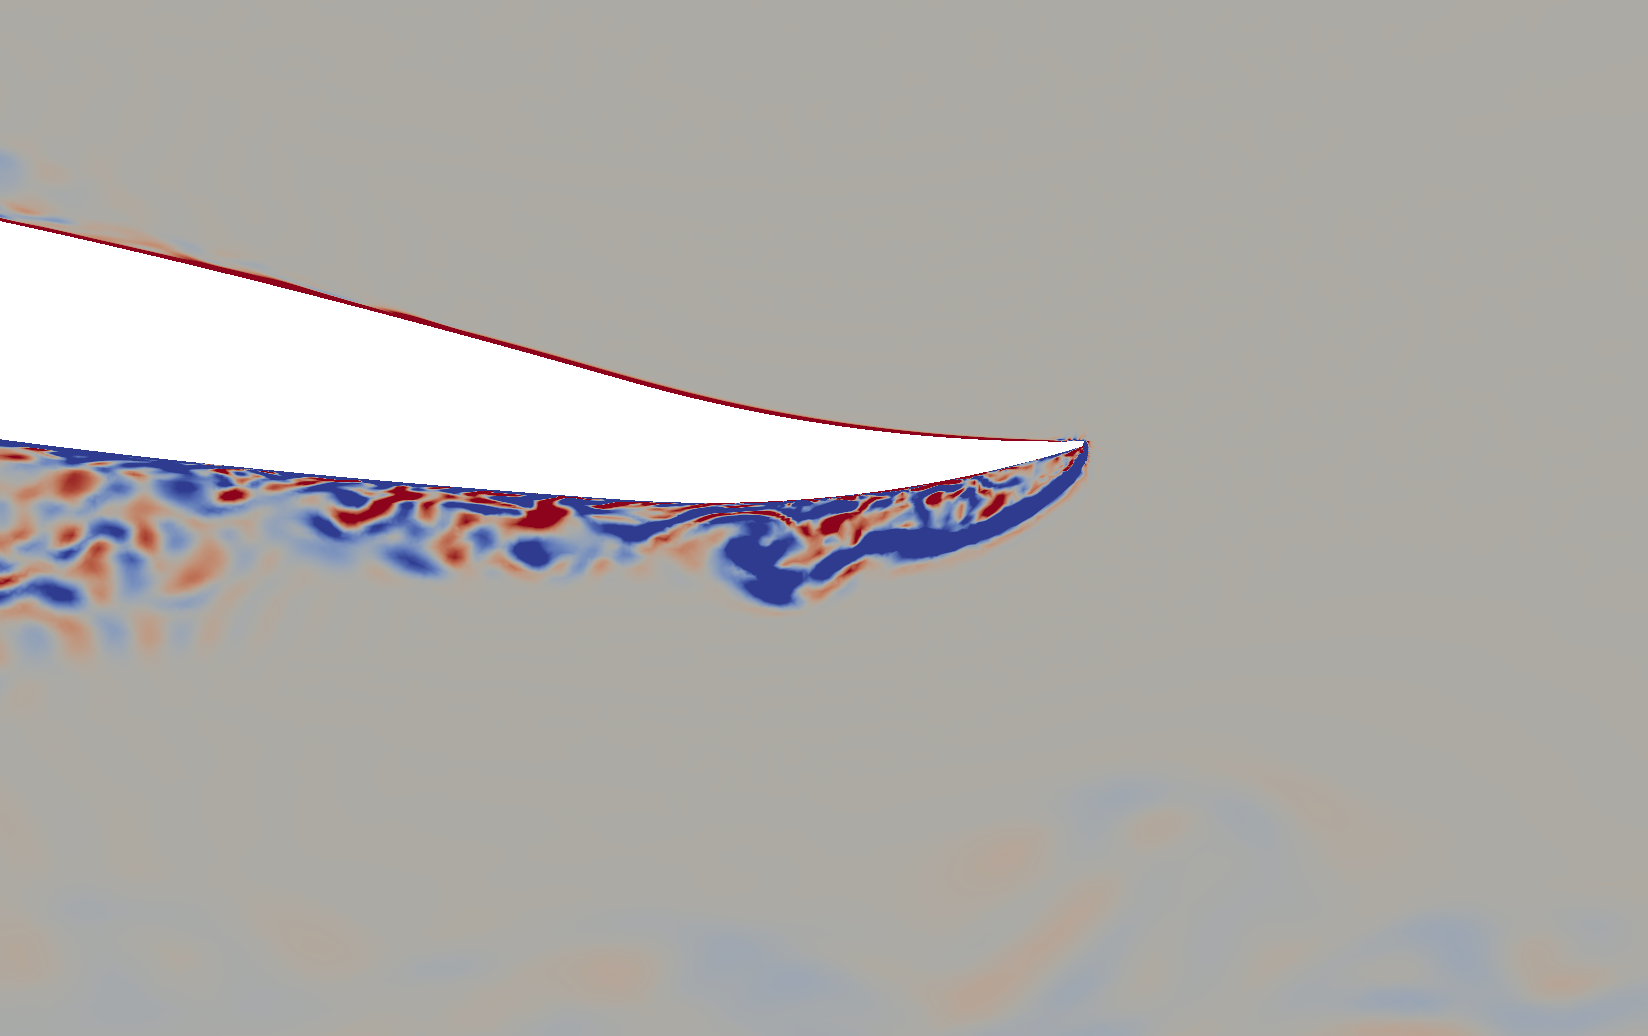
\includegraphics[width=1\textwidth]{figures/mu_1pt5/AC/ph_270_vorticity_zoomed_airfoil.png}
		\caption{actuated}
		\label{fig:mu_1pt5_AC_zoomed_vorticity}
	\end{subfigure}
	\caption{Instantaneous spanwise vorticity at $\psi$ = $270^\circ$ for the baseline (left column) and actuated (right column) cases at $\mu_{sect}$ = 1.5}
	\label{fig:mu_1pt5_zoomed_vorticity}
\end{figure}

\begin{figure}[H]
	\centering
	
	\begin{subfigure}[b]{0.4\textwidth}
		\centering
		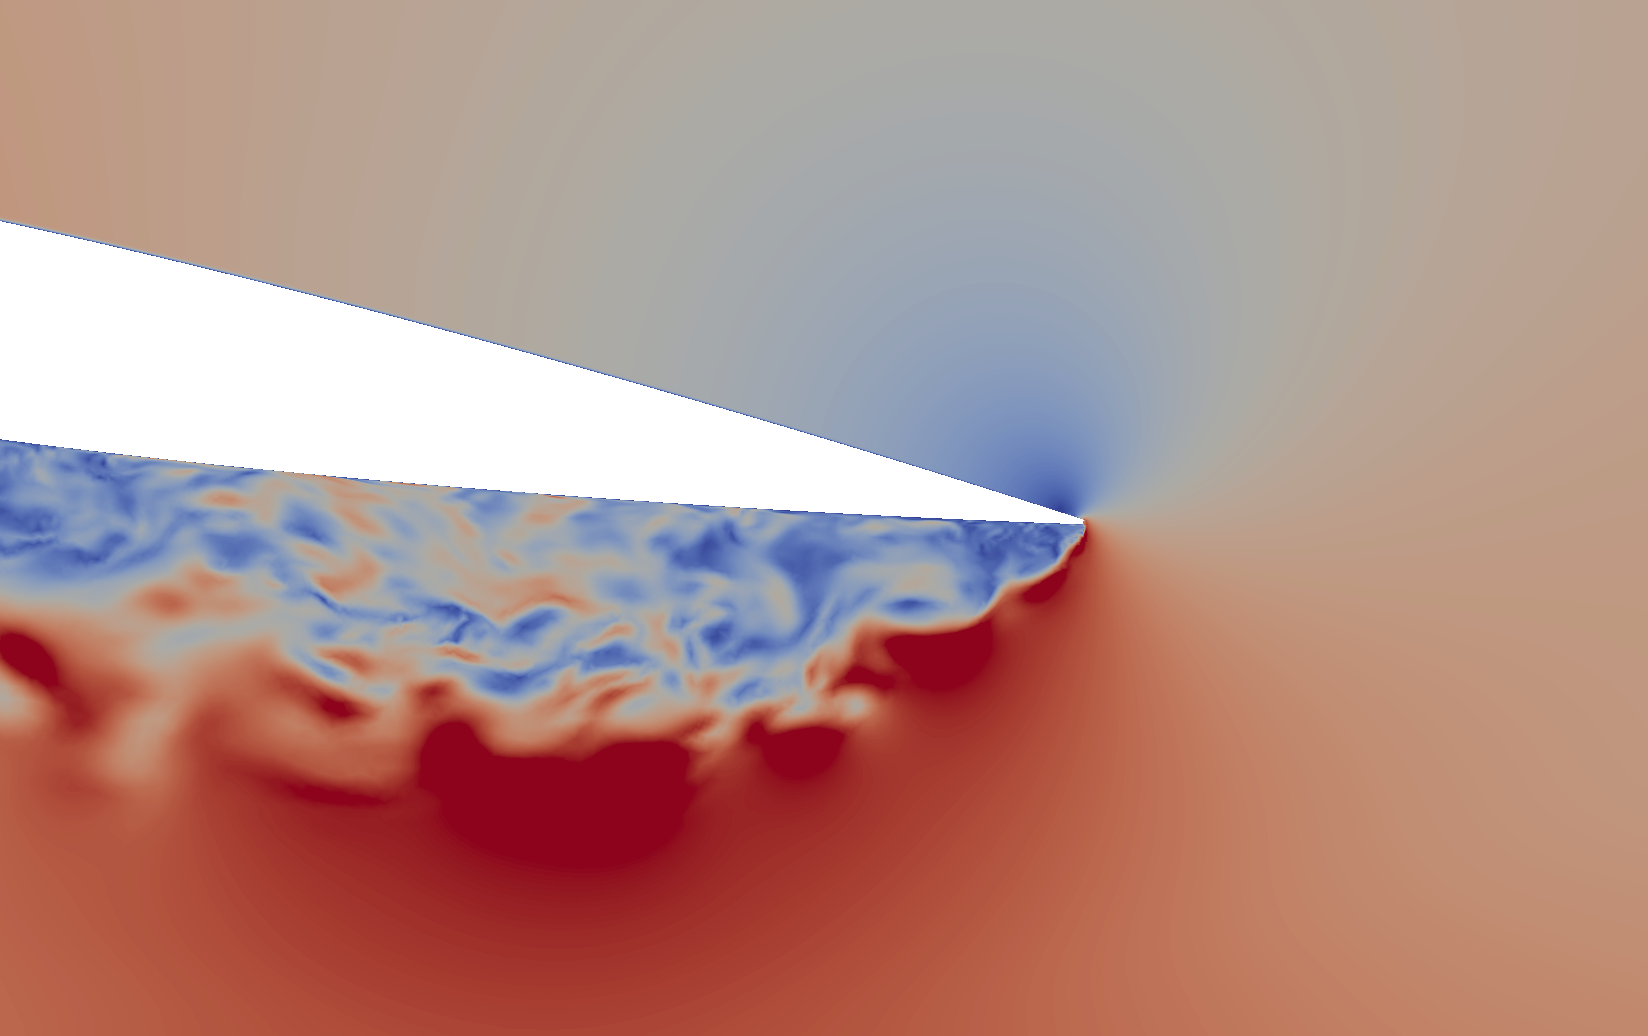
\includegraphics[width=1\textwidth]{figures/mu_2pt0/baseline/ph_270_velocity_zoomed_airfoil_0_to_1pt5.png}
		\caption{ baseline}
		\label{fig:mu_2pt0_baseline_zoomed_velocity}
	\end{subfigure}
	\begin{subfigure}[b]{0.4\textwidth}
		\centering
		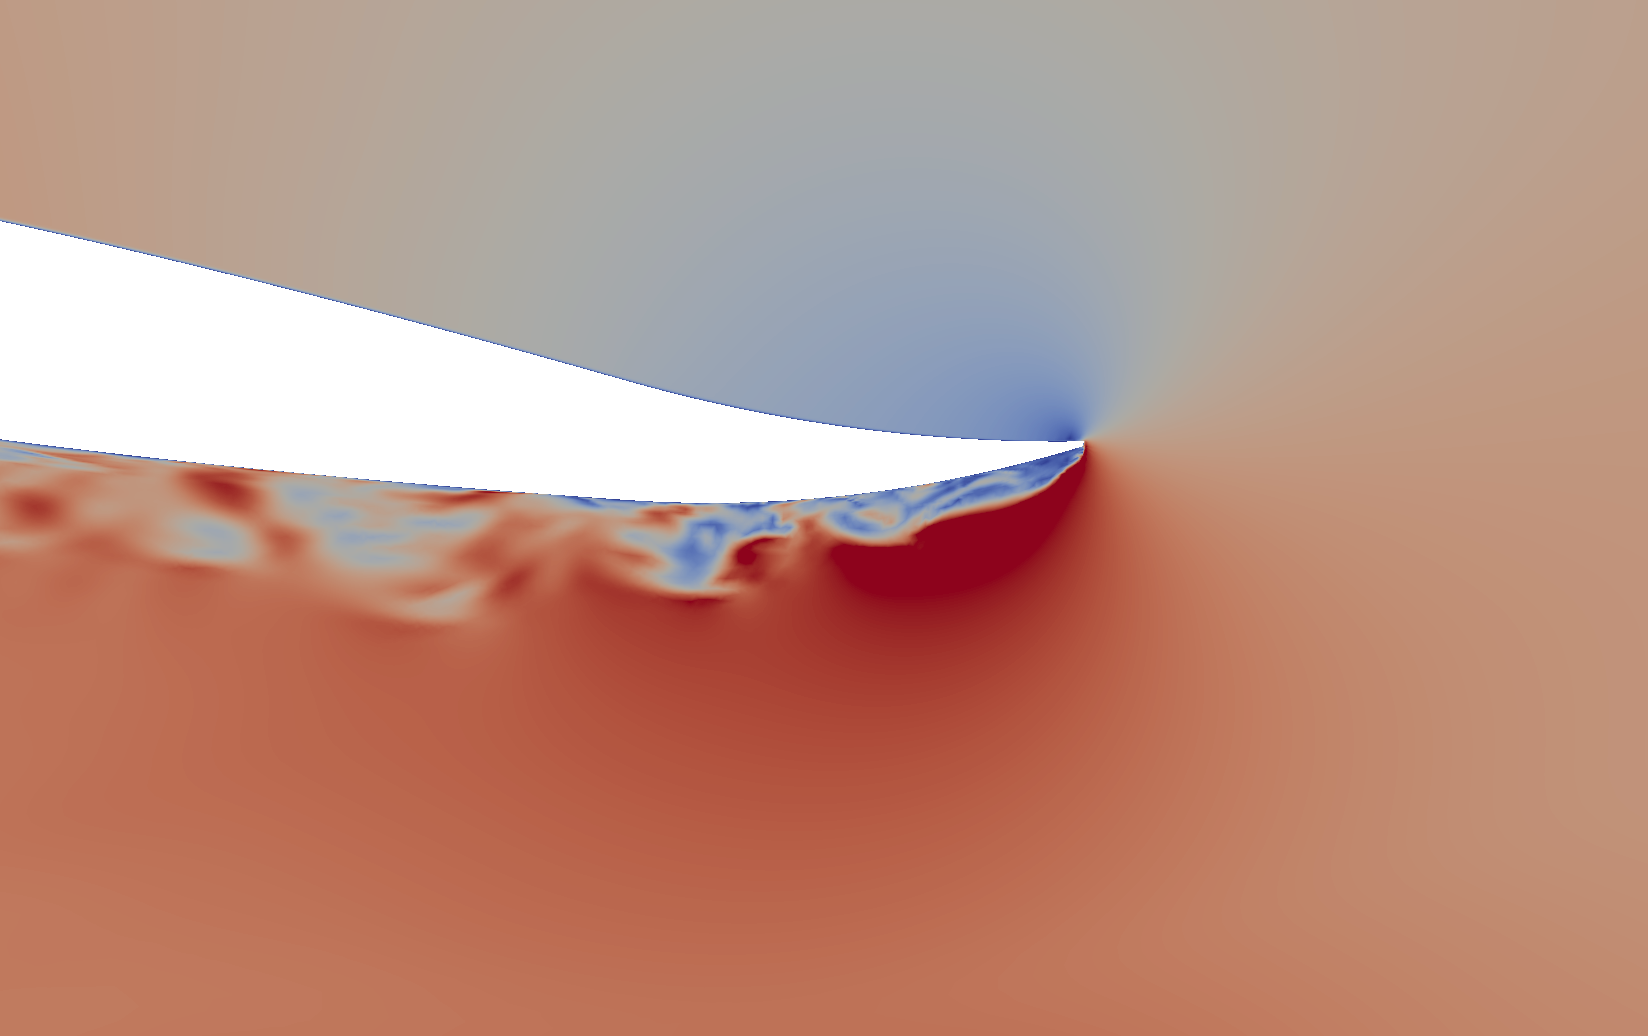
\includegraphics[width=1\textwidth]{figures/mu_2pt0/AC/ph_270_velocity_zoomed_airfoil_0_to_1pt5.png}
		\caption{actuated}
		\label{fig:mu_2pt0_AC_zoomed_velocity}
	\end{subfigure}
	\caption{Instantaneous velocity magnitude at $\psi$ = $270^\circ$ for the baseline (left column) and actuated (right column) cases at $\mu_{sect}$ = 2.0}
	\label{fig:mu_2pt0_zoomed_velocity}
\end{figure}

\begin{figure}[H]
	\centering
	
	\begin{subfigure}[b]{0.4\textwidth}
		\centering
		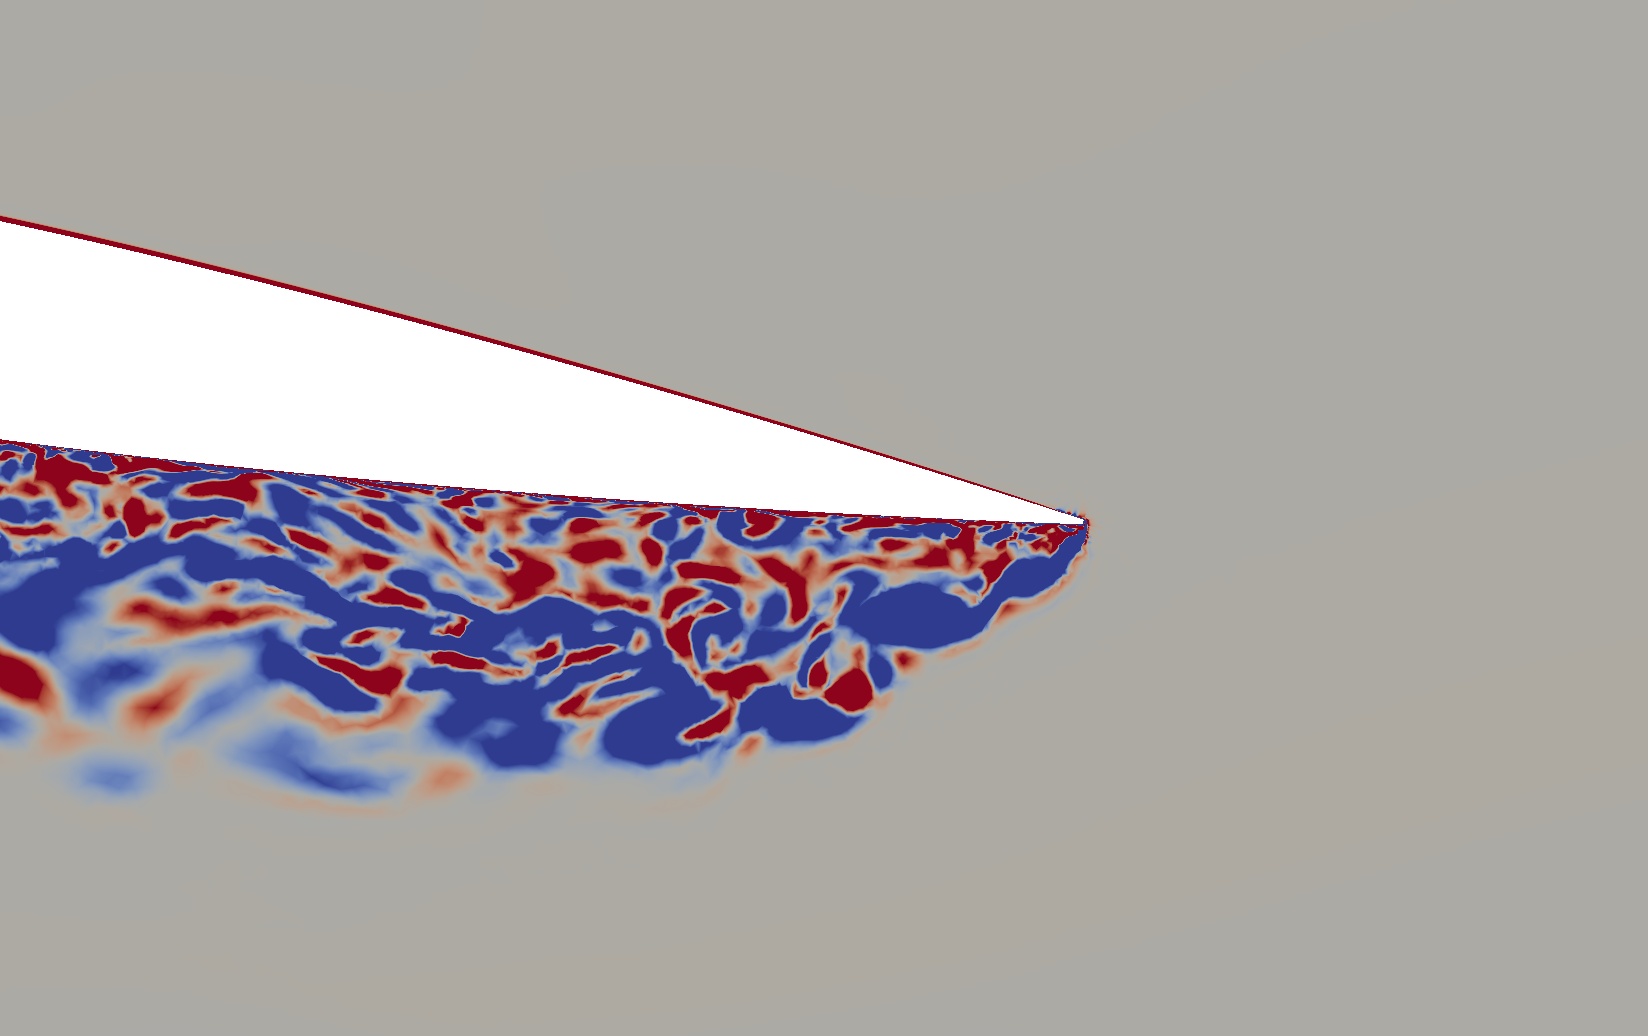
\includegraphics[width=1\textwidth]{figures/mu_2pt0/baseline/ph_270_vorticity_zoomed_airfoil.png}
		\caption{ baseline}
		\label{fig:mu_2pt0_baseline_zoomed_vorticity}
	\end{subfigure}
	\begin{subfigure}[b]{0.4\textwidth}
		\centering
		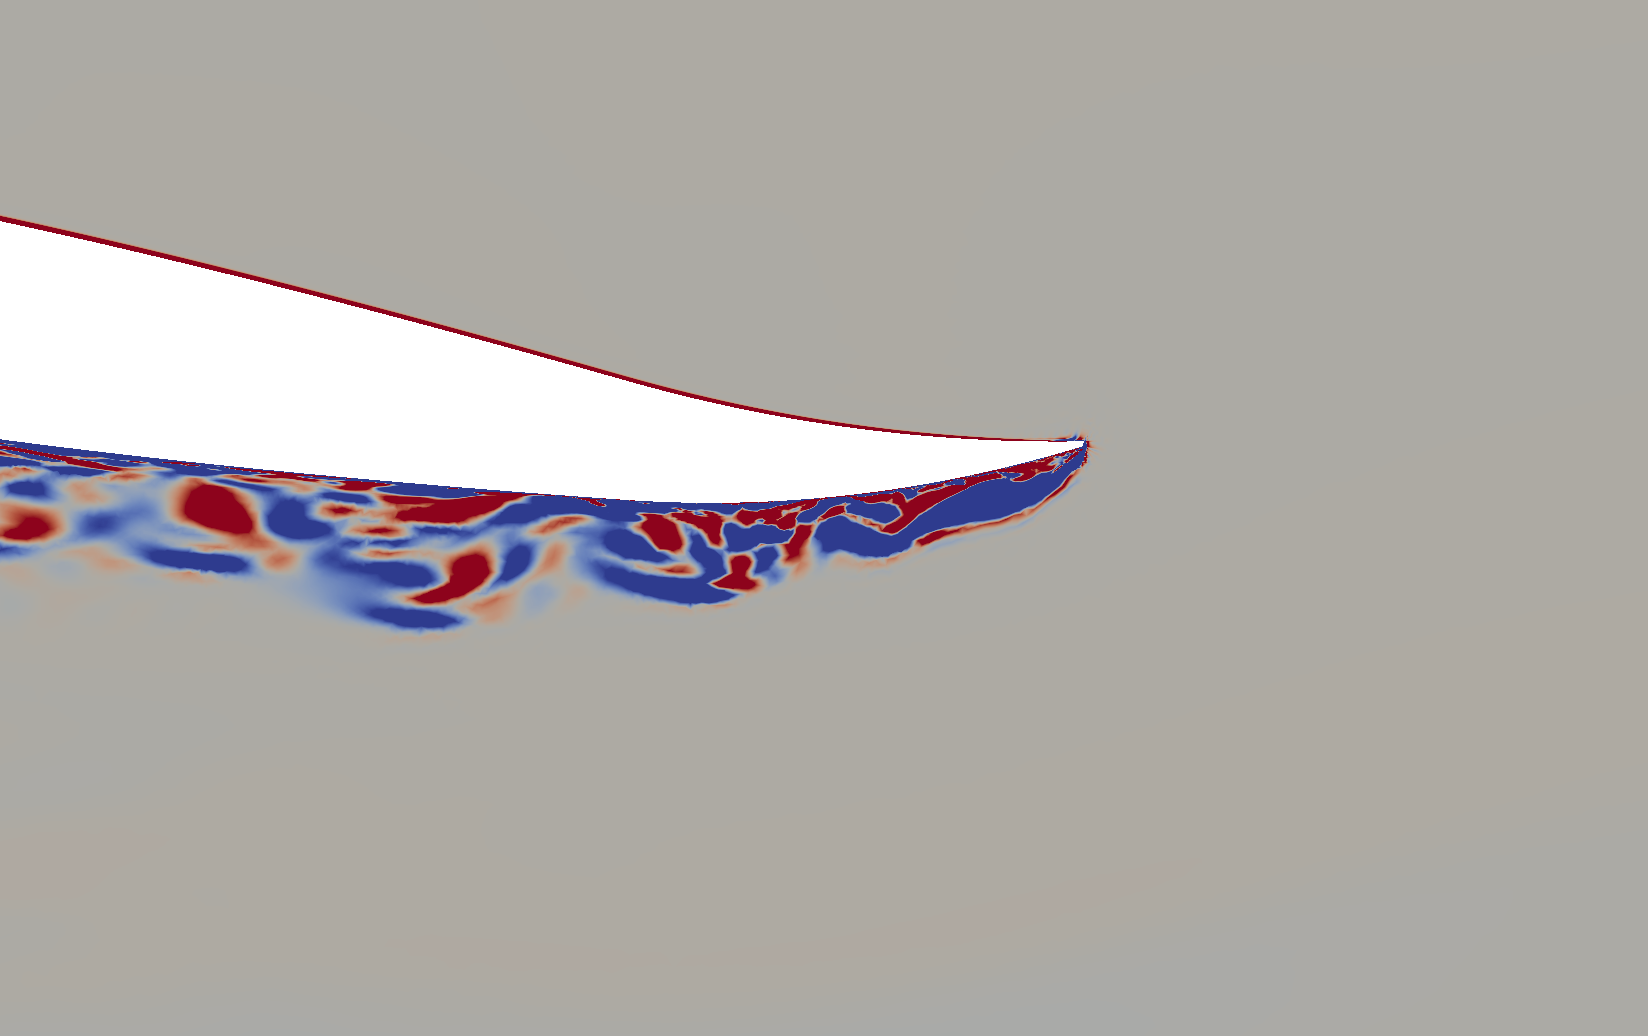
\includegraphics[width=1\textwidth]{figures/mu_2pt0/AC/ph_270_vorticity_zoomed_airfoil.png}
		\caption{actuated}
		\label{fig:mu_2pt0_AC_zoomed_vorticity}
	\end{subfigure}
	\caption{Instantaneous spanwise vorticity at $\psi$ = $270^\circ$ for the baseline (left column) and actuated (right column) cases at $\mu_{sect}$ = 2.0}
	\label{fig:mu_2pt0_zoomed_vorticity}
\end{figure}

%% mu_sect = 2.0
Figure \ref{fig:vortScreen_mu2pt0_SC1095} shows the instantaneous spanwise vorticity at sectional advance ratio of $\mu_{sect}=2.0$.
As before, 8 different phases over the retreating phase of the cycle are shown and the vorticity range is selected to be [-30,30]$ U_{sect} /C$. For this advance ratio, the airfoil enters the reverse flow region at $\psi=210^\circ$, and exits the reverse flow at $\psi=330^\circ$.
Reflex camber is activated at the phase of $\psi$=$200^\circ$ and reaches the full deflection at $\psi$=$205^\circ$.
After the airfoil exits the reverse flow, the reflexed airfoil starts returning to its undeflected position at $\psi$=$335^\circ$, and smoothly reaches its original shape at $\psi$=$340^\circ$.

As the airfoil trailing edge is deflected upwards for this actuated case with $\mu_{sect}=2.0$, a small vortex is formed near it, see Figure \ref{fig:mu_2pt0_AC_psi210}, which is similar to the actuated case with $\mu_{sect}=1.5$. Roll up of the boundary layer and LEV formation is seen for both baseline and actuated cases at $\psi$=$210^\circ$.
The flow separation near the trailing edge starts to form at an earlier phase of $\psi$=$225^\circ$, as compared to $\psi$=$240^\circ$ for the lower sectional advance ratio of $\mu_{sect}=1.5$.

In the subsequent phases after $\psi$=$225^\circ$ the size of the separated region increases for the baseline case till up to $\psi$=$285^\circ$. However, the separation bubble is larger in the baseline case with $\mu_{sect}=2.0$ as compared to that with $\mu_{sect}=1.5$.
For the actuated case, the separated region is relatively small (see Figures \ref{fig:mu_2pt0_baseline_psi270} and \ref{fig:mu_2pt0_AC_psi270}) and its size remains fairly constant between phases $\psi$=$255^\circ$ and $285^\circ$ (see Figures \ref{fig:mu_2pt0_AC_psi255}, \ref{fig:mu_2pt0_AC_psi270} and \ref{fig:mu_2pt0_AC_psi285}).
As before, overall a significant reduction is observed in the size/extent as well as unsteadiness of the separation bubble near the trailing edge during the reverse flow region due to active reflex camber.

After $\psi$=$285^\circ$, the trailing-edge flow separation begins to wash away from the airfoil for both baseline and actuated cases, see Figures \ref{fig:mu_2pt0_baseline_psi315} and \ref{fig:mu_2pt0_AC_psi315}. 
For the actuated case at $\psi$=$345^\circ$, the reflexed trailing edge is at its undeflected position.
As the trailing edge is deflected down to its original position, this results in the formation of a small vortex as seen in Figure \ref{fig:mu_2pt0_AC_psi345}.

\begin{figure}[H]
	\centering
	
	\begin{subfigure}[b]{0.4\textwidth}
		\centering
		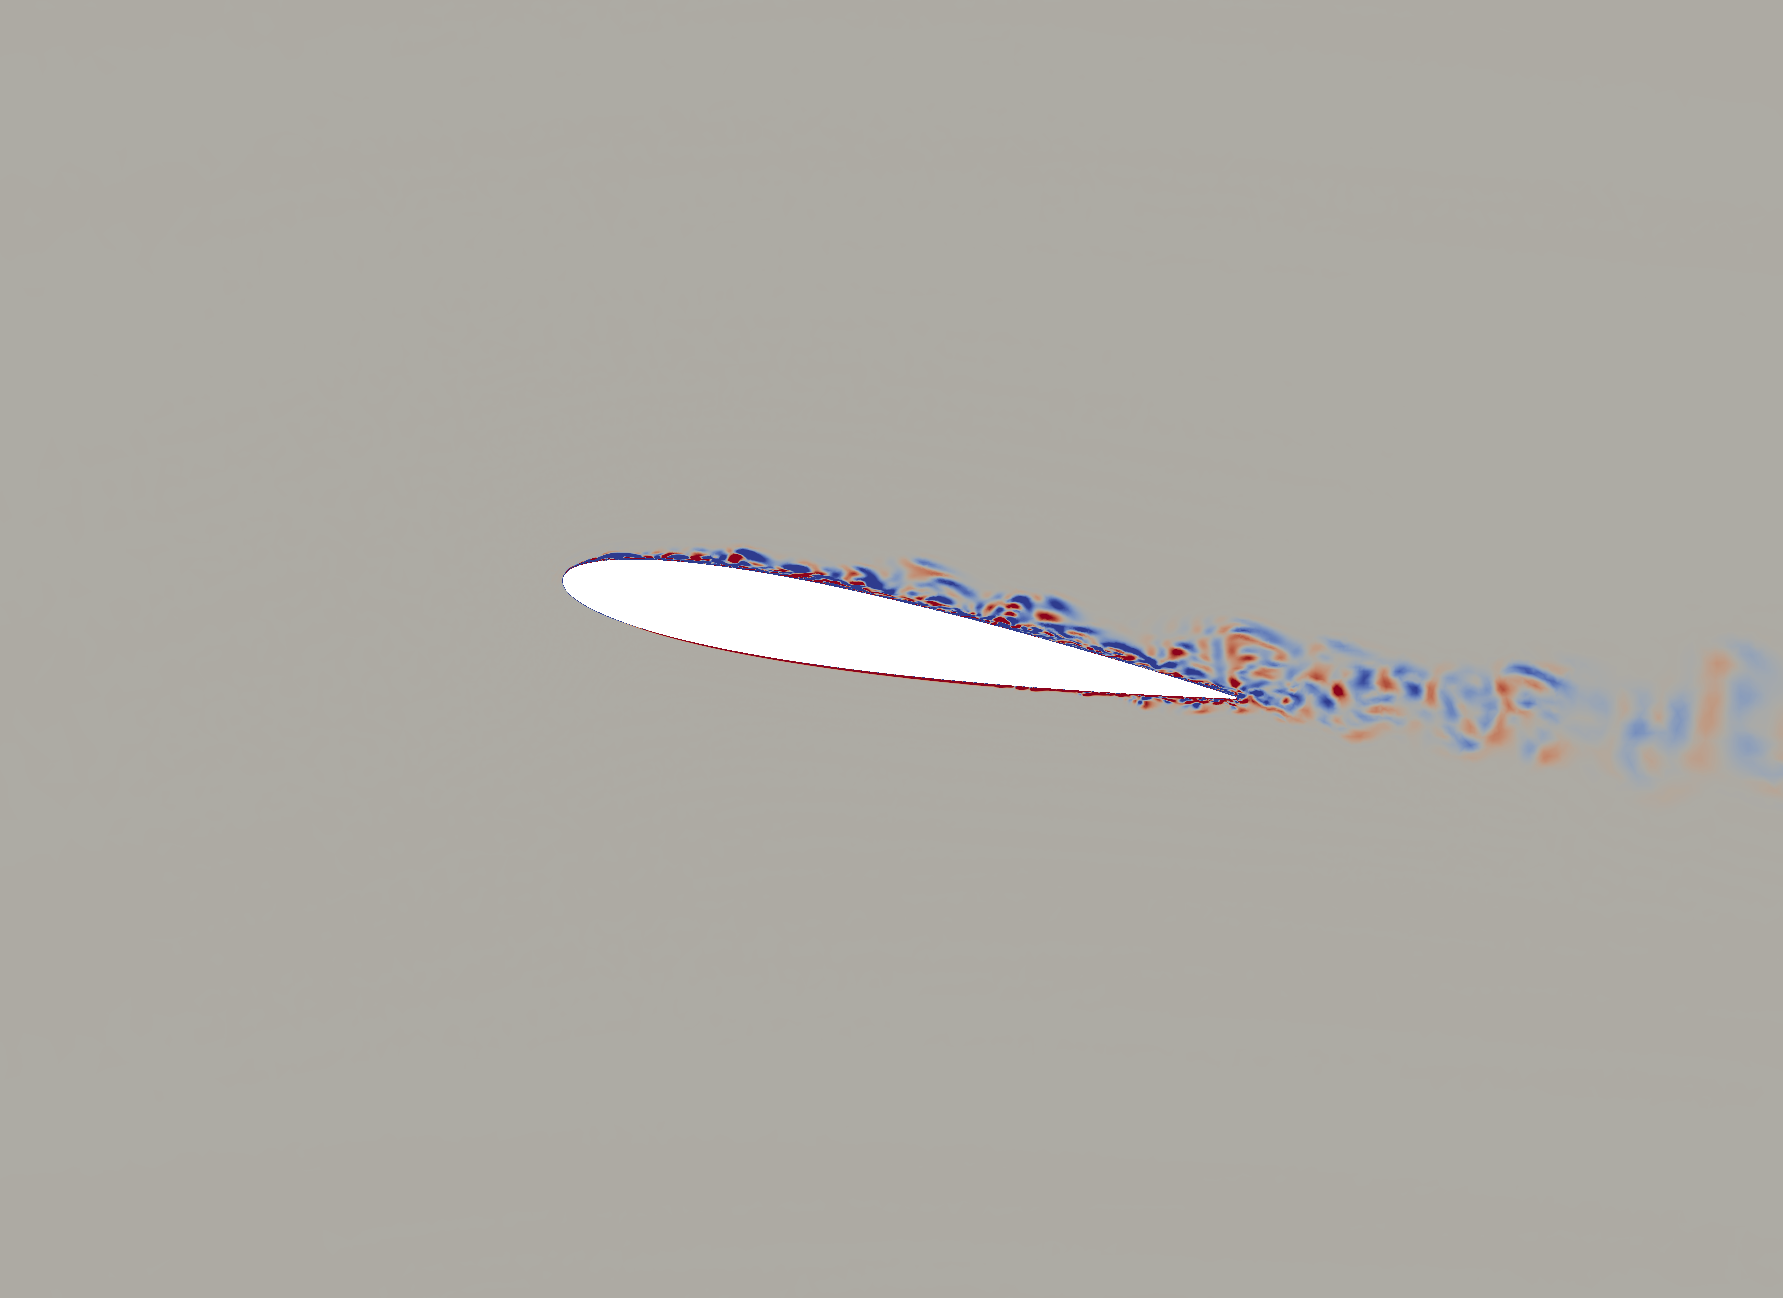
\includegraphics[width=1\textwidth]{figures/mu_2pt0/vorticity/baseline/phase_195.png}
		\caption{ $\psi$ = $195^\circ$, $\tilde{t}=0.542$}
		\label{fig:mu_2pt0_baseline_psi195}
	\end{subfigure}
	\begin{subfigure}[b]{0.4\textwidth}
		\centering
		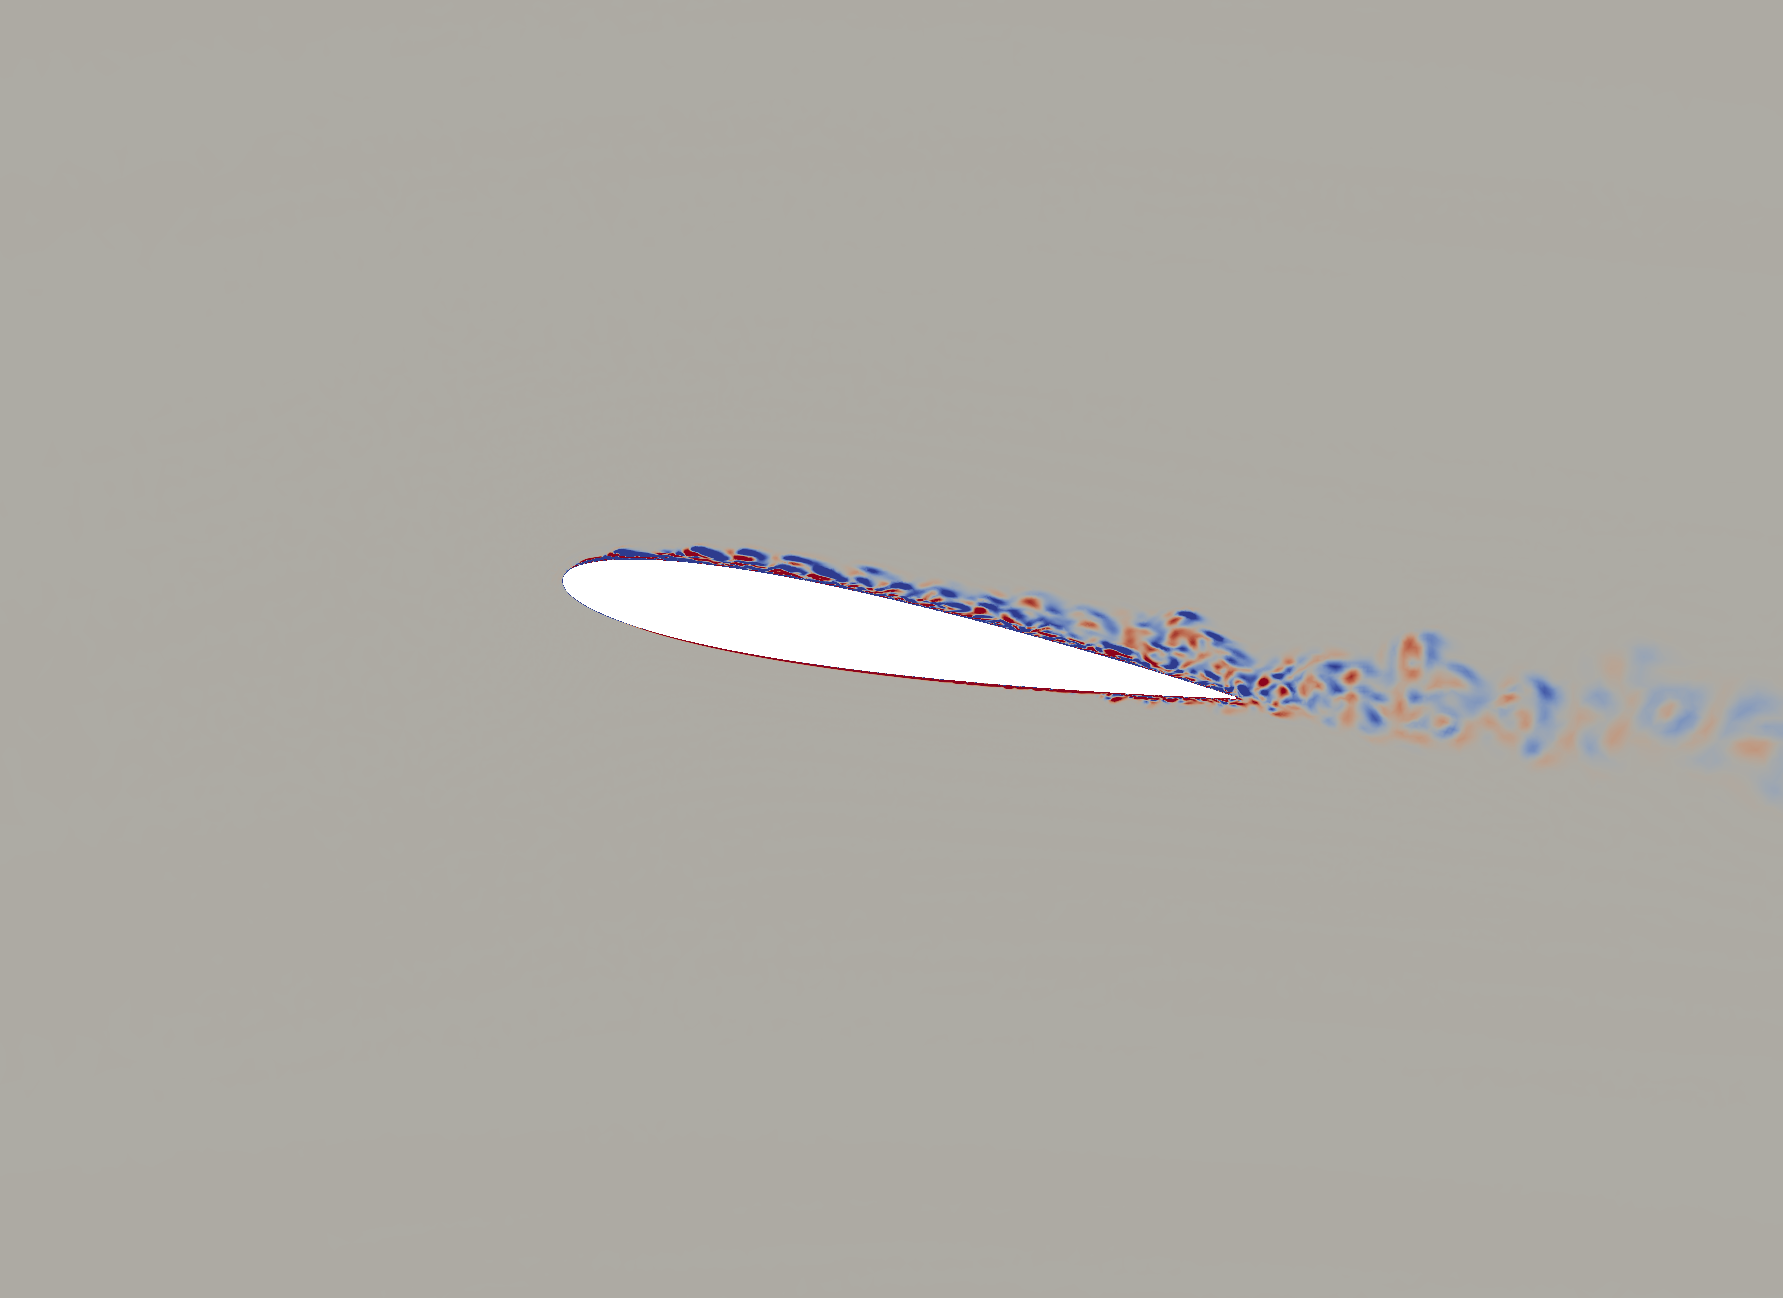
\includegraphics[width=1\textwidth]{figures/mu_2pt0/vorticity/AC/phase_195.png}
		\caption{ $\psi$ = $195^\circ$, $\tilde{t}=0.542$}
		\label{fig:mu_2pt0_AC_psi195}
	\end{subfigure}
	
	\begin{subfigure}[b]{0.4\textwidth}
		\centering
		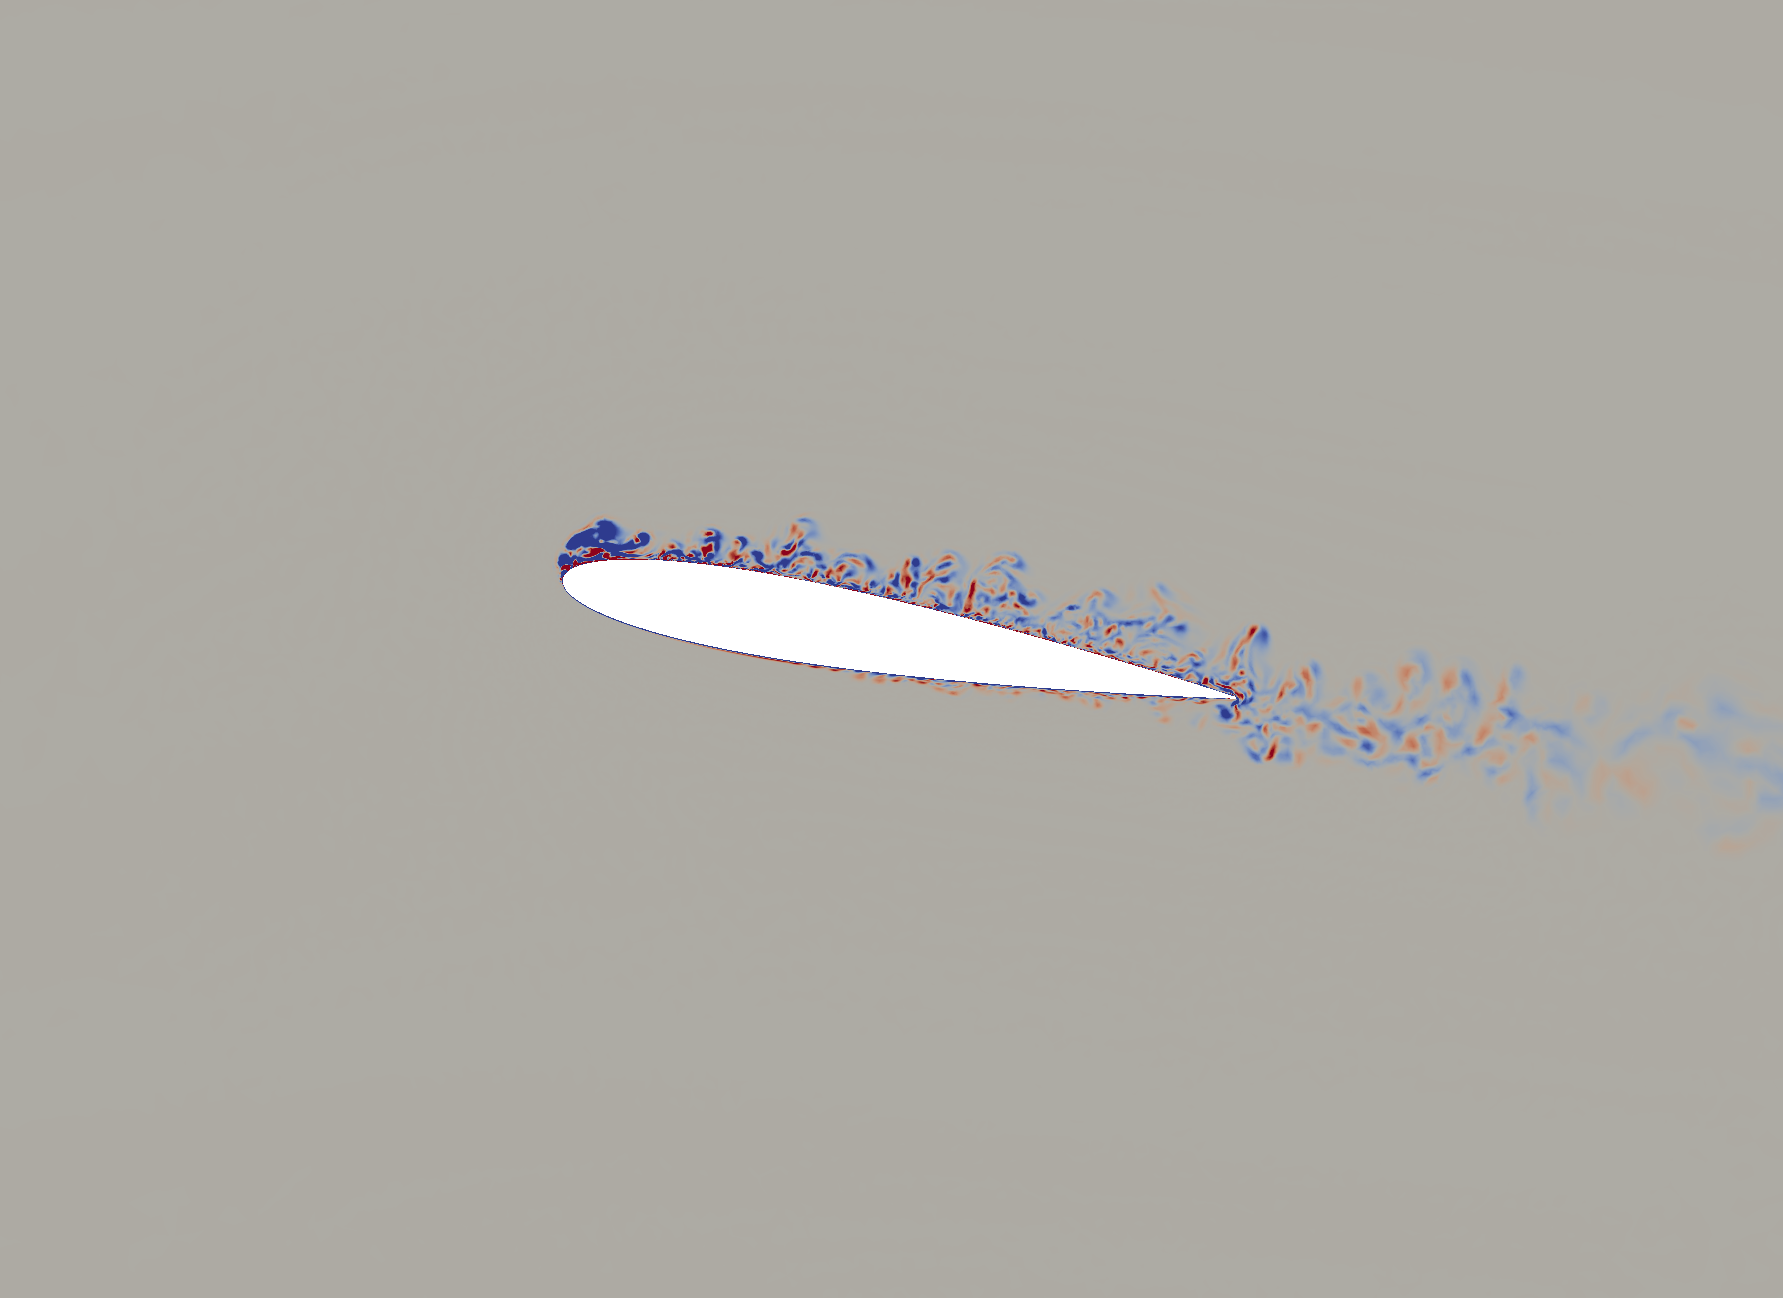
\includegraphics[width=1\textwidth]{figures/mu_2pt0/vorticity/baseline/phase_210.png}
		\caption{ $\psi$ = $210^\circ$, $\tilde{t}=0.542$}
		\label{fig:mu_2pt0_baseline_psi210}
	\end{subfigure}
	\begin{subfigure}[b]{0.4\textwidth}
		\centering
		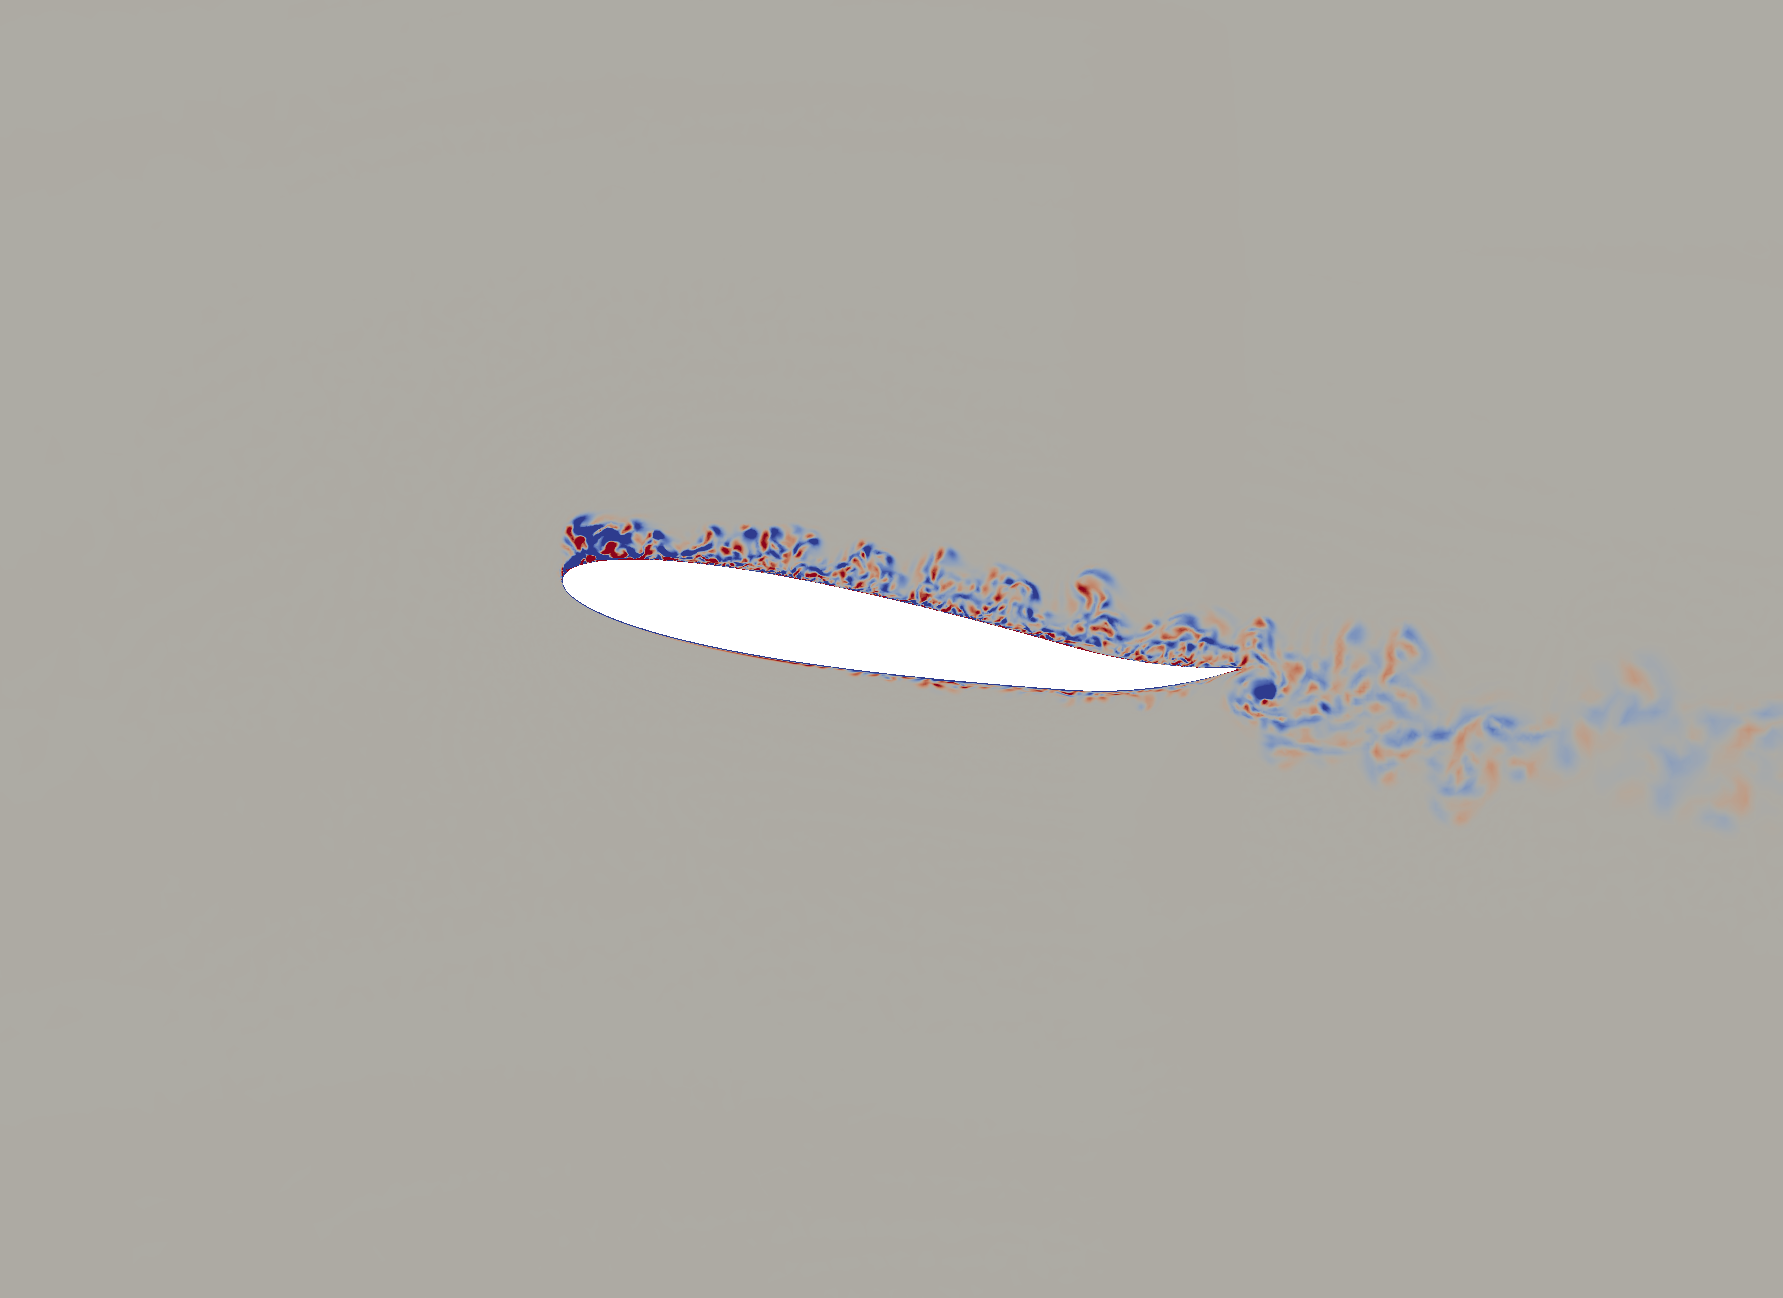
\includegraphics[width=1\textwidth]{figures/mu_2pt0/vorticity/AC/phase_210.png}
		\caption{ $\psi$ = $210^\circ$, $\tilde{t}=0.542$}
		\label{fig:mu_2pt0_AC_psi210}
	\end{subfigure}
	
	\begin{subfigure}[b]{0.4\textwidth}
		\centering
		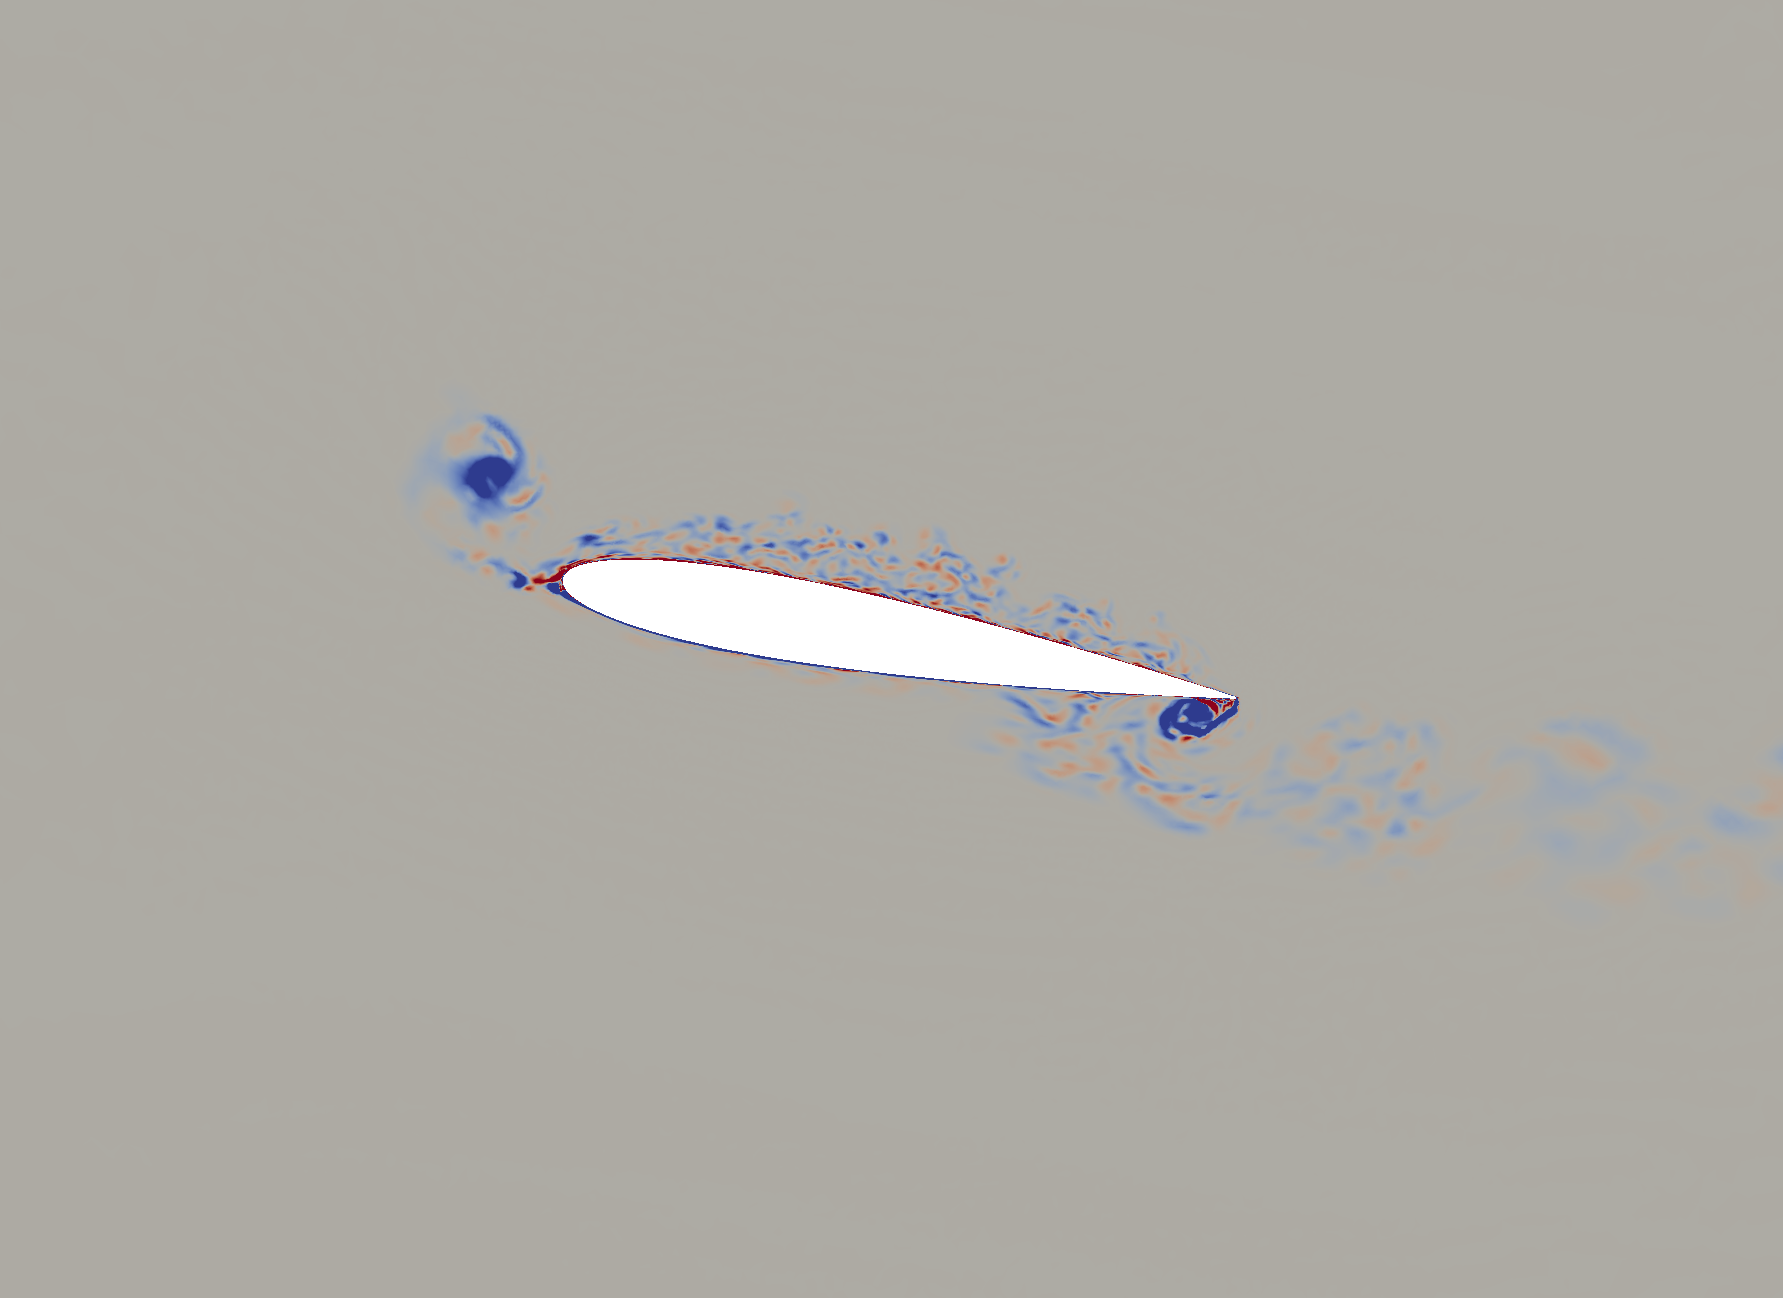
\includegraphics[width=1\textwidth]{figures/mu_2pt0/vorticity/baseline/phase_225.png}
		\caption{ $\psi$ = $225^\circ$, $\tilde{t}=0.625$}
		\label{fig:mu_2pt0_baseline_psi225}
	\end{subfigure}
	\begin{subfigure}[b]{0.4\textwidth}
		\centering
		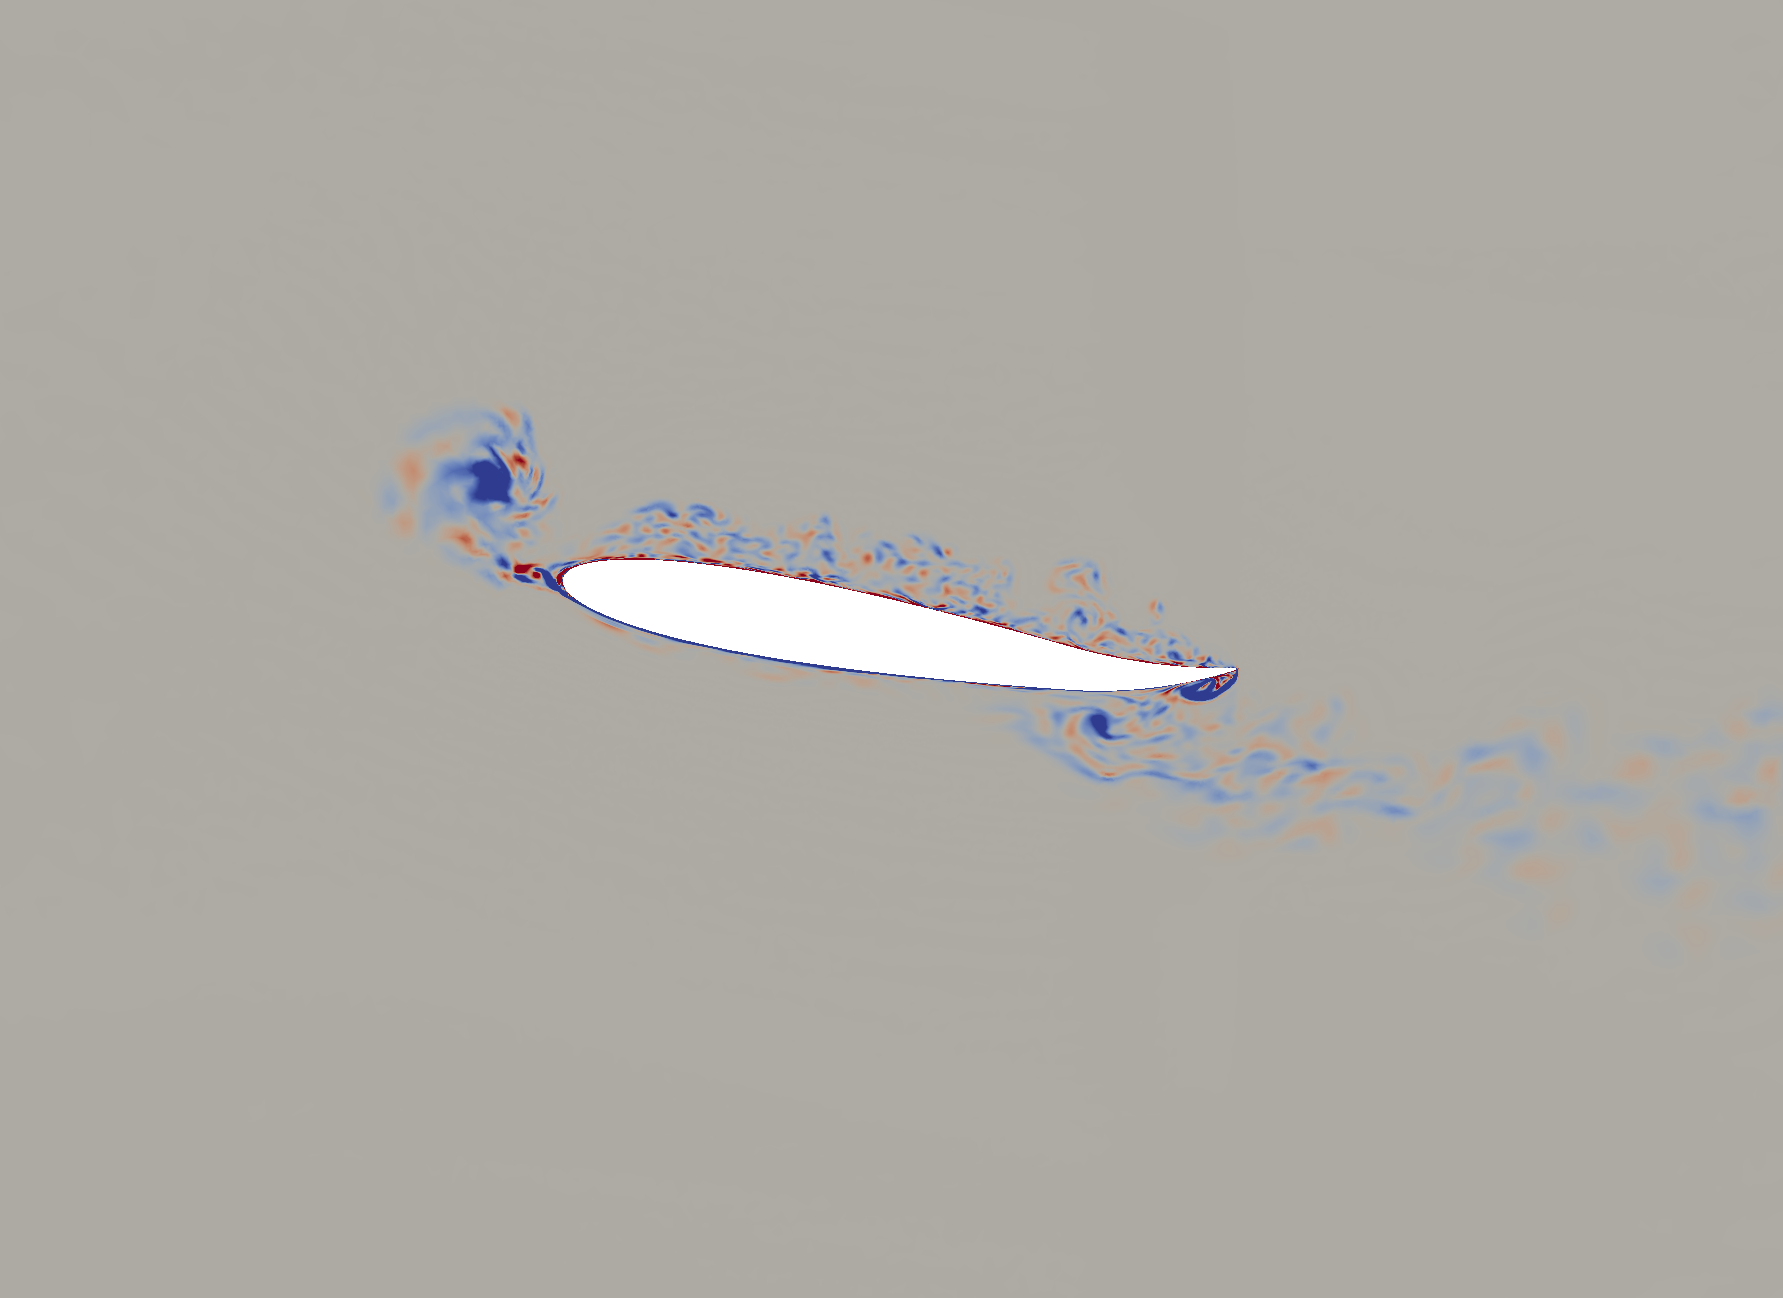
\includegraphics[width=1\textwidth]{figures/mu_2pt0/vorticity/AC/phase_225.png}
		\caption{ $\psi$ = $225^\circ$,  $\tilde{t}=0.625$}
		\label{fig:mu_2pt0_AC_psi225}
	\end{subfigure}
	
	
	%\begin{subfigure}[b]{0.4\textwidth}
	%	\centering
	%	 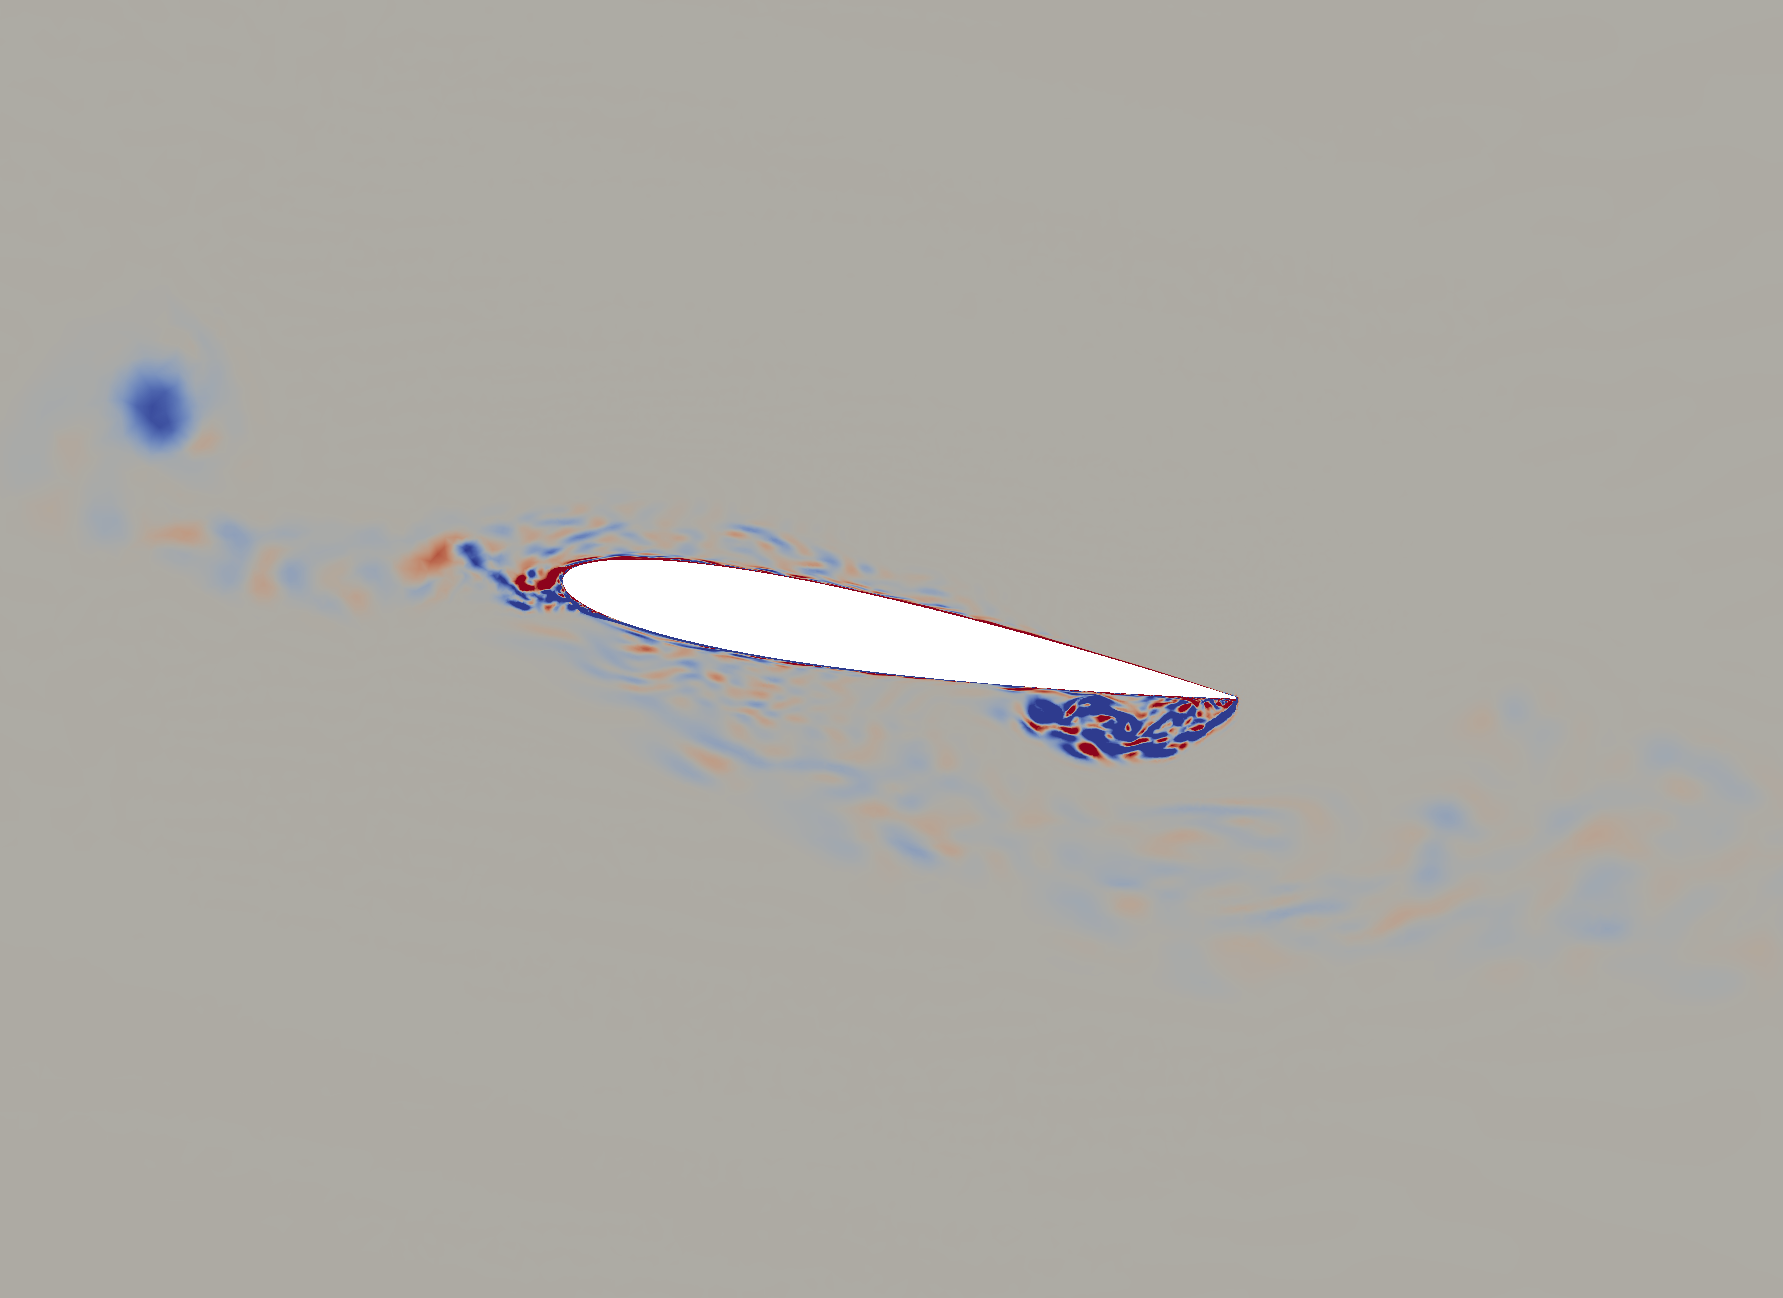
\includegraphics[width=1\textwidth]{figures/mu_2pt0/vorticity/baseline/phase_240.png}
	%	\caption{ $\psi$ = $240^\circ$, $\tilde{t}=0.667$}
	%	\label{fig:mu_2pt0_baseline_psi240}
	%\end{subfigure}
	%\begin{subfigure}[b]{0.4\textwidth}
	%	\centering
	%	 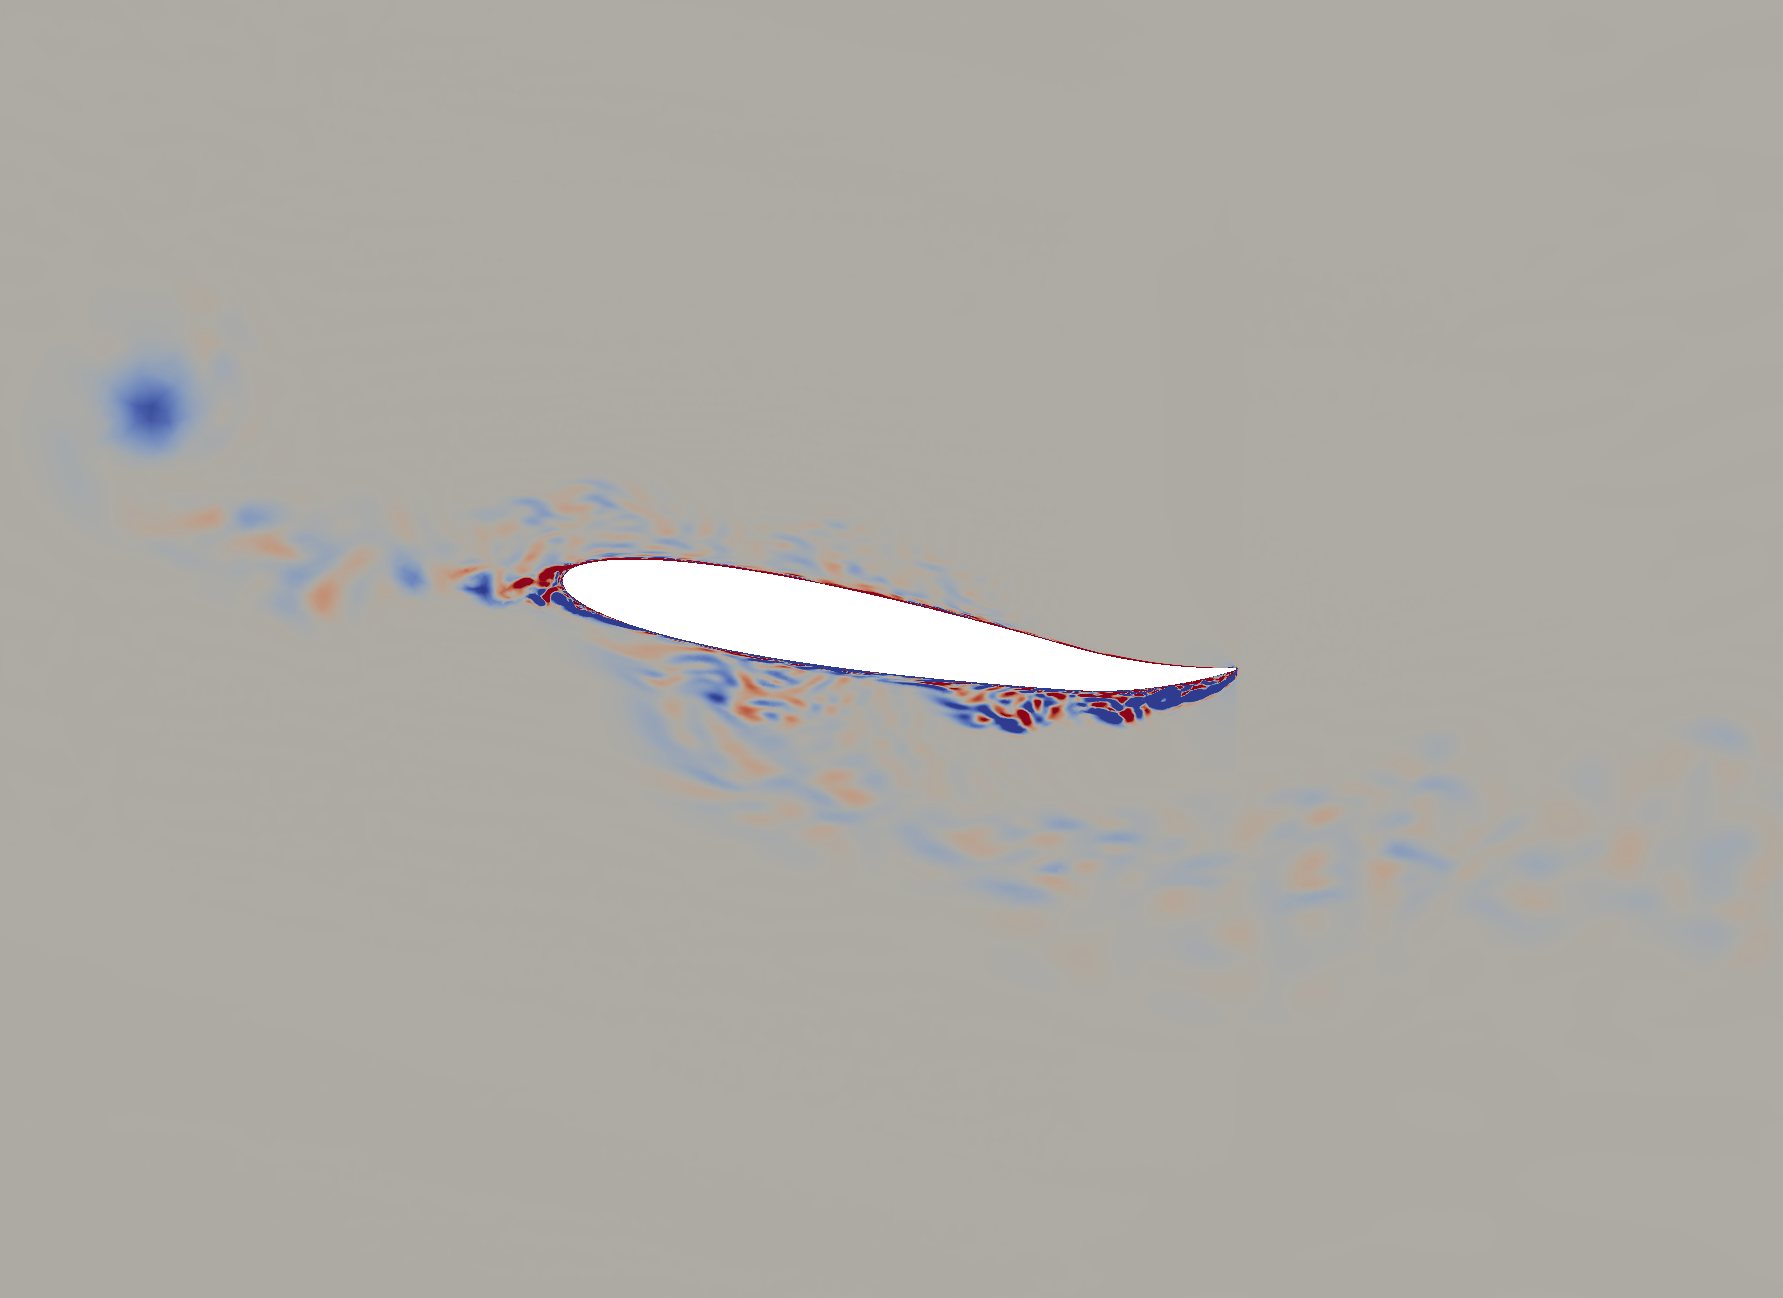
\includegraphics[width=1\textwidth]{figures/mu_2pt0/vorticity/AC/phase_240.png}
	%	\caption{ $\psi$ = $240^\circ$, $\tilde{t}=0.667$}
	%	\label{fig:mu_2pt0_AC_psi240}
	%\end{subfigure}
	
	\begin{subfigure}[b]{0.4\textwidth}
		\centering
		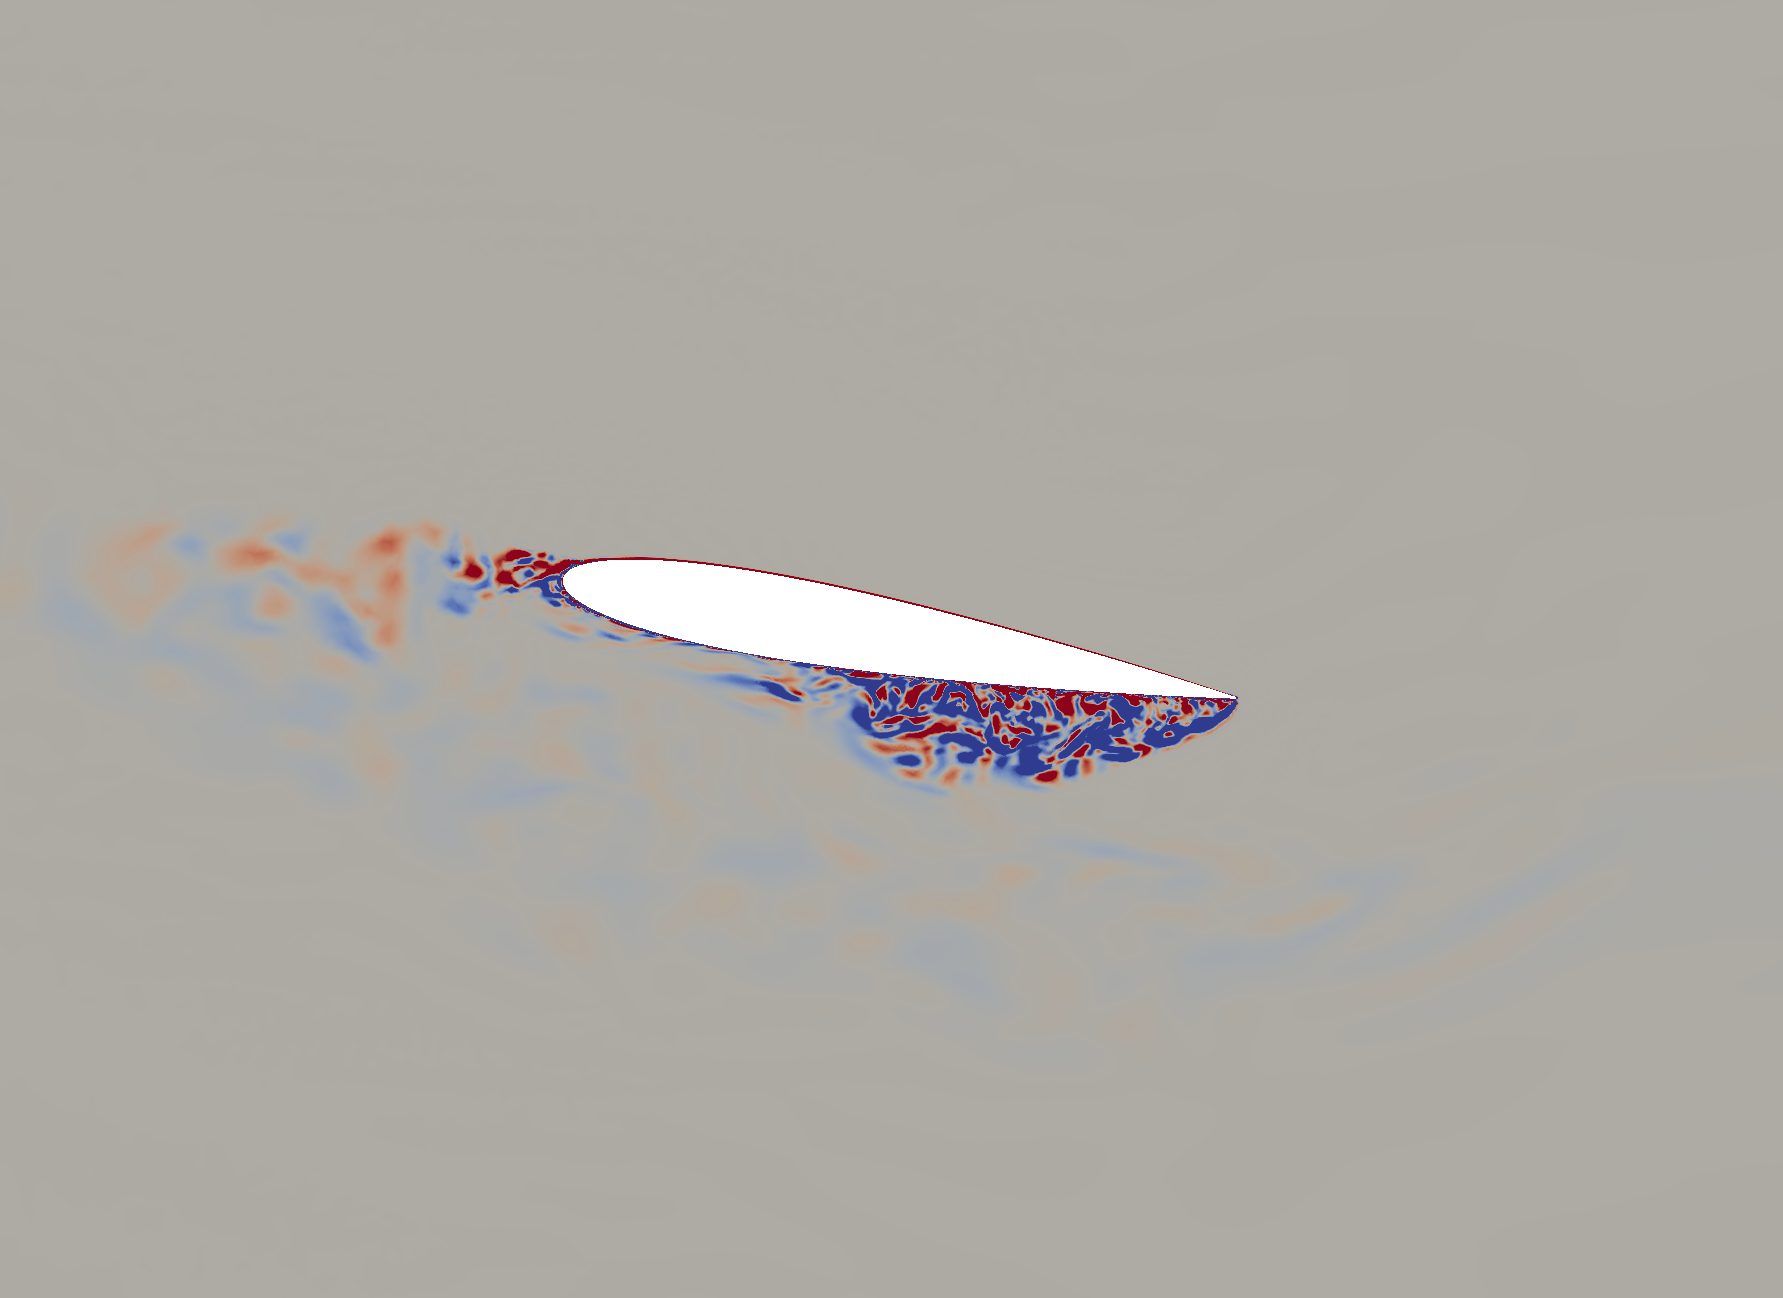
\includegraphics[width=1\textwidth]{figures/mu_2pt0/vorticity/baseline/phase_255.png}
		\caption{ $\psi$ = $255^\circ$, $\tilde{t}=0.708$}
		\label{fig:mu_2pt0_baseline_psi255}
	\end{subfigure}
	\begin{subfigure}[b]{0.4\textwidth}
		\centering
		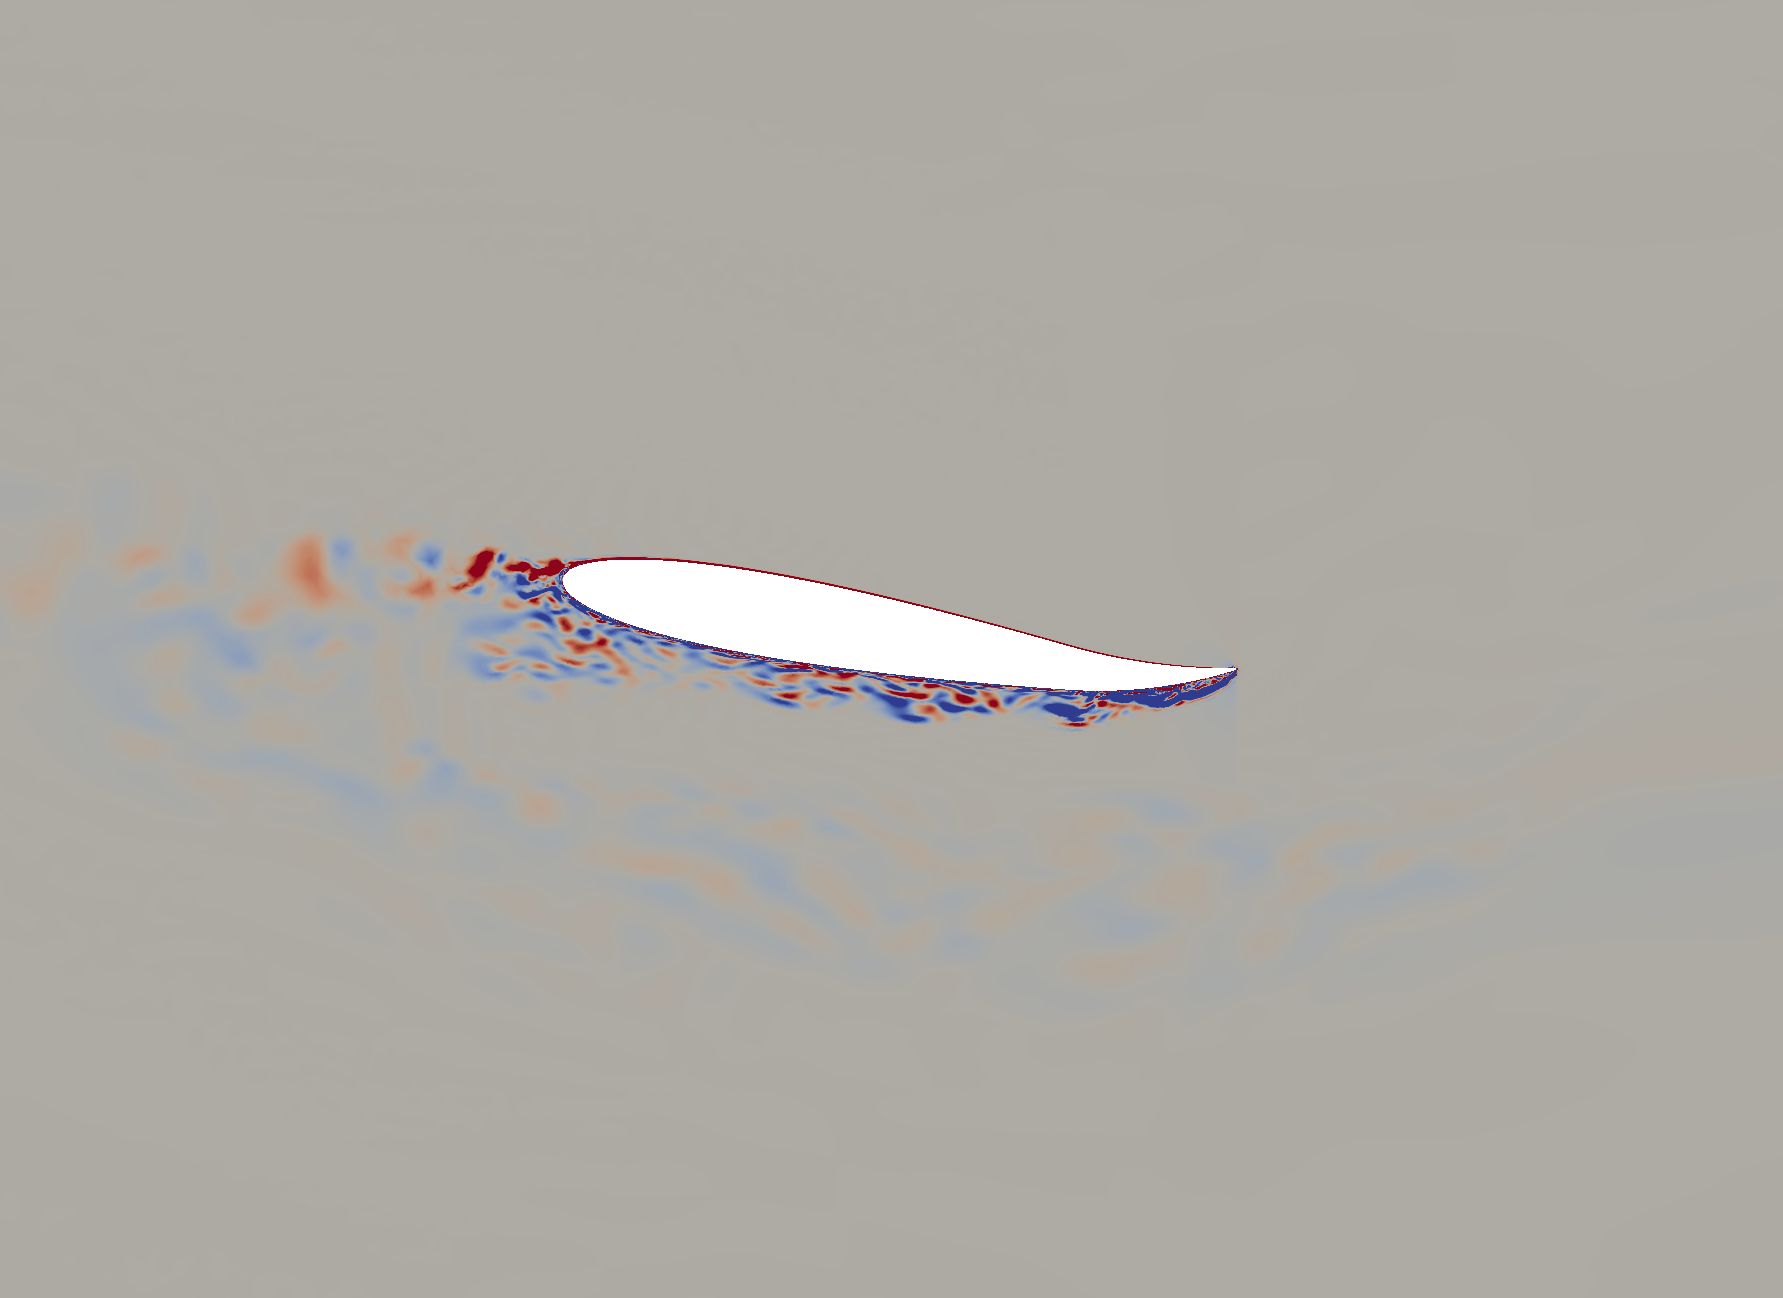
\includegraphics[width=1\textwidth]{figures/mu_2pt0/vorticity/AC/phase_255.png}
		\caption{ $\psi$ = $255^\circ$, $\tilde{t}=0.708$}
		\label{fig:mu_2pt0_AC_psi255}
	\end{subfigure}
	
	
	\caption{Instantaneous spanwise vorticity at 8 different phases for the baseline (left column) and actuated (right column) cases at $\mu_{sect}$ = 2.0}
	%\label{fig:vortScreen_mu2pt0}
\end{figure}

\begin{figure}[H]\ContinuedFloat
	\centering
	
	\begin{subfigure}[b]{0.4\textwidth}
		\centering
		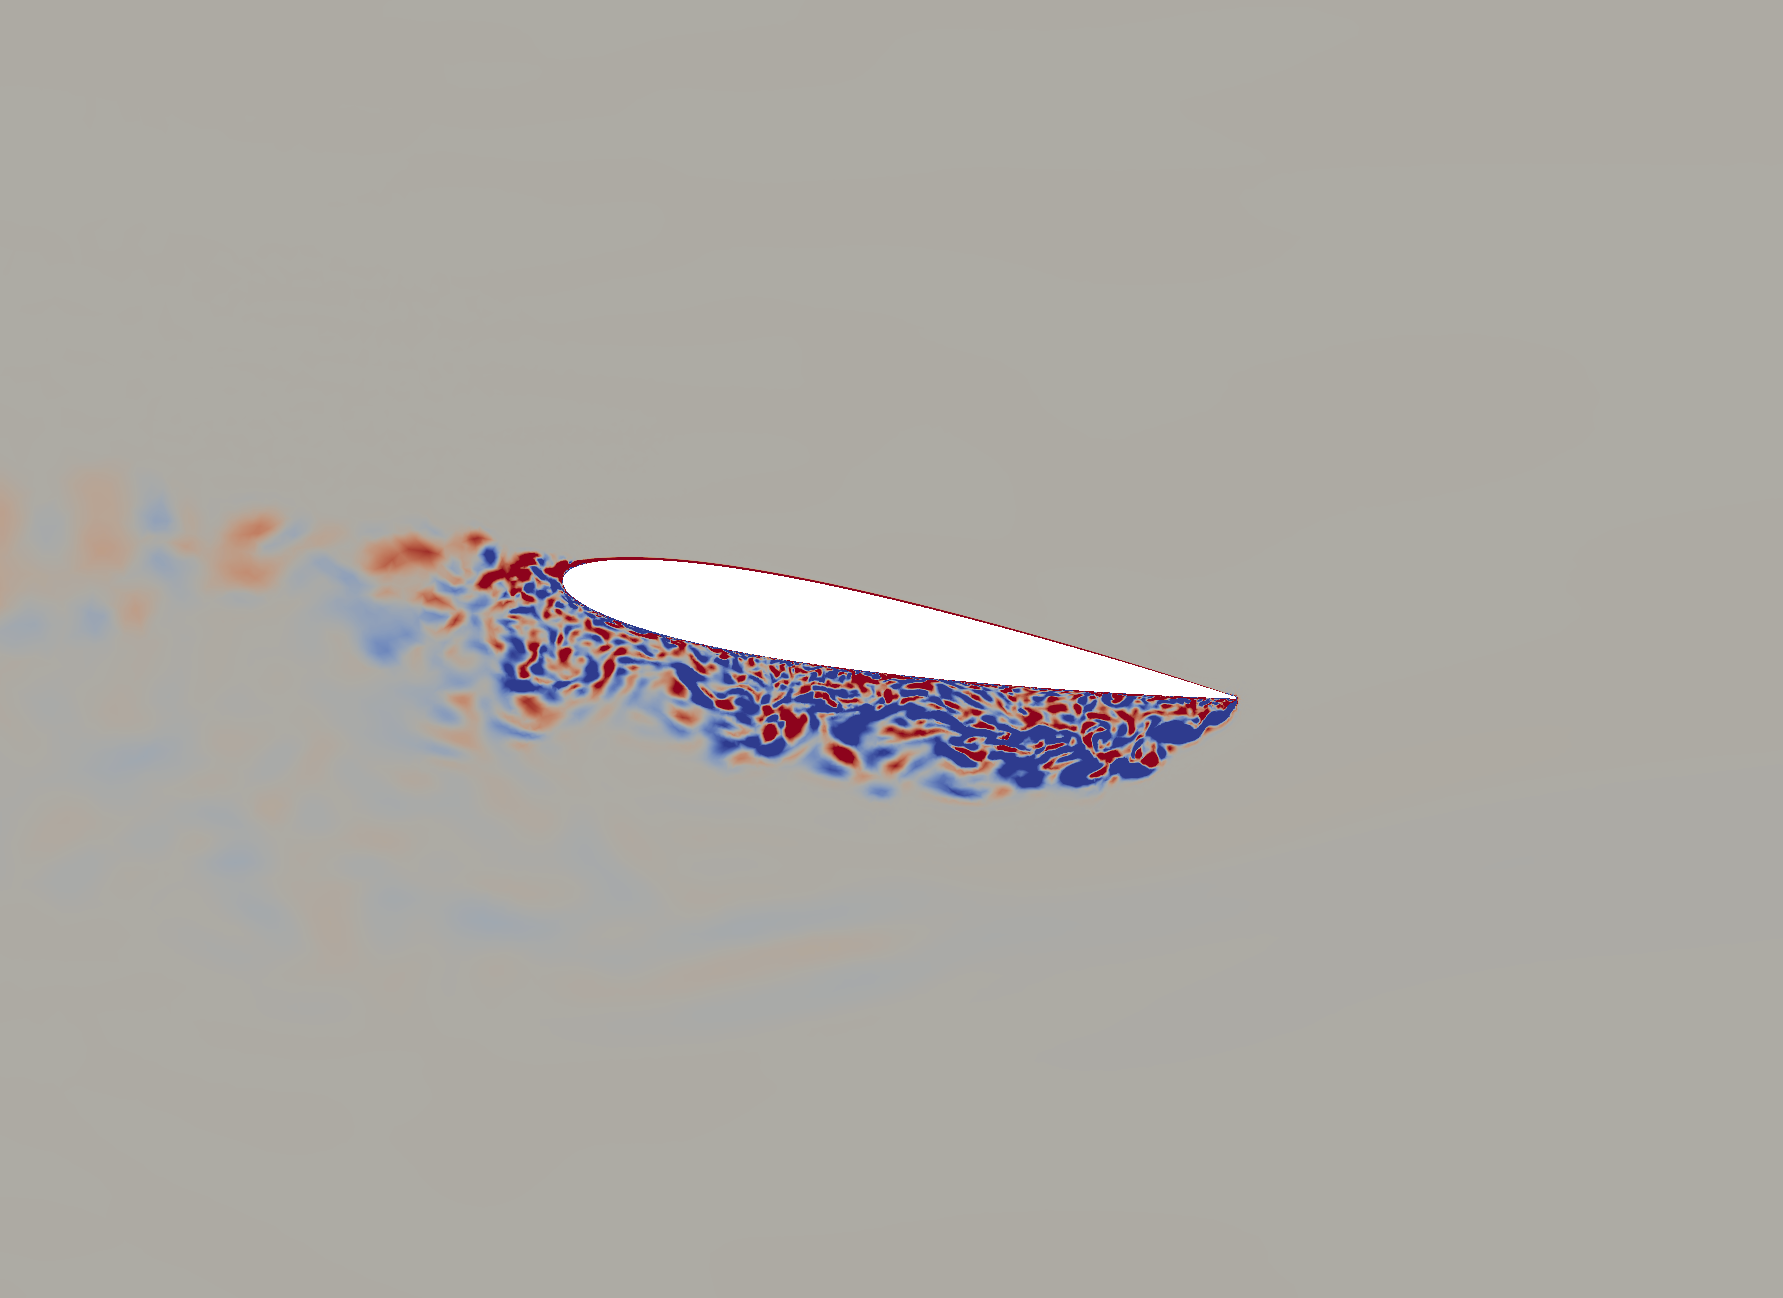
\includegraphics[width=1\textwidth]{figures/mu_2pt0/vorticity/baseline/phase_270.png}
		\caption{ $\psi$ = $270^\circ$, $\tilde{t}=0.75$}
		\label{fig:mu_2pt0_baseline_psi270}
	\end{subfigure}
	\begin{subfigure}[b]{0.4\textwidth}
		\centering
		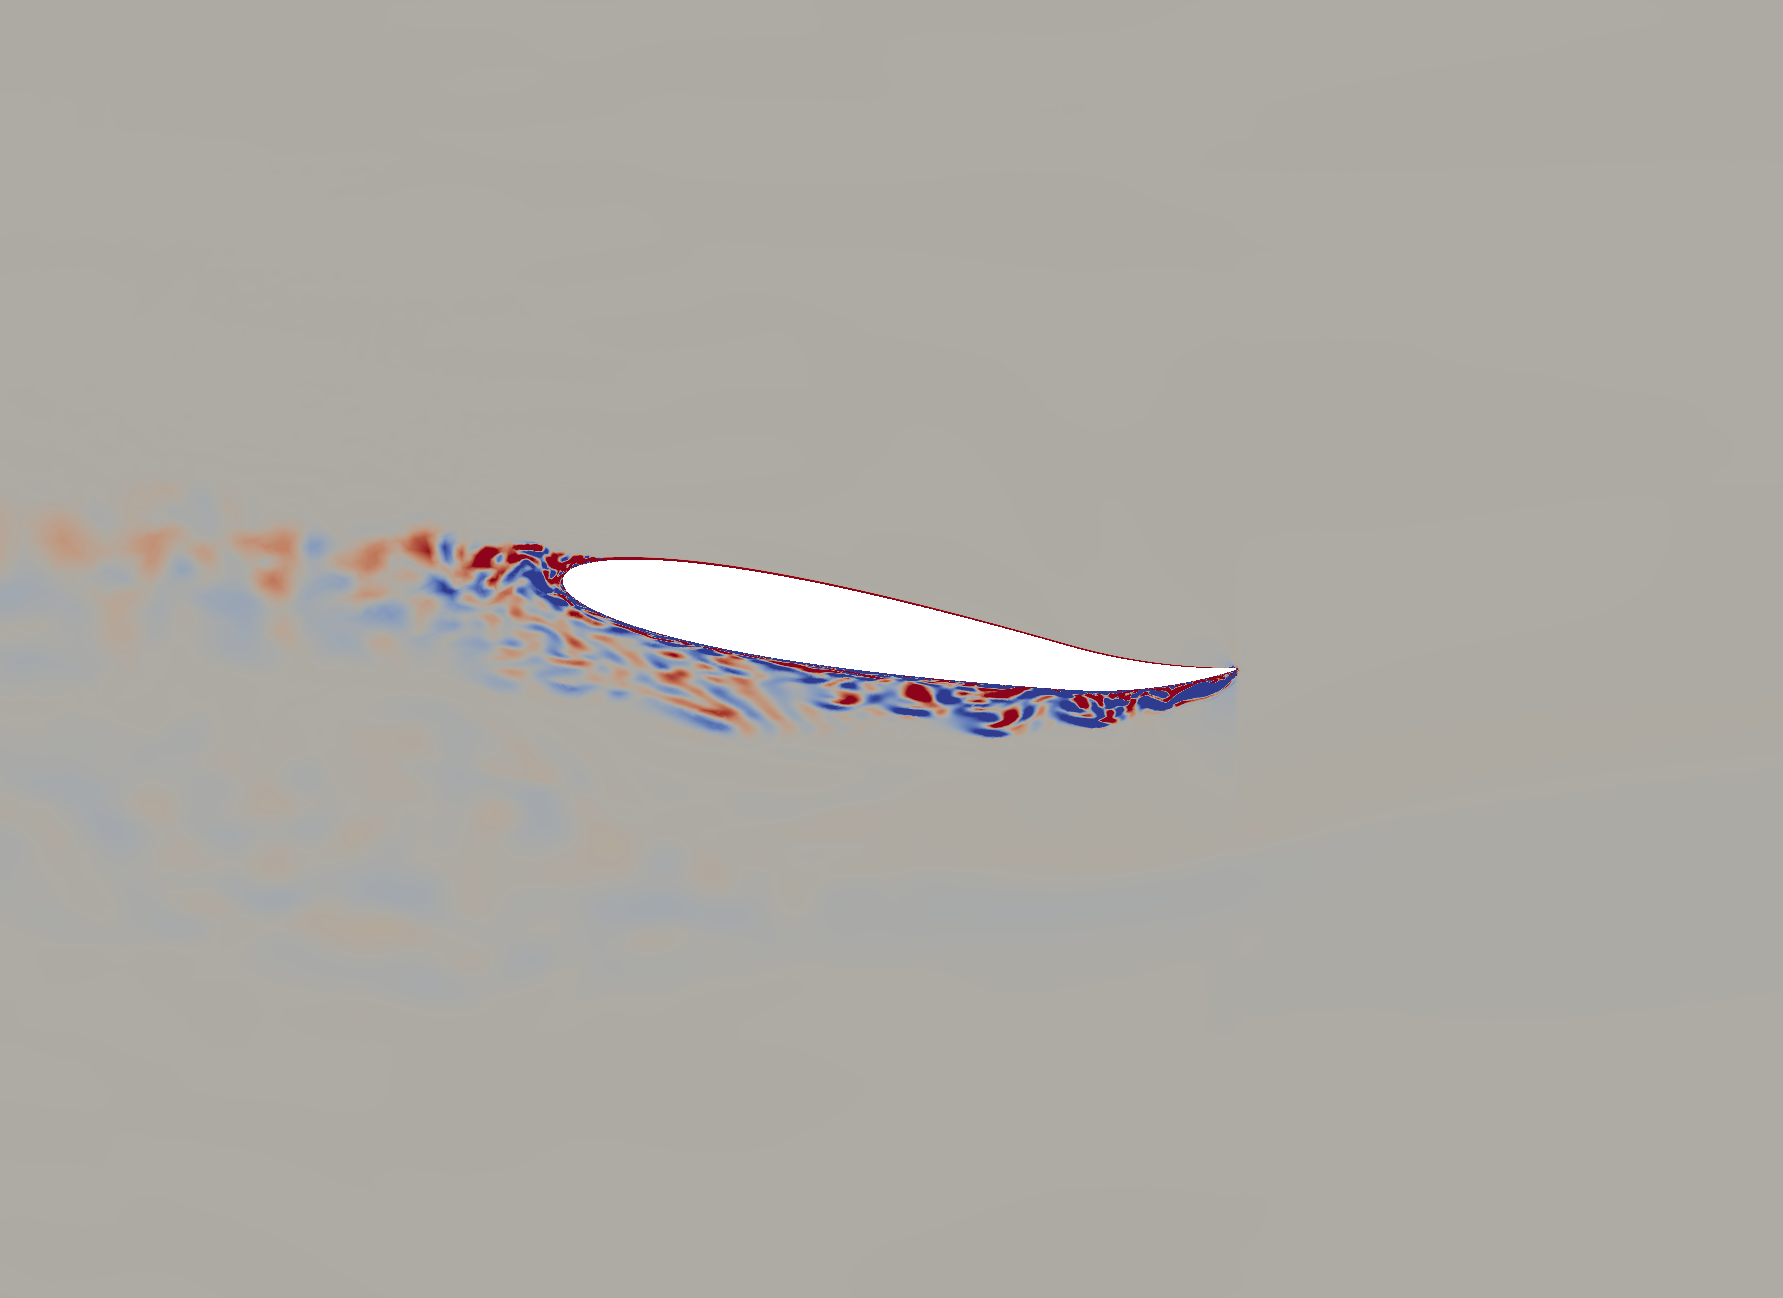
\includegraphics[width=1\textwidth]{figures/mu_2pt0/vorticity/AC/phase_270.png}
		\caption{ $\psi$ = $270^\circ$, $\tilde{t}=0.75$}
		\label{fig:mu_2pt0_AC_psi270}
	\end{subfigure}
	
	\begin{subfigure}[b]{0.4\textwidth}
		\centering
		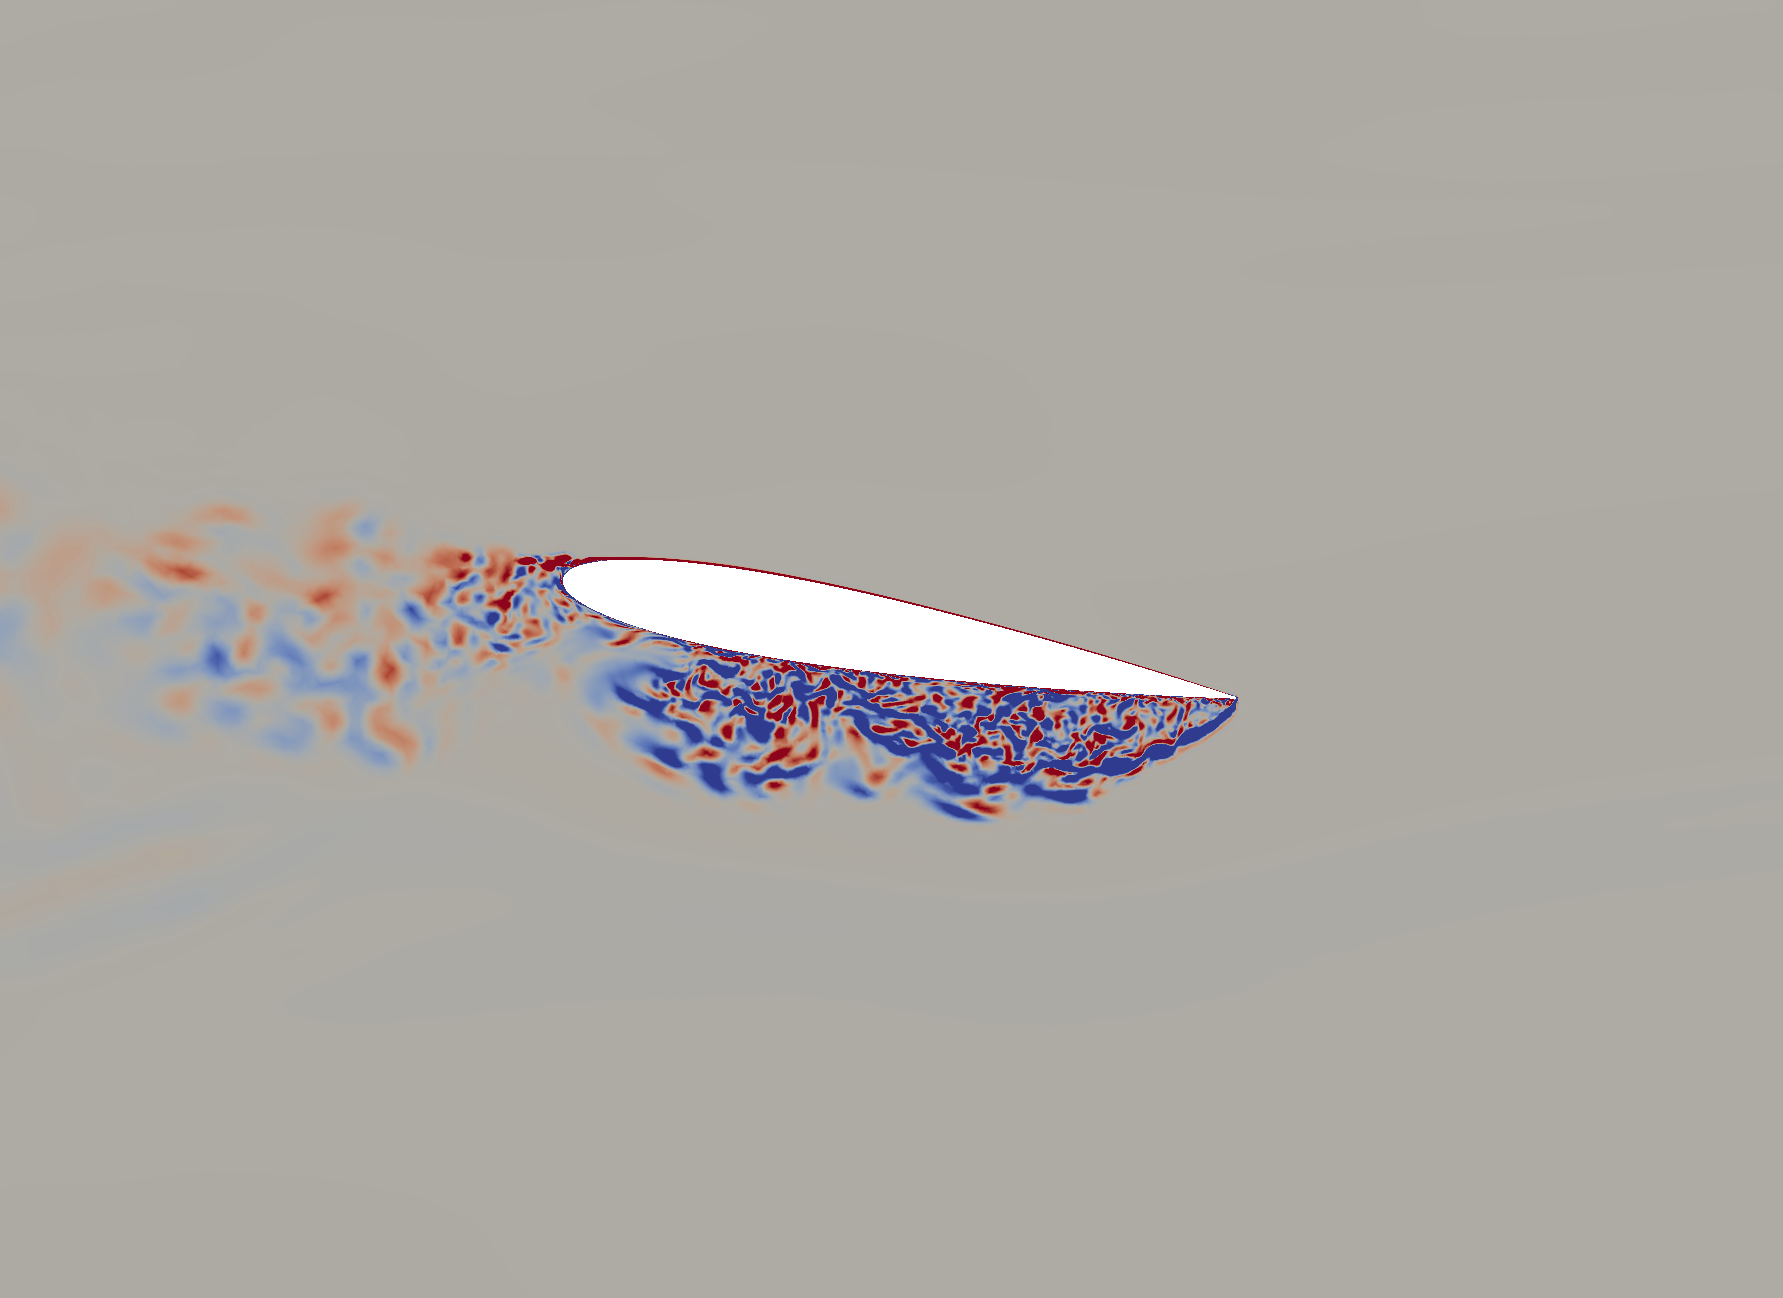
\includegraphics[width=1\textwidth]{figures/mu_2pt0/vorticity/baseline/phase_285.png}
		\caption{ $\psi$ = $285^\circ$, $\tilde{t}=0.792$}
		\label{fig:mu_2pt0_baseline_psi285}
	\end{subfigure}
	\begin{subfigure}[b]{0.4\textwidth}
		\centering
		\includegraphics[width=1\textwidth]{figures/mu_2pt0/vorticity/AC/phase_285.png}
		\caption{ $\psi$ = $285^\circ$,  $\tilde{t}=0.792$}
		\label{fig:mu_2pt0_AC_psi285}
	\end{subfigure}
	
	
	%\begin{subfigure}[b]{0.4\textwidth}
	%	\centering
	%	\includegraphics[width=1\textwidth]{figures/mu_2pt0/vorticity/baseline/phase_300.png}
	%	\caption{ $\psi$ = $300^\circ$, $\tilde{t}=0.833$}
	%	\label{fig:mu_2pt0_baseline_psi300}
	%\end{subfigure}
	%\begin{subfigure}[b]{0.4\textwidth}
	%	\centering
	%	\includegraphics[width=1\textwidth]{figures/mu_2pt0/vorticity/AC/phase_300.png}
	%	\caption{ $\psi$ = $300^\circ$, $\tilde{t}=0.833$}
	%	\label{fig:mu_2pt0_AC_psi300}
	%\end{subfigure}
	
	\begin{subfigure}[b]{0.4\textwidth}
		\centering
		\includegraphics[width=1\textwidth]{figures/mu_2pt0/vorticity/baseline/phase_315.png}
		\caption{ $\psi$ = $315^\circ$, $\tilde{t}=0.875$}
		\label{fig:mu_2pt0_baseline_psi315}
	\end{subfigure}
	\begin{subfigure}[b]{0.4\textwidth}
		\centering
		\includegraphics[width=1\textwidth]{figures/mu_2pt0/vorticity/AC/phase_315.png}
		\caption{ $\psi$ = $315^\circ$, $\tilde{t}=0.875$}
		\label{fig:mu_2pt0_AC_psi315}
	\end{subfigure}
	
	%\begin{subfigure}[b]{0.4\textwidth}
	%	\centering
	%	\includegraphics[width=1\textwidth]{figures/mu_2pt0/vorticity/baseline/phase_330.png}
	%	\caption{ $\psi$ = $330^\circ$, $\tilde{t}=0.917$}
	%	\label{fig:mu_2pt0_baseline_psi330}
	%\end{subfigure}
	%\begin{subfigure}[b]{0.4\textwidth}
	%	\centering
	%	\includegraphics[width=1\textwidth]{figures/mu_2pt0/vorticity/AC/phase_330.png}
	%	\caption{ $\psi$ = $330^\circ$, $\tilde{t}=0.917$}
	%	\label{fig:mu_2pt0_AC_psi330}
	%\end{subfigure}
	
	\begin{subfigure}[b]{0.4\textwidth}
		\centering
		\includegraphics[width=1\textwidth]{figures/mu_2pt0/vorticity/baseline/phase_345.png}
		\caption{ $\psi$ = $345^\circ$, $\tilde{t}=0.958$}
		\label{fig:mu_2pt0_baseline_psi345}
	\end{subfigure}
	\begin{subfigure}[b]{0.4\textwidth}
		\centering
		\includegraphics[width=1\textwidth]{figures/mu_2pt0/vorticity/AC/phase_345.png}
		\caption{ $\psi$ = $345^\circ$, $\tilde{t}=0.958$}
		\label{fig:mu_2pt0_AC_psi345}
	\end{subfigure}
	\caption{Instantaneous spanwise vorticity at 8 different phases for the baseline (left column) and actuated (right column) cases at $\mu_{sect}$ = 2.0}
	\label{fig:vortScreen_mu2pt0}
\end{figure}

\subsection{SC1095: $\mu_{sect}=2.0$}

\subsubsection{Force Response}

Figure \ref{fig:total_drag_zoomed_mu_2pt0_SC1095} shows the behavior of the total drag in the reverse flow region for SC1095 airfoil for the baseline and actuated cases at $\mu_{sect}=2.0$. 
Similar results to the NACA 0012 airfoil are observed here.
In the non-actuated case the drag fluctuates in the reverse flow region, while the drag is fairly monotonic in the actuated case.
In the non-actuated case, the drag exhibits a local maximum around $\psi=220^\circ$ and a local minimum around $\psi=285^\circ$.
The resulting peak-to-peak variation in the non-actuated case is substantial, as shown in Figure \ref{fig:total_drag_zoomed_mu_2pt0_SC1095}.
This peak-to-peak variation in the reverse flow region is mitigated in the actuated case.
A maximum drag reduction of up to 78\% is reported in this case.


\begin{figure}[H]
	
	\centering
	\includegraphics[width=0.75\textwidth]{figures/SC1095/Zoomed_Drag_tot_SC1095_Re1m_aoa10_2.png}
	\caption{Normalized total drag in the reverse flow region for the non-actuated (blue with open circles) and actuated (red with open triangles) cases at $\mu_{sect}=2.0$ for SC1095 airfoil}
	\label{fig:total_drag_zoomed_mu_2pt0_SC1095}
\end{figure}



\subsubsection{Flowfield: Spanwise Vorticity and Velocity Magnitude}

Figure \ref{fig:vortScreen_mu2pt0_SC1095} shows the instantaneous spanwise vorticity for the sectional advance ratio of $\mu_{sect}=2.0$.
As before, 8 different phases over the retreating phase of the cycle are shown and the vorticity range is selected to be [-30,30]$ U_{sect} /C$. Note that the set of phases shown is different between $\mu_{sect}=1.5$ and $2.0$. For this advance ratio, the airfoil enters the reverse flow region at $\psi=210^\circ$, and exits the reverse flow at $\psi=330^\circ$.
Reflex camber is activated at the phase of $\psi$=$200^\circ$ and reaches the full deflection at $\psi$=$205^\circ$.
After the airfoil exits the reverse flow, the reflexed airfoil starts returning to its undeflected position at $\psi$=$335^\circ$, and smoothly reaches its original shape at $\psi$=$340^\circ$.

Roll up of the boundary layer and LEV formation is seen for both baseline and actuated cases at $\psi$=$210^\circ$.

In the subsequent phases after $\psi$=$225^\circ$ the size of the separated region increases for the baseline case till up to $\psi$=$285^\circ$.
For the actuated case, the separated region is relatively small (see Figures \ref{fig:mu_2pt0_baseline_psi270} and \ref{fig:mu_2pt0_AC_psi270}) and its size remains fairly constant between phases $\psi$=$255^\circ$ and $285^\circ$ (see Figures \ref{fig:SC1095_AC_psi255}, \ref{fig:SC1095_AC_psi270} and \ref{fig:SC1095_AC_psi285}).
As before, overall a significant reduction is observed in the size/extent as well as unsteadiness of the separation bubble near the trailing edge during the reverse flow region due to active reflex camber.

After $\psi$=$285^\circ$, the trailing-edge flow separation begins to wash away from the airfoil for both baseline and actuated cases, see Figures \ref{fig:SC1095_baseline_psi315} and \ref{fig:SC1095_AC_psi315}. 
For the actuated case at $\psi$=$345^\circ$, the reflexed trailing edge is at its undeflected position.

\begin{figure}[H]
	\centering
	
	\begin{subfigure}[b]{0.4\textwidth}
		\centering
		\includegraphics[width=1\textwidth]{figures/SC1095/baseline/phase_195.png}
		\caption{ $\psi$ = $195^\circ$, $\tilde{t}=0.542$}
		\label{fig:SC1095_baseline_psi195}
	\end{subfigure}
	\begin{subfigure}[b]{0.4\textwidth}
		\centering
		\includegraphics[width=1\textwidth]{figures/SC1095/AC/phase_195.png}
		\caption{ $\psi$ = $195^\circ$, $\tilde{t}=0.542$}
		\label{fig:SC1095_AC_psi195}
	\end{subfigure}
	
	\begin{subfigure}[b]{0.4\textwidth}
		\centering
		\includegraphics[width=1\textwidth]{figures/SC1095/baseline/phase_210.png}
		\caption{ $\psi$ = $210^\circ$, $\tilde{t}=0.542$}
		\label{fig:SC1095_baseline_psi210}
	\end{subfigure}
	\begin{subfigure}[b]{0.4\textwidth}
		\centering
		\includegraphics[width=1\textwidth]{figures/SC1095/AC/phase_210.png}
		\caption{ $\psi$ = $210^\circ$, $\tilde{t}=0.542$}
		\label{fig:SC1095_AC_psi210}
	\end{subfigure}
	
	\begin{subfigure}[b]{0.4\textwidth}
		\centering
		\includegraphics[width=1\textwidth]{figures/SC1095/baseline/phase_225.png}
		\caption{ $\psi$ = $225^\circ$, $\tilde{t}=0.625$}
		\label{fig:SC1095_baseline_psi225}
	\end{subfigure}
	\begin{subfigure}[b]{0.4\textwidth}
		\centering
		\includegraphics[width=1\textwidth]{figures/SC1095/AC/phase_225.png}
		\caption{ $\psi$ = $225^\circ$,  $\tilde{t}=0.625$}
		\label{fig:SC1095_AC_psi225}
	\end{subfigure}
	
	
	%\begin{subfigure}[b]{0.4\textwidth}
	%	\centering
	%	 \includegraphics[width=1\textwidth]{figures/SC1095/baseline/phase_240.png}
	%	\caption{ $\psi$ = $240^\circ$, $\tilde{t}=0.667$}
	%	\label{fig:SC1095_baseline_psi240}
	%\end{subfigure}
	%\begin{subfigure}[b]{0.4\textwidth}
	%	\centering
	%	 \includegraphics[width=1\textwidth]{figures/SC1095/AC/phase_240.png}
	%	\caption{ $\psi$ = $240^\circ$, $\tilde{t}=0.667$}
	%	\label{fig:SC1095_AC_psi240}
	%\end{subfigure}	
	
	
	\caption{Instantaneous spanwise vorticity at 8 different phases for the baseline (left column) and actuated (right column) cases at $\mu_{sect}$ = 2.0 for SC1095 airfoil}
	%\label{fig:vortScreen_mu2pt0}
\end{figure}

\begin{figure}[H]\ContinuedFloat
	\centering
	
		\begin{subfigure}[b]{0.4\textwidth}
		\centering
		\includegraphics[width=1\textwidth]{figures/SC1095/baseline/phase_255.png}
		\caption{ $\psi$ = $255^\circ$, $\tilde{t}=0.708$}
		\label{fig:SC1095_baseline_psi255}
	\end{subfigure}
	\begin{subfigure}[b]{0.4\textwidth}
		\centering
		\includegraphics[width=1\textwidth]{figures/SC1095/AC/phase_255.png}
		\caption{ $\psi$ = $255^\circ$, $\tilde{t}=0.708$}
		\label{fig:SC1095_AC_psi255}
	\end{subfigure}
	\begin{subfigure}[b]{0.4\textwidth}
		\centering
		\includegraphics[width=1\textwidth]{figures/SC1095/baseline/phase_270.png}
		\caption{ $\psi$ = $270^\circ$, $\tilde{t}=0.75$}
		\label{fig:SC1095_baseline_psi270}
	\end{subfigure}
	\begin{subfigure}[b]{0.4\textwidth}
		\centering
		\includegraphics[width=1\textwidth]{figures/SC1095/AC/phase_270.png}
		\caption{ $\psi$ = $270^\circ$, $\tilde{t}=0.75$}
		\label{fig:SC1095_AC_psi270}
	\end{subfigure}
	
	\begin{subfigure}[b]{0.4\textwidth}
		\centering
		\includegraphics[width=1\textwidth]{figures/SC1095/baseline/phase_285.png}
		\caption{ $\psi$ = $285^\circ$, $\tilde{t}=0.792$}
		\label{fig:SC1095_baseline_psi285}
	\end{subfigure}
	\begin{subfigure}[b]{0.4\textwidth}
		\centering
		\includegraphics[width=1\textwidth]{figures/SC1095/AC/phase_285.png}
		\caption{ $\psi$ = $285^\circ$,  $\tilde{t}=0.792$}
		\label{fig:SC1095_AC_psi285}
	\end{subfigure}
	
		\caption{Instantaneous spanwise vorticity at 8 different phases for the baseline (left column) and actuated (right column) cases at $\mu_{sect}$ = 2.0 for SC1095 airfoil}
	%\label{fig:vortScreen_mu2pt0}
\end{figure}

\begin{figure}[H]\ContinuedFloat
\centering
	\begin{subfigure}[b]{0.4\textwidth}
		\centering
		\includegraphics[width=1\textwidth]{figures/SC1095/baseline/phase_300.png}
		\caption{ $\psi$ = $300^\circ$, $\tilde{t}=0.833$}
		\label{fig:SC1095_baseline_psi300}
	\end{subfigure}
	\begin{subfigure}[b]{0.4\textwidth}
		\centering
		\includegraphics[width=1\textwidth]{figures/SC1095/AC/phase_300.png}
		\caption{ $\psi$ = $300^\circ$, $\tilde{t}=0.833$}
		\label{fig:SC1095_AC_psi300}
	\end{subfigure}
	
	\begin{subfigure}[b]{0.4\textwidth}
		\centering
		\includegraphics[width=1\textwidth]{figures/SC1095/baseline/phase_315.png}
		\caption{ $\psi$ = $315^\circ$, $\tilde{t}=0.875$}
		\label{fig:SC1095_baseline_psi315}
	\end{subfigure}
	\begin{subfigure}[b]{0.4\textwidth}
		\centering
		\includegraphics[width=1\textwidth]{figures/SC1095/AC/phase_315.png}
		\caption{ $\psi$ = $315^\circ$, $\tilde{t}=0.875$}
		\label{fig:SC1095_AC_psi315}
	\end{subfigure}
	
	%\begin{subfigure}[b]{0.4\textwidth}
	%	\centering
	%	\includegraphics[width=1\textwidth]{figures/SC1095/baseline/phase_330.png}
	%	\caption{ $\psi$ = $330^\circ$, $\tilde{t}=0.917$}
	%	\label{fig:SC1095_baseline_psi330}
	%\end{subfigure}
	%\begin{subfigure}[b]{0.4\textwidth}
	%	\centering
	%	\includegraphics[width=1\textwidth]{figures/SC1095/AC/phase_330.png}
	%	\caption{ $\psi$ = $330^\circ$, $\tilde{t}=0.917$}
	%	\label{fig:SC1095_AC_psi330}
	%\end{subfigure}
	
	\begin{subfigure}[b]{0.4\textwidth}
		\centering
		\includegraphics[width=1\textwidth]{figures/SC1095/baseline/phase_345.png}
		\caption{ $\psi$ = $345^\circ$, $\tilde{t}=0.958$}
		\label{fig:SC1095_baseline_psi345}
	\end{subfigure}
	\begin{subfigure}[b]{0.4\textwidth}
		\centering
		\includegraphics[width=1\textwidth]{figures/SC1095/AC/phase_345.png}
		\caption{ $\psi$ = $345^\circ$, $\tilde{t}=0.958$}
		\label{fig:SC1095_AC_psi345}
	\end{subfigure}
	
	
	
	\caption{Instantaneous spanwise vorticity at 8 different phases for the baseline (left column) and actuated (right column) cases at $\mu_{sect}$ = 2.0 for SC1095 airfoil}
	\label{fig:vortScreen_mu2pt0_SC1095}
\end{figure}

